\documentclass[12pt]{scrreprt}
\usepackage[english]{babel}
\usepackage[utf8x]{inputenc}
\usepackage{lmodern,textcomp}
\usepackage[T1]{fontenc}
\usepackage{textcomp}
\usepackage{amsmath}
\usepackage{graphicx}
\usepackage{appendix}
%\usepackage[colorlinks, linkcolor=magenta, citecolor=red]{hyperref}
\usepackage[acronym, toc]{glossaries}
\usepackage{float}
\usepackage{csquotes}
\usepackage{caption}

\usepackage{listings}
\usepackage{caption}
\usepackage{minted}
\usepackage{float}
\usepackage{array}
\usepackage{tabularx}
\usepackage[table]{xcolor}
\usepackage{makecell}
\usepackage{enumitem}
\usepackage{xcolor}
\usepackage{datetime}

% https://latexcolor.com/
\definecolor{flavescent}{rgb}{0.97, 0.91, 0.56}
\definecolor{flax}{rgb}{0.93, 0.86, 0.51}
\definecolor{paleaqua}{rgb}{0.74, 0.83, 0.9}
\definecolor{paleblue}{rgb}{0.69, 0.93, 0.93}
\definecolor{periwinkle}{rgb}{0.8, 0.8, 1.0}
\definecolor{persiangreen}{rgb}{0.0, 0.65, 0.58}
\definecolor{mediumturquoise}{rgb}{0.28, 0.82, 0.8}
\definecolor{mayablue}{rgb}{0.45, 0.76, 0.98}
\definecolor{lightskyblue}{rgb}{0.53, 0.81, 0.98}
\definecolor{magicmint}{rgb}{0.67, 0.94, 0.82}

\newdate{date}{02}{06}{2020}
\date{\displaydate{date}}


\newcommand{\mq}{How can a real-time safety module be designed and implemented that prevents injury to patients or damage to the environment because of collision, clamping or pinching caused by care robot Rose?}
% Interface to Rose. Communication over ethernet, fast enough.
\newcommand{\sqone}{What hardware and operating system can be used to implement a safety module that has real-time constraints for care robot Rose?}
\newcommand{\sqtwo}{How can sensor and actuator data be retrieved?}
% Certain things that cannot be done mechanically (essentially why we need to use the safety module in the first place).
\newcommand{\sqthree}{How can sensor and actuator data be used to check for unsafe behaviour?}
% This should specify the entire deal having to do with the modelling real-time constraints in dezyne and the other means of verification of the safety module.
\newcommand{\sqfour}{How can the safety module be modelled in relation to the real-time care robot such that the model guarantees that unsafe behaviour is detected and signalled and that the safety module meets all of its deadlines?}
\newcommand{\sqfive}{How can we implement the model on the hardware and how can we implement it in software?}

 
\usepackage[style=apa]{biblatex}
%\usepackage{natbib}
\addbibresource{bib.bib}

 
\makeglossaries

% No indents after pars
\setlength\parindent{0pt}

\usepackage[colorlinks, linkcolor=black, citecolor=black]{hyperref}
%
%\DeclareCiteCommand{\cite}
%  {\usebibmacro{prenote}}
%  {\usebibmacro{citeindex}%
%   \printtext[bibhyperref]{\usebibmacro{cite}}}
%  {\multicitedelim}
%  {\usebibmacro{postnote}}
%
%\DeclareCiteCommand*{\cite}
%  {\usebibmacro{prenote}}
%  {\usebibmacro{citeindex}%
%   \printtext[bibhyperref]{\usebibmacro{citeyear}}}
%  {\multicitedelim}
%  {\usebibmacro{postnote}}
%
%\DeclareCiteCommand{\parencite}[\mkbibparens]
%  {\usebibmacro{prenote}}
%  {\usebibmacro{citeindex}%
%    \printtext[bibhyperref]{\usebibmacro{cite}}}
%  {\multicitedelim}
%  {\usebibmacro{postnote}}
%
%\DeclareCiteCommand*{\parencite}[\mkbibparens]
%  {\usebibmacro{prenote}}
%  {\usebibmacro{citeindex}%
%    \printtext[bibhyperref]{\usebibmacro{citeyear}}}
%  {\multicitedelim}
%  {\usebibmacro{postnote}}
%
%\DeclareCiteCommand{\footcite}[\mkbibfootnote]
%  {\usebibmacro{prenote}}
%  {\usebibmacro{citeindex}%
%  \printtext[bibhyperref]{ \usebibmacro{cite}}}
%  {\multicitedelim}
%  {\usebibmacro{postnote}}
%
%\DeclareCiteCommand{\footcitetext}[\mkbibfootnotetext]
%  {\usebibmacro{prenote}}
%  {\usebibmacro{citeindex}%
%   \printtext[bibhyperref]{\usebibmacro{cite}}}
%  {\multicitedelim}
%  {\usebibmacro{postnote}}
%
%\DeclareCiteCommand{\textcite}
%  {\boolfalse{cbx:parens}}
%  {\usebibmacro{citeindex}%
%   \printtext[bibhyperref]{\usebibmacro{textcite}}}
%  {\ifbool{cbx:parens}
%     {\bibcloseparen\global\boolfalse{cbx:parens}}
%     {}%
%   \multicitedelim}
%  {\usebibmacro{textcite:postnote}}



\begin{document}

% Syntax highlighting for my code.
\lstdefinestyle{customc}{
  belowcaptionskip=1\baselineskip,
  breaklines=true,
  frame=L,
  xleftmargin=\parindent,
  language=C++,
  showstringspaces=false,
  basicstyle=\footnotesize\ttfamily,
  keywordstyle=\bfseries\color{blue},
  commentstyle=\itshape\color{green!40!black},
  identifierstyle=\color{violet},
  stringstyle=\color{red},
}

\lstset{escapechar=@,style=customc}

\begin{titlepage}
    \begin{center}
        \vspace*{1cm}
            
        \LARGE
        \textbf{Design and Implementation of a Real-time Safety Module for Care Robots}
            
        \vspace{0.5cm}
        %\LARGE
        %Thesis Subtitle
            
        \vspace{1.5cm}
            
        Kaydo Alders
            
        \vfill
            
        A thesis presented for the Bachelor degree in Computer Engineering
            
        \vspace{0.8cm}
            
        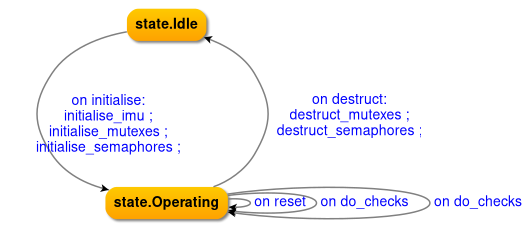
\includegraphics[width=0.8\textwidth]{Figures/results/modelling_figures/IController/IController_state_chart.png}
        
        \vspace{0.8cm}
        
        \Large
        Computer Engineering\\
        Inholland University of Applied Sciences\\
        Alkmaar, Netherlands\\
        \large \today
            
    \end{center}
\end{titlepage}

\begin{titlepage}

\newcommand{\HRule}{\rule{\linewidth}{0.5mm}} % Defines a new command for the horizontal lines, change thickness here

\center % Center everything on the page
 
%----------------------------------------------------------------------------------------
%    HEADING SECTIONS
%    HEADING SECTIONS
%----------------------------------------------------------------------------------------

\textsc{\Large Inholland University of Applied Science}\\[1.5cm] % Name of your university/college
\textsc{Bachelor Thesis Computer Engineering}\\[0.5cm] % Major heading such as course name
%\textsc{\large Minor Heading}\\[0.5cm] % Minor heading such as course title

%----------------------------------------------------------------------------------------
%    TITLE SECTION
%----------------------------------------------------------------------------------------

\HRule \\[0.4cm]
{ \LARGE \bfseries Design and Implementation of a Real-time Safety Module for Care Robots}\\[0.4cm] % Title of your document
\HRule \\[1.5cm]
 
%----------------------------------------------------------------------------------------
%    AUTHOR SECTION
%----------------------------------------------------------------------------------------

\begin{minipage}{0.4\textwidth}
\begin{flushleft} \large
\emph{Author:}\\
Kaydo Alders % Your name
\end{flushleft}
\end{minipage}
~
\begin{minipage}{0.4\textwidth}
\begin{flushright} \large
\emph{Supervisors:} \\
Cock Heemskerk \\ % Supervisor's Name
Ton Boode\\ % Supervisor's Name
Elmer Hoeksema \\ % Supervisor's Name
\end{flushright}
\end{minipage}\\[2cm]

% If you don't want a supervisor, uncomment the two lines below and remove the section above
%\Large \emph{Author:}\\
%John \textsc{Smith}\\[3cm] % Your name

%----------------------------------------------------------------------------------------
%    DATE SECTION
%----------------------------------------------------------------------------------------

{\large \today}\\[2cm] % Date, change the \today to a set date if you want to be precise
%{\large June 2, 2020}\\[2cm] % Date, change the \today to a set date if you want to be precise
%\large \displaydate{date}

%----------------------------------------------------------------------------------------
%    LOGO SECTION
%----------------------------------------------------------------------------------------

%\includegraphics{logo.png}\\[1cm] % Include a department/university logo - this will require the graphicx package
 
%----------------------------------------------------------------------------------------

\Large Research group Robotics,\\ Bergerweg 200, 1817 MN Alkmaar\\
+31 (0)72-5195774

%\begin{center}
%    
\includegraphics[width=0.5\textwidth]{Figures/inholland.jpg}
%\end{center}

\begin{figure}[H]
  \centering
  \begin{minipage}[b]{0.4\textwidth}
    
\includegraphics[width=\textwidth]{Figures/inholland.jpg}  \end{minipage}
  \hfill
  \begin{minipage}[b]{0.4\textwidth}
    
\includegraphics[width=\textwidth]{Figures/verum_logo.png}
  \end{minipage}
\end{figure}


\vfill % Fill the rest of the page with whitespace
\end{titlepage}

\pagenumbering{roman}
% Also see the format from moodle.
%%%
%Omslag
%    • niet verplicht
%    • Op de omslag staat alleen de titel, de naam van het bedrijf waar het onderzoek is uitgevoerd en de auteur (= naam van de student). De volledige gegevens staan op het titelblad.
%Titelblad
%
%
%Eerste blad na titelblad
%    • complete titel en eventueel ondertitel
%    • naam student en studentnummer
%    • datum en plaats
%    • Naam opleiding
%    • Hogeschool Inholland
%    • naam en plaats afstudeerbedrijf 
%    • naam afstudeerbegeleider
%
%    • plagiaatverklaring (zie blackboard voor een voorbeeld)
%
%Voorwoord
%(krijgt geen hoofdstuknummer)
%    • persoonlijk (gebruik de ik-vorm)
%    • bedankje
%    • niet opnemen in de inhoudsopgave
%    • kort
%
%Samenvatting
%(krijgt geen hoofdstuknummer)
%
%    • maximaal 1 pagina A4 (ongeveer 400 woorden)
%    • aanleiding en doelstelling 
%    • onderzoeksvraag en deelvragen
%    • opzet, resultaten en belangrijkste conclusies
%    • belangrijkste aanbevelingen (indien van toepassing)
%    • alleen relevante informatie
%    • kort en bondig
%    • is zelfstandig te lezen
%%%

\newpage
\mbox{}
\vfill
\section*{Plagiarism statement}
Hereby I certify that this research is own written work, except for references to prior research by others, which are properly cited. Any use of figures not made by myself I have been authorized to use by their respective authors. These are properly referenced as well.\\\\
Kaydo Alders\\
%\displaydate{date}
\today

\section*{Source code availability and documentation}
The source code for this research is available under the GPLv3 license. The source code and documentation can be found at the following URL: \href{https://github.com/Yousousen/safety-module-for-care-robot-rose}{https://github.com/Yousousen/safety-module-for-care-robot-rose}

\section*{Contact information of the author}
Name: Kaydo Alders\\
Student number: 580539\\
Email address: kaydo1@live.nl\\
Telephone: +31 6 34712780\\

\newpage
\chapter*{Abstract}

We developed a real-time safety module to provide an extra layer of safety for service robots.
We conducted a feasibility study to determine the feasibility of combining ideas from the fields of mobile robotic safety, verification of system behavior, real-time systems, and to determine the feasibility of applying the combination of these ideas to an implementation of a safety module for service robots. We found a \gls{pi} 3 with Sense HAT running Raspbian Buster with Xenomai 3 to be a feasible hardware and real-time operating system setup. Sensors on the Sense HAT are used to obtain values to use in the safety criteria. The Sense HAT's LED matrix is used to signal misses in meeting the safety criteria. Real-time operation is achieved by running threads in Xenomai's primary mode and by avoiding mode switches with the use of Xenomai's XDDP sockets.


\tableofcontents
\listoffigures
\listoftables
\newpage
\pagenumbering{arabic}

\chapter{Introduction}
\label{Introduction}
Research group Robotics at Inholland Alkmaar wants to improve the safety of care robots, as in the current state of affairs the care robots cannot guarantee safety. When a component of a care robot fails, like the grip arm, motion sensor or navigational equipment it can result in major consequences like damage to the robot's environment or injury of patients. Without guarantees that these consequences will not take place the care robots cannot be used in practice. Research group Robotics therefore wants to develop a safety module that can be attached to a care robot and will operate as fail operational system to prevent these major consequences. The safety module will constantly check if the behavior of the care robot is safe given the situation. The safety module is a safety critical real-time system, as its actions are required to be completed in a given time. The safety module provides an extra layer of safety over existing safety measures on the care robot.
%\section{Goal of the assignment}
%\label{Goal of the assignment}
% In de doelstelling beschrijf je wat je met je opdracht wilt bereiken. Hierin verwijs je naar de aanleiding.
\\\\
The goal of this research is to lay down the basis of this safety module and to design and implement a prototype of the safety module that will detect situations where the care robot performs unsafe actions, which the safety module will then signal to the environment. We will focus on an implementation for the semi-autonomous care robot \textit{Rose}, a care robot that is able to assist elderly people with every day tasks. Figure \ref{fig:assiting_the_elderly} shows a picture of robot Rose helping an elderly woman and Figure \ref{fig:rose_milking} shows robot Rose pouring milk into a cup. Robot Rose is located at Innovatielab at Inholland Alkmaar.
\\\\
The structure of the thesis is as follows. In Chapter \ref{Assignment specification} we give an in depth elaboration of the assignment. In Chapter \ref{Theoretical Background} we start by explaining various terms used throughout the research in Section \ref{Terms and defintions} and Section \ref{tROS}. We then present our conducted literature review on safety measures used in care robots, on hardware platforms of care robots and on operating systems used in care robots in Section \ref{Safety in care robots}, Section \ref{tHardware} and Section \ref{tOS} respectively. In Chapter \ref{Assignment Analysis and Research Questions} we analyze the assignment and set up our research questions from this analysis. In Chapter \ref{Research Methodology} we elaborate the methodology of the research, starting with the general methodology of the research in Section \ref{General methodology of the research}, followed by the methodologies used per subquestion in Section \ref{Methodology of subquestion 1}, Section \ref{Methodology of subquestion 2}, Section \ref{Methodology of subquestion 3} and Section \ref{Methodology of subquestion 4} respectively. In Chapter \ref{Results}, we show the results of the research, elaborated per subquestion in Section \ref{Choice of hardware and software}, Section \ref{Retrieving and Using Sensor Data}, Section \ref{Formal model of the behavior of the system} and Section \ref{Implementation}. In Chapter \ref{Conclusion} we present the conclusion of the research. Lastly, in Chapter \ref{Recommendation} we present the recommendations of the research. A summary can be found at the end of the thesis.
 
\begin{figure}[H]
    \centering
    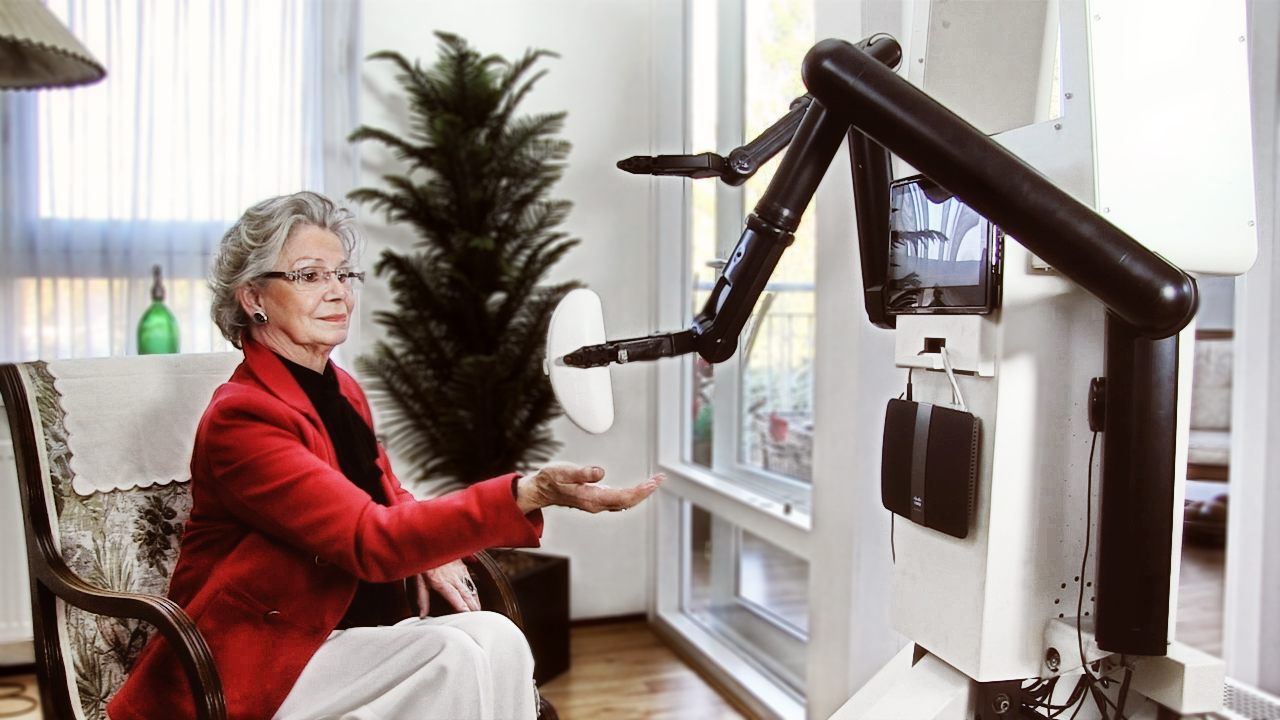
\includegraphics[width=\textwidth]{Figures/assisting_the_elderly.jpg}
    \caption{Robot Rose assisting an elderly woman, source: \cite{rose_specification}}
    \label{fig:assiting_the_elderly}
\end{figure}

\begin{figure}[H]
    \centering
    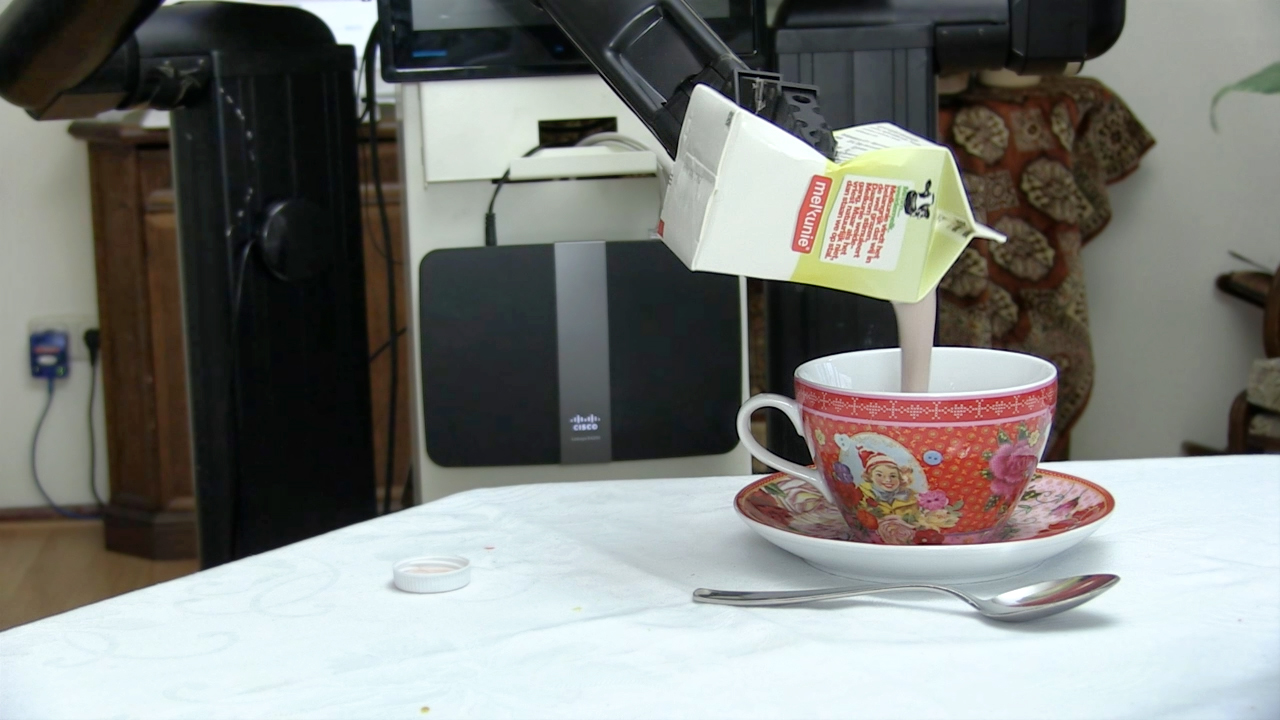
\includegraphics[width=\textwidth]{Figures/pouring_milk_into_a_cup.jpg}
    \caption{Robot Rose pouring yogurt into a cup, source: \cite{rose_specification}}
    \label{fig:rose_milking}
\end{figure}

\chapter{Assignment Specification}

\label{Assignment specification}
% In dit gedeelte beschrijf je de opdracht gedetailleerd en zo concreet mogelijk. Dit is dus een grotere uitwerking van je onderzoeksvraag.

In this chapter, an in depth elaboration of the assignment is given.
\\\\
The assignment is to design and implement a prototype of a safety module for care robots. The prototype of the safety module will focus on the semi-autonomous care robot Rose. Later models of the safety module will also have to work on different care robots, semi- and fully autonomous alike.
\par
The safety module shall detect situations where robot Rose behaves in an unsafe manner. For this assignment unsafe behavior is given the following definition:
\begin{flushleft}
\textit{Unsafe behavior is behavior that could result in injury to humans or damage to the environment by collision, clamping or pinching of the care robot with an object or human.}
\end{flushleft}
The head, body and platform can collide or clamp with an object. Pinching of an object can be caused by the grip arm's gripping force or torque. % In this section, we will further elaborate how we can design and implement a prototype of the safety module. \\
 
 %%% This is problem analysis
% From this it follows that we will look at the kinetic energy of the platform, body and head to determine its impact energy if the robot were to collide with an object. Collision as a result from Rose making a turn will be taken into account by looking at the rotational energy. Pinching can be prevented by limiting Rose her grip arm strength.
 
It should be noted that Rose already has safety measures built into her system. For example, collision with a person and electric shock due to spilling of water are prevented by using navigational path planning and by making the external housing of electrical parts water resistant (\cite{risk_analysis}). The latter is a mechanical safety measure and the former is a software safety measure, but the former is not a real-time safety measure due to the fact that Rose uses \acrfull{ros}, which is an inherently non-real-time middleware (\cite{why_is_ros_not_realtime}). In cases such as the former the goal of the safety module is to provide a second-layer real-time safety check that operates independently from Rose. The keyword real-time is important here, as this really is the added benefit over the regular safety measures. Throughout the research, we use the following definition of real-time: 

\begin{flushleft}
\textit{
A real-time system is a system that must react to stimuli from a controlled object within time intervals dictated by its environment. (\cite{realtime_systems}).
}
\end{flushleft}

Thus a real-time system is given limited time to react to given stimuli. In context of the safety module the stimulus would be, for example, the acceleration sensor on Rose detecting a large increase in velocity. In such a case the safety module would execute a real-time task to signal this large increase as unsafe behaviour to its environment. The time before which the safety module must have completed the task of signalling the environment is called the \textit{deadline} of the task. (\cite{realtime_systems}). In real-time systems a distinction is often made between hard, firm and soft real-time tasks. \cite{buttazo} gives the following definitions for these: A real-time task is said to be hard if producing the results after its deadline
may cause catastrophic consequences on the system under control, it is said to be firm if producing the results after its deadline is useless for the system, but does not cause any damage and it is said to be soft if producing the results after its deadline still has some utility for the system, even if it causes a performance degradation. These are the definitions of hard, firm and soft real-time tasks that are used throughout the research.
\\\\
From our earlier given definition of the unsafe behavior that the safety module should detect, namely that it should detect unsafe behavior that could result in injury to humans, it seems quite unethical to give the real-time safety module any other designation then hard real-time, as injury to patients is severely catastrophic. Indeed, we think the final safety module should be hard real-time. In this assignment, however, we are designing and implementing a prototype, and we will accept soft real-time behavior to be good enough for two reasons. The first reason is that the safety module will communicate with Rose to receive sensor data. As we mentioned, Rose runs \acrlong{ros}, and since \acrlong{ros} is not real-time, we cannot achieve hard real-time behavior. The problem with an inherently non-real-time system like \acrlong{ros} is that no response time can be guaranteed. This is a bottleneck, and a large part of the research is designated to accommodating for inherently non-real-time aspects of the robot-and-safety-module system like this. The second reason is that we will develop a prototype and that the development time is too little to investigate and realise the requirements for a hard real-time system. Hard real-time systems require dedicated hardware which would first have to be determined, then software would have to be developed for that dedicated hardware. A hard real-time system requires more testing as well, which cannot be achieved in the twenty weeks scope of this assignment.
\\\\
In the assignment a software model has to be made that will put some guarantees on the behavior of the safety module. For this software model, the Dezyne toolset will be used. Dezyne is a toolset that is developed by Verum, which is a partner company of this project. The reason why Dezyne is used in this research is described in Section \ref{Process algebras and Dezyne}, where the advantages of using Dezyne in this research are given and where Dezyne is compared to other options.

\section{Deliverables}
\label{Deliverables}
% Deze paragraaf bevat de specificatie van de op leveren producten zoals aangegeven door de opdrachtgever.
The deliverables of this research are as follows:

\begin{itemize}
    \item A thesis elaborating the results of the research
    \item A prototype implementation of the safety module
    \item Software models of the safety module's behavior and functionality
    \item Installation documentation of hardware and software used for the safety module
    \item Documentation of the source code, either in the respective source code files or as a separate document
\end{itemize}

\section{Involved parties}
\label{Parties involved and communication scheme}
The following table represents the parties involved in the research and their function in the research.
% Beschrijf in dit deel van je plan van aanpak welke partijen betrokken zijn bij je onderzoek. Beschrijf onder meer in welke organisatie/afdeling deze personen werkzaam zijn en wat hun functie is. Noteer hun mailadressen en telefoonnummers.
% Daarnaast vermeld je hoe de communicatie met deze personen gaat verlopen: de termijn van overleg, evt. tijdstip, de manier van communiceren et cetera.
The involved parties of this research are given in Table \ref{tab:involved-parties}. For each party, the university or company they work for, their name, their email address and their function in this research is listed.

% Please add the following required packages to your document preamble:
\begin{table}[H]
{\rowcolors{1}{magicmint}{paleblue}
\resizebox{\textwidth}{!}{%
\begin{tabular}{|l|l|l|l|}
\hline
\multicolumn{1}{|r|}{\textbf{University / Company}} & \textbf{Name} & \textbf{Contact} & \textbf{Function in research}\\ \hline
Inholland & Cock Heemskerk & cock.heemskerk@inholland.nl & Supervisor company\\ \hline
Inholland & Ton Boode & ton.boode@inholland.nl & Supervisor company\\ \hline
Inholland & Elmer Hoeksema & elmer.hoeksema@inholland.nl & Supervisor university\\ \hline
Inholland & Pieter van der Hoeven & pieter.vanderhoeven@inholland.nl & Financial insights\\ \hline
TU Twente & Jan Broenink & j.f.broenink@utwente.nl & Implementation support\\ \hline
Verum & Bert de Jonge  & bert.de.jonge@verum.com  & CEO Verum\\ \hline
Verum & Johri van Eerd & johri.van.eerd@verum.com & Modelling support\\ \hline
Heemskerk Innovative Technology & Dimitris Karageorgos & d.karageorgos@heemskerk-innovative.nl & Care robot support \\ \hline
DigiNova & Jeroen Wildenbeest & j.g.w.wildenbeest@heemskerk-innovative.nl & Acquaintance with mobile care robots \\ \hline
\end{tabular}%
}
}

\caption{Involved parties and their function in this research}
\label{tab:involved-parties}
\end{table}


\chapter{Theoretical Background and Literature Review}
In this chapter we provide the theoretical background and literature reviews that corroborate our research. We will first present definitions of terms that are used throughout this research. After that, we present our conducted literature reviews on the topics of service robot safety, hardware platforms and operating systems used in service robots. These literature reviews will serve as inspiration for the hardware and software setup for the safety module, and will help us determine proper research questions.
%Then we provide an overview of the Dezyne toolset and modelling language, the toolset and modelling language used to model the behavioral aspects of the safety module.
\label{Theoretical Background}
%\section{Practical background}
%     • waar speelt het onderzoek zich af (branche, bedrijf, afdeling)

%\section{Theoretical background}
%    • begripsafbakening (wat versta je onder de begrippen die een rol spelen bij het onderzoek? Vaak gaat het om de begrippen in de onderzoeksvraag.)
%    • eventueel eerder onderzoek 
\section{General terms and definitions}
\label{Terms and defintions}
Throughout the research we make use of a variety of terms and definitions. The definitions we use for \textit{real-time systems} and \textit{hard, firm and soft} real-time tasks were given in Section \ref{Assignment specification}. Likewise, the definition we use for \textit{unsafe behavior} was given in in Section \ref{Assignment specification} as well.% In Section \ref{Safety in care robots} we elaborate more on the safety measures used in care robots.
\\\\
Previous research frequently uses the terms \textit{mobile service robot}, \textit{domestic robot} or \textit{personal care-robot} for mobile robots used for medical (\cite{medical}) and military purposes (\cite{military}), or for use in personal care (\cite{personal}). \cite{tadele} defines a personal care-robot as a service robot with the purpose of either aiding or performing actions that contribute toward the improvement of the quality of life of an individual. \cite{tadele} defines a domestic care robot as 'a personal-care robot with or without manipulators that operate in home environments and is often mobile.' When we refer to \textit{care robots} in our research, we refer to the definition of a domestic care robot as given by \citeauthor{tadele}. We sometimes refer to service robot as well, if that is the specific term used by the research we refer to.
\\\\
In this research we refer to the concepts of \textit{processes} and \textit{threads} multiple times. A process is a sequence of execution in a computer---it is a program in execution. A process has its own address space and system resources (\cite{process_threads}). A thread is also a sequence of execution, but a thread can be seen as a subset of a process. A process can create multiple threads and each thread shares their address space and system resources with other threads (\cite{process_threads}). We sometimes use the term \textit{task} as a synonym for \textit{thread} in this research.
\par
Two other concepts related to the execution of threads are the concepts of \textit{starvation} and \textit{race-conditions}. Starvation is referred to as a situation where a thread is unable to gain regular access to shared resources and is unable to make progress (\cite{livelock_starvation}). A race condition occurs when two threads access a shared variable at the same time (\cite{race_condition}). Race conditions can be prevented by use of mutexes or semaphores. A mutex is a lockable object that is designed to signal when critical sections of code need exclusive access, preventing other threads with the same protection from executing concurrently and access the same memory locations (\cite{mutex}). Such a critical section can be a shared variable as with a race condition. A semaphore object is a synchronization object that maintains a count between zero and a specified maximum value (\cite{semaphore}). Both mutexes and semaphores can be used to prevent race conditions.
\\\\
Definitions and meanings for terms and acronyms like, \textit{\acrshort{ros}}, \textit{\acrshort{mcu}} and \textit{\acrshort{pi}} are given in our Glossary and Acronyms lists which can be accessed by clicking on the respective term or acronym.
\par
Other definitions of terms will be given as we meet them.
    

\section{Robot Operating System}
\label{tROS}
Care robot Rose uses \acrfull{ros} as its middleware. The definition of \acrfull{ros}, as given by ROS \cite{ros_wiki_introducton} is as follows:
\textit{ROS is an open-source, meta-operating system for your robot. It provides the services you would expect from an operating system, including hardware abstraction, low-level device control, implementation of commonly-used functionality, message-passing between processes, and package management. It also provides tools and libraries for obtaining, building, writing, and running code across multiple computers.}\\
 The advantages of ROS over other robotics platforms are its distributed computation model, the ability to reuse software and the rapid testing of software build with ROS. (\cite{agitr}).
 
 \section{Safety measures used for care robots}
 \label{Safety in care robots}
There are three widely used measures for safety in care robots. These are: acceleration-based criteria,  force-based criteria and energy/power-based criteria. Other criteria include human pain tolerance, maximum stress and energy density (\cite{tadele}). Of the acceleration-based criteria, the head injury criteria (HIC) is most widely used. It is a measure of the head acceleration for an impact that lasts for a certain duration (\cite{hic}). Force-based criteria consider excessive force as the possible cause of collision injury (\cite{force}). Lastly energy/power based criteria is a criteria that considers the rate of transfer of kinetic energy on body impact as the cause of possible injury to a human (\cite{crucial_milestone}).
%\par

%The prototype safety module will use a very rudimentary form of force-based and energy-based safety criteria. It will calculate the kinetic energy of the body of the care robot and force used by the grip arm of the care robot and will use this as the basis to determine what is unsafe behavior. The reason we only use this rudimentary form is because research into the topics of the various safety criteria is not the focus of this research. Instead, the focus of this research is to provide second-layer real-time safety checks on care robot Rose, meaning a safety checks that are independent of the state of Rose and her operating system. We describe the goal and specification of the assignment in more depth in Section \ref{Introduction} and Section \ref{Assignment specification} respectively.
 

\section{Hardware in service robots}
\label{tHardware}
Previous research has used a variety of hardware for their real-time mobile service robot applications. \citeauthor{delgado} used a Raspberry Pi 3 as their control architecture for its open source environment. They mention its advantages over (also open-source) embedded hardware. Developing a real-time environment on embedded hardware is complex due to its limited availability of systematic documentation and technical support. Although manufacturers often provide Linux kernel sources, often the system lacks compatibility with other software, which is an open problem in embedded development in general. \citeauthor{delgado} further note that the \gls{pi} 3 offers great compatibility with \acrfull{ros}, as \acrshort{ros} offers pre-built binaries for Ubuntu systems, and the \gls{pi} 3 is able to run Ubuntu. \acrshort{ros} supports Raspbian, the native operating system of the \gls{pi}, as well, but there are no pre-built  binaries for this operating system, which increases development time.
\par
\cite{bouchier} researched into ways to integrate \acrshort{ros} into a robot. Their research applied to a broader field of robots than just care robots, but their research is relevant nonetheless. They mention three architecture styles, namely embedding \acrshort{ros} on an integrated personal computer, the use of a proprietary embedded system with custom interface and the extension of \acrshort{ros} messaging and APIs. The embedded PC architecture style allows for full integration of \acrshort{ros} on a Linux distribution with the ability to run others \acrshort{ros} nodes besides the robot system as well. Still, default Linux is not real-time, and requires patches and frameworks to achieve soft or firm real-time performance. For the second option, the use of a custom proprietary embedded system, \cite{bouchier} describes a ROS device node can be setup to allow translation between ROS nodes and the propriety embedded interface. A recent development of the time had setup such an architecture on an Arduino (\cite{bouchier}). \cite{arduino} also use an Arduino board in their wireless sensor network control system for environmental sensing of temperature and humidity. The third architecture  option describes communication with ROS nodes by use of Remote Procedure Calls (RPC). Rosserial is an approach that can be used to relay messages between ROS nodes to an embeddded system. Rosserial offers support for any platform that supports the C++ programming language.
\par
The architecture styles that \citeauthor{bouchier} describes are focused on the control system of a robot itself. In our case, the safety module is an addition to the already existing care robot system. The system of robot Rose most closely resembled the first architecture \citeauthor{bouchier} describes, but without real-time patches or a real-time framework installed. %\citeauthor{bouchier}'s research is relevant nonetheless to see what kind of architecture options exist.
\par
Another architecture not described by \citeauthor{bouchier} but which can be found in, for example, \cite{spencer} is the use of a base CPU in the robot itself, which communicates with another PC to receive input to determine which actions to take. \citeauthor{spencer} used this in a service robot that guides and informs passengers in airports. Robot Rose has a similar architecture in that she receives navigational commands from the operator connected to her via a laptop on the WiFi network. 
\par
Instead of a PC one could also use a Field Programmable Gate Array (FPGA) as main processing unit in a service robot, as \citeauthor{visual_xenomai} have done in their patrol service robot, in which the FPGA is used for image processing to calculate a travel route for the patrol robot. 
\par
Lastly, microcontrollers are also used in robotic control applications (\cite{microcontroller1}) (\cite{microcontroller2}).
%An advantage of using a microcontroller for the safety module would be that it does not add yet another PC with operating system to the system (Rose already has \texttt{rosepc1} and \texttt{rosepc2} which are PCs running Linux distributions) and a microcontroller is lower on power.

\section{Operating systems on service robots}
\label{tOS}

Service robots often run Linux distributions. As \citeauthor{delgado} describe, this is due to the fact that Linux operating system are the most popular open-source operating systems, and due to the development of real-time extensions for the Linux kernel to increase its response time and make it more suitable for real-time applications. Another reason Linux operating systems are popular is because \acrshort{ros} runs on Linux. In Section \ref{tHardware} we have seen that \cite{spencer} and \cite{delgado} use \acrshort{ros} as middleware on their service robots, and others do too, for example \cite{dimitris} in their Human aware autonomously navigating care robot, \cite{rosuser1} in their architecture design for care robots used for elderly care, \cite{intelligent_rosuser} in their service robot for customer services in hotels, \cite{rosbot_rosuser3} in their social robot used in research and education, and many more. Since all these studies use ROS as their middleware, they use Linux distributions as their operating system. The most used Linux distribution for ROS systems is Ubuntu, as it is best supported Linux distribution (\cite{foundation}), but ROS can be compiled for Raspbian as well (\cite{delgado}).
\\\\
On Linux distributions, there are two prominent options to add real-time support to the operating system. The first is Real-time Linux (\cite{rtwiki}), which applies a set of patches to the Linux kernel to make normally blocking sections of the Linux kernel preemptive. Blocking sections in the kernel refer to sections that are waiting for some event to happen before they continue executing. A preemptive kernel is one that can be interrupted while executing its code (\cite{blocking}). This is advantageous for real-time systems in that no running code will block the entire operating system waiting for some resource or event. The Real-time Linux approach is a single kernel approach, opposed to the second prominent option: the co-kernel approach of Xenomai 3 (\cite{xenomai}). In the co-kernel approach of Xenomai, a second kernel, by the name of \textit{Cobalt}, runs alongside the standard Linux kernel. The cobalt kernel schedules real-time threads and handles all time-critical activities. Real-time operation is achieved because the Cobalt kernel's activities have a higher priority than that of the standard Linux kernel (\cite{xenomai}).
\par
Xenomai imitates various other real-time operating systems by providing interfaces of them using APIs, called Xenomai \textit{skin}s. Among the Xenomai skins there is the POSIX skin, which provides POSIX functionality wrapped in real-time Xenomai functionality, and the native skin, which is Xenomai's own interface to real-time functionality. All Xenomai skins share a common core (\cite{faq}), making the skins as the name suggests, just an interface to the real-time functionality Xenomai provides.
\\\\
% Describe comparison
\cite{brown_martin} compare the Real-time Linux and Xenomai approaches and provided a number of important results. They found that for hard real-time performance Xenomai performed better than the real-time patched Linux kernel. They further made the distinction between 95\% hard real-time performance and 100\% hard real-time performance, where 95\% hard real-time means the real-time requirements should be met 95\% of the time, and where 100\% hard real-time means the real-time requirements should be met 100\% of the time\footnote{It is interesting that the paper by \citeauthor{brown_martin} makes the distinction between 95\% and 100\% hard real-time, while the notions of soft and hard real-time themselves already exist to avoid ambiguity between 'X\%' and 'Y\%' real-time. We think they make the distinction between 95\% and 100\% in order to avoid having to deal with the even more hard real-time notion they defined: life-safety hard real-time, which they explicitly stated to not focus on in the paper.}. They also made the distinction between code running in userspace and code running in kernelspace. userspace code is code that runs outside of the kernel and that the kernel is not aware of. On the contrary, kernelspace code is code that is run and maintained by the kernel (\cite{blocking}). Their tests show that for 95\% hard real-time requirements Xenomai userspace performed better than real-time patched Linux kernel userspace. For 100\% real-time requirements Xenomai kernelspace performed the best. So if one wants to have the best real-time performance one should go for Xenomai kernelspace. The downside of Xenomai kernelspace is that it is very maintenance intensive due to the use of custom built kernels, compared to Xenomai userspace (\cite{brown_martin}).

\section{Modelling and Dezyne}
\label{Modelling and Dezyne}
% TODO: Gloss dezyne
% TODO: Gloss mCRL2
Dezyne is a software modelling toolset developed by Verum (\cite{verum}), a partner company of this research. Dezyne allows us to verify the behavior of the safety module, by tracing every possible execution sequence and stopping at a problem. Dezyne's verification checks the system on the occurrences of race conditions, deadlocks, livelocks, mismatches between specification and implementation and asserts that the behvior of a program is deterministic. Dezyne has the ability to generate source code from the model specification, which makes sure that the source code is free from the aforementioned execution problems (\cite{dzntut}).
To provide this verification Dezyne internally makes use of the process algebraic language \textit{mCRL2}, a formalism for behavioral specification and verification of concurrent and distributed systems (\cite{mcrl2}). mCRL2 extends the algebra of communicating processes with various features including notions of data, time, and multi-actions.
\par
An introduction to the features of Dezyne alongside an example is given in Appendix \ref{Short introduction to the Dezyne toolset}.

\subsection{Process algebras and Dezyne}
\label{Process algebras and Dezyne}
In this subsection, we will compare Dezyne to process algebraic languages. Let us use as examples the languages mCRL2, which was mentioned in the introduction of Section \ref{Modelling and Dezyne}, and \textit{FSP}, an open-source language and model checking toolset (\cite{ltsa}). Both mCRL2 and FSP are formal specification languages that can be used to model system behavior. System behavior is the series of actions a system can perform in a particular state. Both mCRL2 and FSP allow you to verify this modelled behavior. Dezyne does not differ from the functionality of these toolsets in the sense that it allows you to model and verify behavior as well. However, where it does differ is in language and syntax. Process algebras like mCRL2 and FSP have very specific language and syntax that requires one to be versed in math. Dezyne differs from these languages in that the Dezyne modelling language's syntax resembles the syntax of the C programming language-families. This allows developers who are not experts in modelling system behavior to create deterministic deadlock- and livelock free programs. We will look at the syntax of the Dezyne modelling language in Section \ref{The Dezyne toolset and the Dezyne modelling language}.
\par
Another important matter where Dezyne differs from the process algebras mCRL2 and FSP is that Dezyne allows one to generate source code from the verified model. This source code can then be integrated into the system. In contrast to having a well verified model and hoping that one does not introduce any bugs in the process of converting this model into executable code, Dezyne's generated source code checks whether one has implemented all aspects of the model correctly. Furthermore, unlike process algebras like mCRL2 and FSP, Dezyne provides suggestions as to how to solve verification errors. This feature helps programmers to find and solve errors in a more convenient manner. This feature is shown in Section \ref{Generating code from a verified Dezyne model} of Appendix \ref{Short introduction to the Dezyne toolset}.



\chapter{Assignment Analysis and Research Questions}
\label{Assignment Analysis and Research Questions}
In this chapter, we provide an analysis of the assignment in terms of hardware choice, operating system choice and system design. In the first four sections this analysis is elaborated. In the last section, we will set up research questions based on this analysis and the Theoretical Background and Literature Reviews of Chapter \ref{Theoretical Background}.
%\section{Relevance of the assignment}
%\label{Relevance of the assignment}
% Beschrijf in de aanleiding waarom het bedrijf wil dat je deze opdracht gaat doen. Wat zijn bijvoorbeeld de consequenties voor het bedrijf wanneer de opdracht uitgevoerd wordt, of juist niet uitgevoerd wordt? Zo schets je de achtergrond en het belang van je opdracht voor het bedrijf.



\section{Hardware setup}
\label{Hardware setup}
%In this subquestion we will look at the hardware setup and see if the safety module can be implemented in such a way that the safety module could be attached to different care robots with little configuration. Further discussion on this can be found in Section \ref{}.

In Section \ref{tHardware}, we have seen the various hardware setups that previous research used on their service robots. There we saw the hardware used on the service robot itself, while the safety module will be an independent component to be attached to the care robot. We therefore have to research which hardware setup works well for our specific case.
\par
Additionally, the following are requirements for the safety module as they were conducted for the assignment:

\begin{enumerate}
    \item The hardware supports environments with real-time constraints. \label{hsOne}
    \item The hardware is able to communicate with care robot systems that run \acrlong{ros} to receive sensor data from such care robots. \label{hsTwo}
    \item The hardware has or supports the addition of a WiFi module for communication with the operator that controls the care robot. \label{hsThree}
    \item The hardware has or supports the addition of a 4G network module. \label{hsFour}
    \item The hardware has or supports the addition of an accelerometer, a gyroscope and a camera. \label{hsFive}
    \item The hardware can be attached to a care robot without impact on the operation of the care robot. \label{hsSix}
    \item The costs for the safety module do not exceed €300,- \label{hsSeven}
\end{enumerate}

Item \ref{hsOne} specifies that the hardware should support an environment with real-time constraints. In Chapter \ref{Assignment specification} we elaborated why this is required for the safety module.
\par
Item \ref{hsTwo} specifies that the hardware is required to communicate with care robot systems that run \acrfull{ros} to receive sensor data from. Robot Rose runs ROS, and many other care robots and mobile servant robots do too ((\cite{human-robot}), (\cite{spencer}), (\cite{delgado}), (\cite{dimitris}) to name a few), so if the safety module is extended to work with other care robots in the future it is very useful to support interaction with \acrshort{ros}. 
\par
Item \ref{hsThree} specifies that the hardware should support a connection over WiFi to communicate with the operator of Rose. This is because Rose is a semi-autonomous care robot robot and receives navigation input from her operator over a WiFi network connection. In Item \ref{hsFour} the requirement of a 4G network module is listed. This 4G module serves as backup module for when the WiFi connection is very weak or completely gone. Research into an appropriate 4G module is out of the scope of this assignment and will such research will be conducted for a later version of the safety module instead. Nonetheless, the hardware platform should support the addition of such a 4G module, which is why its support is listed as a requirement.
\par
Item \ref{hsFive} lists the requirement that the safety module should support the addition of sensors which it can utilize independently from the care robot to sense the environment. This should be at least an accelerometer to measure acceleration , a gyroscope to measure angular velocity, and a camera that allows the safety module to observe the environment. These independent sensors are required for two reasons. The first reason is so that the safety module does not depend on the correct operation of the sensors of the care robot. Various sensors on the safety module could break, and the safety module is supposed to do at least a subset of sensing the environment independently. The second reason is that there may be a lot of latency in receiving sensor data as it received from \acrshort{ros}. The camera will not be utilized in this assignment, but the addition of a camera should be supported for future versions of the safety module. 
Item \ref{hsSix} refers to the fact that the safety module should be portable, that is, it should be easy to attach to a care robot and it should not have an impact on the performance of the care robot. This means it should be light (relative to the care robot) and should not have large components sticking out.
\par
Lastly, Item \ref{hsSeven} specifies the maximum costs of the safety module.


\section{Operating system of the safety module}
In Section \ref{tOS}, we saw the operating systems that previous research have used on their service robots.
As a hardware setup to handle the real-time constraints of the safety module is required, likewise a software setup that can handle the real-time constraints is required. Besides that, we also have to take into account that the safety module needs to communicate with \acrshort{ros}. In Section \ref{tOS} we saw two prominent options of real-time operating system frameworks, namely that of Real-Time Linux and Xenomai. Research will be conducted to decide which option works best for the safety module.


\section{Retrieving sensor data from Rose}
\label{Retrieving sensor data from Rose}

The information about the environment obtained through sensors on the safety module can be used to measure the safety of actions of the care robot. In Section \ref{Safety in care robots} we have seen that the three most widely used safety criteria are acceleration-based criteria, force-based criteria and energy based criteria. Decisions will have to be made on what kind of safety criteria to use on the safety module. Furthermore, the safety module has the option to independently sense the environment by use of on board sensors and the option to communicate with the care robot to obtain sensor data through ROS. In Section \ref{tHardware} we have seen multiple ways to obtain data through ROS.

%Rose runs a Linux distribution with Robot Operating System (ROS) as middleware. To retrieve data from Rose her sensors we have to look into the available means of communication with this system. ROS is not real-time (\cite{why_is_ros_not_realtime}), therefore it is important to research the impact this has on the safety module and whether communication over the available interfaces is fast enough for a system with real-time constraints. %It could be that the available interface is too slow for real-time communication. Such a case is a risk and will be elaborated in Section \ref{Risks and solutions}. The obtained sensor data will be compared with a set of \textit{limit} values in a control loop.

\section{Modelling the safety module}
\label{Modelling the safety module}
% Describe things concerning research into toolset to use (Dezyne) to validate deadlines are met.
% Describe further the modelling because we do not want to model the entire robot but only what is relevant for us.

In a software model the safety module and its relation to the care robot should be modelled. A well made software model helps in determining the complexity of a problem, and it helps in breaking up the complexity of the problem into smaller parts. It is preferable to do as much verification on the state of the safety module and its actions as is possible. Such verification encompasses going through all the states of the sytem and verifying no deadlocks and livelocks occur.
A deadlock is an event that occurs in a system when all its constituent processes are blocked. Another way of saying this is that a system is deadlocked because there are no eligible actions that it can perform (\cite{ltsa}). One example of a deadlock in a system is a system in which two threads each hold a resource that the others requires to continue execution. A livelock is an event that occurs in a system where a thread's further execution requires the action of another executing thread, but the other thread is constantly served more work to do without executing the required action, meaning the first thread cannot continue to execute (\cite{livelock_starvation}).
\par
%The interactions of the safety module with the care robot need to be modelled in such a way that the real-time constraints of the system can be tested and validated. 
%In Section \ref{Modelling and Dezyne} we have introduced the Dezyne toolset developed by partner company Verum which we will use in 

\section{Principal research question and research subquestions}
\label{Principal research question and research subquestions}
% De onderzoeksvraag is het hart van het onderzoek. In één zin geef je aan wat je opdracht inhoudt. 
% In de regel verdeel je de onderzoeksvraag vervolgens in drie tot vijf deelvragen.
Having made our problem analysis we can setup our principal research question and research subquestions. To fulfill the goal of the assignment described in Chapter \ref{Introduction} and Chapter \ref{Assignment specification}, the following question will be central to the research and will serve as the principal research question:

\begin{flushleft}
\textit{\mq}
\end{flushleft}

To answer the principal research question, four subquestions are set up. The first subquestion deals with the hardware and operating system that can be used for the implementation of the safety module. Because the safety module is a safety critical real-time system, we need hardware and an operating system that can handle the real-time constraints of the care robot. The goal of the first subquestion is to provide an answer to this matter:

\begin{flushleft}
1. \textit{\sqone}
\end{flushleft}

%As This mainly concerns the capabilities of the operating system and whether the scheduler of the operating system can schedule tasks in such a way that deadlines will not be missed. Subquestion five is as follows:
%
%\begin{flushleft}
%2. \textit{\sqfive}
%\end{flushleft}

Having determined our hardware setup and operating system, we can look at ways to communicate with care robot Rose and the sensors available on our hardware. Concretely, we will look at how sensor and actuator data can be retrieved and how it can be used to detect unsafe situations. Therefore, the second subquestion is as follows:

\begin{flushleft}
2. \textit{\sqtwo}
\end{flushleft}

After subquestion two we can start designing the safety module with a software model. In the software model we want to do as much verification on the state of the safety module and its actions as possible. Moreover, we have to take into account that the safety module will be a safety critical real-time system, as described in Section \ref{Assignment specification}.
We therefore have to concern ourselves with the real-time constraints while modelling the safety module. The third subquestion, is, therefore, as follows:

\begin{flushleft}
3. \textit{\sqthree}
\end{flushleft}

The fourth and final subquestion will bring everything together into an implementation of the safety module. Here we will implement the safety module on the chosen hardware and operating system and implement the safety module according to the model of the previous subquestion. The last subquestion is, therefore, as follows:

\begin{flushleft}
4. \textit{\sqfour}
\end{flushleft}

%%%%%%%%%%%%%%%%%%%%%%%% Research Methodology %%%%%%%%%%%%%%%%%%%%%%%%
\chapter{Research Methodology}
\label{Research Methodology}
%    • per deelvraag uitwerken
%    • welke methoden zijn er gebruikt om informatie te verzamelen? Hoe ziet deze eruit? Waarom gekozen voor deze methode? Geef een toelichting. 
%    • bij interviewen: welke mensen (functies) heb je geselecteerd? Waarom?
%    • geef aan hoe je ervoor hebt gezorgd dat de informatie betrouwbaar  en valide is.
%    • geef aan hoe je de informatie hebt geanalyseerd.
%\chapter{Practical and Theoretical Background}
In this chapter, we elaborate the methodology of the research, starting with the general methodology of the research in Section \ref{General methodology of the research} followed by the methodologies used per subquestion in Section \ref{Methodology of subquestion 1}, Section \ref{Methodology of subquestion 2}, Section \ref{Methodology of subquestion 3} and Section \ref{Methodology of subquestion 4} respectively.


\section{General methodology of the research}
\label{General methodology of the research}
The general methodology of this research is a feasibility study in the sense that we want to explore existing research in robotic safety, real-time systems that deal with inherently non-real-time elements and verification of system behavior. The goal is to apply these existing ideas to our case with care robot Rose, namely to implement a prototype safety module to show the feasibility of applying the combination of these ideas to the case with care robot Rose. Because of this broad focus we only touch the surface of the vast sea of knowledge that is contained in each of these subjects. To elaborate, in the context of real-time systems we will not aim for hard real-time performance of the safety module, despite care robot Rose being perceived as a hard real-time system, as this requires much more specialised attention to implement, which would deviate from our aim to explore a multitude of ideas. Instead, we aim for the safety module to be a soft real-time system that is able to show the feasibility of the system as a whole. In the context of robot safety, we will look at the safety criteria and safety measures in existing research, but we will only apply a rudimentary form of these safety measures and safety criteria. Likewise, we explore the ideas of system behavior verification in so far this gives guarantees on the correct operation of the safety module.
\\\\
The results of this research and the prototype safety module developed in this research can be used to build further upon the ideas explored. Specifically, this research can be used to continue the development of the safety module into a product that provides an extra layer of safety to different care robots and perhaps different mobile service robots in general.% Chapter \ref{Recommendation} elaborates follow-up research options in more depth. 
\\\\
To provide answers to the subquestions stated in Section \ref{Principal research question and research subquestions}, a mixture of research methods are used. These are elaborated in the following sections.

%\section{Methodologies per subquestion}
%\label{Methodologies per subquestion}

\section{Methodology of subquestion 1}
\label{Methodology of subquestion 1}
The first subquestion stated in Section \ref{Principal research question and research subquestions} is: '\sqone'. For this subquestion, a literature review is conducted to determine what kind of hardware and operating system former studies have used in their robotic applications, and to determine whether these hardware and software setups can be used for the safety module. To do this, a variety of research papers are studied. The criterion is that the robots being developed in the research are service robots. Service robots are a superset of care robots, and are thus relevant to our research. It is an advantage if the service robot is applied to a realtime environment. Furthermore, preference is given to peer reviewed work, but the work need not necessarily be peer reviewed. A comparative study is made to analyse and interpret the information found in the literature review. A choice for the hardware and the software will then be made based on the findings of this literature review and the requirements of the safety module. The results of the comparative studies on the hardware and on the software can be found in Section \ref{Main component} and Section \ref{Operating System} of the Results chapter respectively.

% comparative study will be conducted to determine what is the best choice for the heart of the system, the processing unit, RAM and related peripherals. From here on we will determine what measuring devices can be used with this hardware, and we will conduct another literature review and comparative study to find an appropriate real-time operating system for this hardware of the safety module. The literature review on the hardware and software can be found in Section \ref{tHardware} and Section \ref{tOS} respectively. 

\section{Methodology of subquestion 2}
\label{Methodology of subquestion 2}
Similar to the first subquestion, for the second subquestion, '\sqtwo', a literature review is conducted. The literature review for the second subquestion serves to investigate the solutions of former studies in the recognition of unsafe behavior of a service robot in a given environment. The criterion for these solutions is that they are at least possible to implement with an accelerometer, a gyroscope and a camera, as these are the required hardware sensors listed in the requirements of the safety module in Section \ref{Hardware setup}. Following the literature review, we build further upon the the results of the comparative studies of the first subquestion to find out how, with the chosen hardware and software, we can interact with sensors to retrieve data, and how we can use that data to detect unsafe behavior. The results of this subquestion are elaborated in Section \ref{Retrieving and Using Sensor Data} of the Results.

\section{Methodology of subquestion 3}
\label{Methodology of subquestion 3}
The third subquestion, '\sqthree', aims to answer the question of how to model the behavioral aspects of the safety module. The result of this subquestion will be a formal specification that can put some guarantees on the behavior of the safety module. Specifically, the model will put guarantees on deadlock and livelock free operation, and the model will guarantee expected behavior to take place given enough resources. The modelling language used to to write this formal specification is Dezyne. The reasons for using Dezyne over other modelling toolsets were elaborated in Section \ref{Process algebras and Dezyne}.
\par
The correct operation of the safety module will first be validated using behavior verification checks, which are checks in the model itself. After that the correct operation of the safety module will be validated using software latency and statistics tests. The second is a topic for subquestion 4. For the first we will make use of Dezyne's behavior verification system. Examples of this verifier can be found in Section \ref{Verifying a Dezyne model} of Appendix \ref{Short introduction to the Dezyne toolset}.
\par
Dezyne allows us to generate source code from the formal specification model, which assures that the deadlock and livelock free operation of the safety module as is validated in the model is carried over to the implementation. We will use this feature to generate C++ code. This C++ code will be integrated with the rest of the implementation code. An example of the generation of source code can be found in Section \ref{Generating code from a verified Dezyne model} of Appendix \ref{Short introduction to the Dezyne toolset}.
\par
The results of this subquestion are elaborated in Section \ref{Formal model of the behavior of the system} of the Results.

\section{Methodology of subquestion 4}
\label{Methodology of subquestion 4}
The fourth and last subquestion, '\sqfour' will put everything together in an implementation of the formal specification on hardware and software. In the process of answering this subquestion we will conduct two kinds of tests to test the operation of the safety module. The first test that will be performed is a latency test, using the Linux program \texttt{latency}. With this test we want to test the time it takes for the system to respond to given stimuli. Two latency tests will be performed---one with and one without the safety module program running. The latency test program will run for 20 seconds, trying to schedule test tasks and measure the response times. The test will compute the minimal, average and maximal latency.
\par
The second test that will be performed is a CPU load and process statistics test, using the Linux program \texttt{stat}. Both \texttt{latency} and \texttt{stat} are programs that come with the operating system and are thus well supported by it. Besides gaining insights on the general resource usage of various parts of the safety module system, what we are mainly interested in with this test is testing whether the processes, or tasks of the system, are capable of supporting a real-time environment. Thus, the result of this test provides an answer the queston of whether the safety module can be considered a soft real-time system.
\par
The results of this subquestion are elaborated in Section \ref{Implementation} of the results.


\chapter{Results}
\label{Results}
In this chapter we present the results of our research, elaborated per subquestion in Section \ref{Choice of hardware and software}, Section \ref{Retrieving and Using Sensor Data}, Section \ref{Formal model of the behavior of the system} and Section \ref{Implementation} respectively.
\par
All code, documentation and models can be found on \href{https://github.com/Yousousen/safety-module-for-care-robot-rose.git}{our GitHub repository}. Some of the more important snippets of code are given in Appendix \ref{Source code}, but the results have been made readable without the need to look at the source code.
%    • weergave van de resultaten
%    • beschrijving toe te passen theorie (let op: dit betekent dat er een deelvraag is die over de theorie gaat)
%    • bespreek de resultaten in een logische volgorde (per deelvraag)
%    • alleen relevante tabellen en overzichten (minder relevante tabellen en overzichten neem je op in de bijlagen)
%    • de resultaten nog niet interpreteren, dat komt in het hoofdstuk Conclusie 

\subsection{Main component}
\label{Main component}
We will now look at the choices made for the hardware. We will first look at the main component. The main component of the safety module specifies the core of the system: the CPU, RAM, and related peripherals. In Chapter \ref{Theoretical Background} we explored previous research to see what others have used as their main component. In Section \ref{tHardware} we saw that \citeauthor{delgado} used a Raspberry Pi 3 in their control architecture on their mobile service robot. In Section  \ref{tHardware} we also noted that previous research describes the main component of the robot itself, while in our research the main component of the robot already exists; namely the robot, Rose, has two Ubuntu systems, \texttt{rosepc1} and \texttt{rosepc2} which together form the main component of the system, consisting of the CPU, RAM and related peripherals. \texttt{rosepc1} and \texttt{rosepc2} are connected to the grip arm Rose uses to grab items with, the Kinect camera Rose uses to perceive her environment with and the WiFi router which connects Rose to her operator. \texttt{rosepc1} and \texttt{rosepc2} correspond with what \citeauthor{bouchier} described as the first architecture in \ref{tHardware}, a complete Linux distribution, but without real-time patches or a real-time framework. The safety module we implement in this research is an addition to the already existing system of Rose.\\

We will now look at available hardware solutions to determine what is the best choice for the main component of the hardware based on the requirements listed in Section \ref{Assignment specification}.
\\
The \gls{pi} is a small computer with various software solutions for real-time computing. Raspbian, the default operating system of the \gls{pi}, is an operating system based on Debian, a Linux based operating system. The Linux kernel can be configured for real-time computing through the \mintinline{c}{CONFIG_PREEMPT_RT} parameter (\cite{rtwiki}) and by use of a scheduler with priority queues (\cite{linux_scheduling}). Another option is to configure the Linux kernel for real-time computing is to use the Xenomai project framework, which is an open source software project aiming to build a real-time framework for Linux (\cite{xenomai}). 
\par
The \gls{pi} 3 offers support for the addition of peripherals through its 40 pins GPIO header. It has a built in WiFi module and Ethernet interface. Various resources on the internet provide guides for embedding a \gls{pi} into a project, and the \gls{pi} Foundation (\cite{foundation}) offers clear documentation on the available features of the \gls{pi}. The Linux kernel and the Xenomai project offer thorough documentation as well. Our literature review in Section \ref{tHardware} showed that multiple studies used a \gls{pi} in their mobile robotic applications. These options will be compared in Section \ref{Operating System}.
\\\\
The Arduino Uno is a \gls{mcuu} board based on the Atmel 8-bit ATmega328P \gls{mcuu} (\cite{arduinouno}). The board provides a USB interface to program the \gls{mcuu} without the need of a \gls{mcuu} programmer and contains various other utilities to ease interaction with the \gls{mcuu} on the board. Through the use of ARTe (Arduino Real-time extension) the Arduino Uno can be extended to support multitasking and real-time preemptive scheduling (\cite{ARTe}). At the time of writing,  the real-time extension for the Arduino framework lacked up-to-date and clear documentation, however. Just like the \gls{pi}, the newest version of the Arduino Uno has a built in \gls{wifi} module. In Section \ref{tHardware} we saw that \cite{arduino} used an Arduino in their robotic control system.
\\\\
In Section \ref{tHardware} we also found that \gls{mcuu}s are used in robotic applications. Microcontrollers like the Microchip PIC series can be used for real-time systems as they are highly configurable which  allows them to fit well to the needs of a project. (\cite{micro}) The programmer can program the task scheduler of the \gls{mcuu} himself to fit the needs of the system. Microchip offers an extensive feature list in their datasheets of the various \gls{mcuu}s they offer. A disadvantage for the usage of a \gls{mcuu} in this project is that a \gls{mcuu} has no built in \gls{wifi}, \gls{4g}, and ethernet module which means these have to be added in addition to the measuring devices required for the project. Furthermore, because \gls{mcuu}s generally do not run an operating system, considerable time has to be put into developing a real-time scheduler for the \gls{mcuu}.
\\\\
To make a decision for the main component of the hardware we set up a table to compare the components and see how well they fit in fulfilling the requirements listed \ref{Hardware setup}. As a first selection we chose the \gls{pi} 3B+, the Arduino Uno SMD R3 and the PIC16F15386 \gls{mcuu}. Earlier this section we described why the \gls{pi} and Arduino Uno are good choices. The PIC16F15386 we selected because Microchip recommends it for real-time applications (\cite{micro}).  In Table \ref{hardware_table}, all three components have been given points based on how well they fit the requirements and their advantages and disadvantages. They get a score of 1 if they do not fit the requirement or do not fit the requirement very well, a score of 2 if they fit well enough, and a score of 3 if they fit the requirement very well. The component with the largest total points will be chosen as the main component for the hardware. We left out Requirement \ref{hsTwo}, the requirement that the hardware should be able to communicate with \acrshort{ros}, as all components support this. We also left out Requirement \ref{hsFive}, because all components are lightweight and small. Lastly, we estimated the total cost after addition of peripherals and gave a score for their price. Table \ref{hardware_table} shows the results.

\begin{table}[H]
    { \rowcolors{3}{magicmint}{paleblue}
    \begin{tabularx}{\textwidth} { 
      | >{\raggedright\arraybackslash}X 
      | >{\raggedleft\arraybackslash}X 
      | >{\raggedleft\arraybackslash}X 
      | >{\raggedleft\arraybackslash}X | }
      \hline
      \rowcolor{mediumturquoise}
     \multicolumn{4}{|c|}{\large Main component comparison} \\ \hline
     & \gls{pi} 3B+ & Arduino Uno SMD R3 & PIC16F15386 \acrshort{mcu} \\ \hline
     Real-time support & 3 & 1 & 3 \\ \hline
     Ethernet support & 3 & 3 & 1 \\ \hline
     \gls{wifi} and \gls{4g} support & 3 & 2 & 1 \\ \hline
     Peripheral support & 3 & 3 & 3 \\ \hline
     Estimated total costs & 2 & 2 & 3 \\ \hline
     Total score & 14 & 11 & 11 \\ \hline  
     %\label{hardware_table}
    \end{tabularx}
    }
    \caption{Table to compare potential hardware choices}
    
    \label{hardware_table}
\end{table}

We gave the Arduino Uno SMD R3 only one point for \textit{real-time support} because at the time of writing we found the documentation for the real-time framework to be unclear and outdated. We gave the PIC16F15386 \gls{mcuu} 1 point for \textit{\gls{wifi} and \gls{4g} support} because it requires a lot of development time relative to the Arduino Uno and \gls{pi}. The PIC16F15386 has three points for \textit{estimated total costs} because it is cheaper than the other two. None of the choices exceeded the maximum of €300,-, with all three choices averaging below €100,-.
\par
The last row shows the total score of each component. We can see that the score \gls{pi} 3B+ scored the highest, we therefore think the \gls{pi} 3B+ is the best choice for the main component of the safety module.



\section{Choice of hardware and operating system}
\label{Choice of hardware and software}
%This section describes the choices made for the hardware of the safety module. First the main requirements of the hardware are listed. Then a comparison is made between available hardware solutions which can be used to implement the safety module. \\
In this section we elaborate on the hardware and software choices that were made for the assignment.

\subsection{Measuring devices}
Having made a choice on the main component of the safety module system in Section \ref{Main component}, we looked into measuring devices for the \gls{pi} to fulfill Requirement \ref{hsFive} listed in Section \ref{Hardware setup}, namely the addition of an accelerometer for measuring acceleration and the addition of a gyroscope for measuring angular velocity.
\par
There are various options to add additional measuring devices to the \gls{pi}. One option is to buy the devices separately. Another option is to buy an add-on board, commonly called a \gls{pi} HAT, with multiple sensors on it. We went for the second option, as it greatly decreases development time and is extensible for future releases of the safety module. We chose the \gls{pi} Sense HAT, as it was the most readily available \gls{pi} HAT that contained both an accelerometer and a gyroscope. In addition to this, the \gls{pi} Sense HAT has a number of advantages over using separate measuring devices:

\begin{itemize}
    \item The Sense HAT has a magnetometer for measuring the magnetic field at a particular location
    \item The Sense HAT can fuse accelerometer, gyroscope and magnetometer data to reduce uncertainty in measurements
    \item The Sense HAT comes with a library that can be used to receive data from the sensors on the Sense HAT.
    \item The Sense HAT has a LED matrix which can be used to show the results of safety checks
\end{itemize}

Furthermore, the Sense HAT has a humidity sensor, a  pressure sensor and an onboard joystick. These are not needed for the prototype of the safety module, but could be useful for further releases of the safety module. For example, the joystick can be used for adding minimal control support for when the joystick of Rose her operator does not work. The humidity sensor and pressure sensor could be used to get more detailed information about the environment Rose is located in.
\par
Figure \ref{fig:sensehat} shows the Sense HAT. The components of interest for us in this research are the the inertial measurement unit (IMU), labeled \texttt{ACCEL/GYRO/MAG}, which contain the accelerometer, the gyroscope and the magnetometer, and the LED matrix. The name of the IMU is \textit{LSM9DS1}. Figure \ref{fig:imu_orientation} shows the orientation of the IMU. The orientation is such that if we lay down the \gls{pi} with Sense HAT attached in front of us, in such a way that the Ethernet port points towards us, then that is the direction labeled X. As we can see, the Z direction denotes the up -down direction, and the only other direction left is the Y direction. The fact that we live in a universe with three spatial dimensions complicates the way we want to measure acceleration a bit. The measuring of the quantities of acceleration and angular displacement will be elaborated in Section \ref{Retrieving and Using Sensor Data}.

\begin{figure}[H]
    \centering
    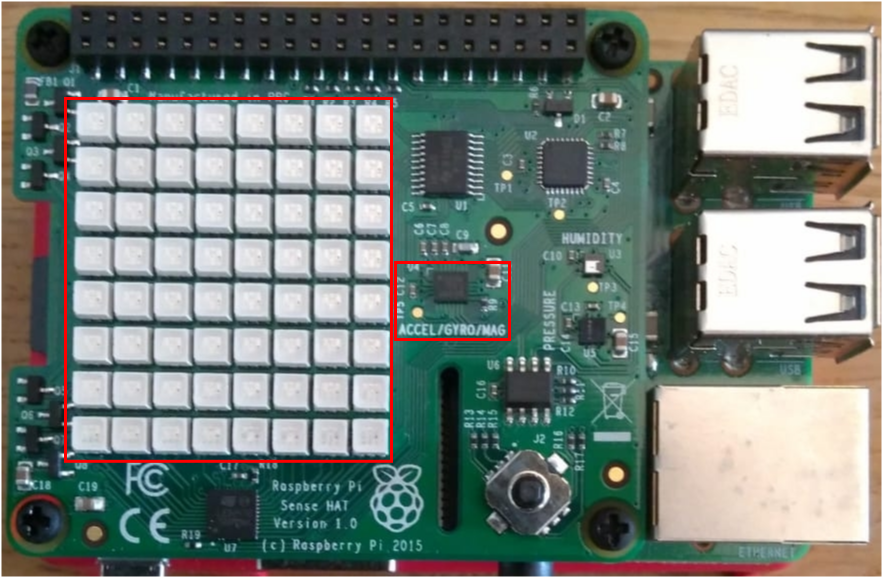
\includegraphics[width=0.6\textwidth]{Figures/results/sense_hat_self_dia.png}
    \caption{\gls{pi} with Sense HAT}
    \label{fig:sensehat}
\end{figure}

\begin{figure}[H]
    \centering
    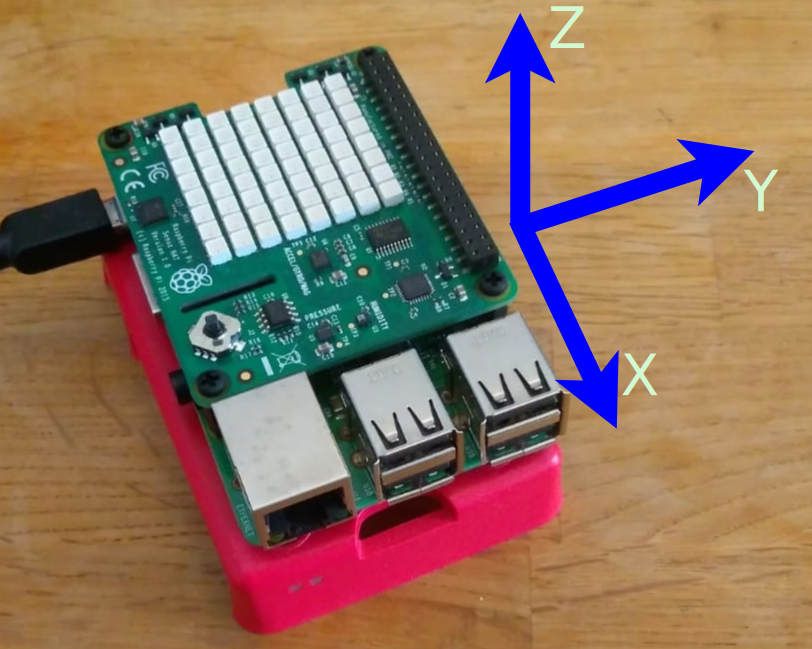
\includegraphics[width=0.6\textwidth]{Figures/results/pi_not_above.png}
    \caption{Axis of the IMU on the Sense HAT}
    \label{fig:imu_orientation}
\end{figure}

\subsection{Operating System}
\label{Operating System}
In our literature review in Section \ref{tOS} we saw that Linux distributions are often used in care robot systems, because ROS is a popular middleware and ROS runs best on Linux distributions. We choose to run a Linux distribution on the \gls{pi} of the safety module, because care robot Rose runs ROS as well, and the safety module needs to interact with care robot Rose. Specifically, we choose to run Raspbian, the Debian based Linux distribution for the \gls{pi}, as it is optimized for the \gls{pi}'s hardware (\cite{raspbian}).
\par
As was shortly mentioned in the description of the \gls{pi} in Section \ref{Main component} and as was elaborated in detail in the literature review of Section \ref{tOS}, the two prominent options for adding real-time support to Linux distributions are real-time Linux and the Xenomai framework. In Section \ref{tOS} we also saw a comparison between these two options, with the result that Xenomai performed better in terms of meeting hard real-time requirements. Now, for the prototype safety module that is developed in this research, we only aim for soft real-time performance. Still, further versions of the safety module will need to support hard-real-time performance, and we therefore choose to use the co-kernel setup of the Xenomai framework over Real-time Linux as our operating system.
\par 
% TODO: Gloss system call
As was shortly mentioned in Section \ref{tOS}, Xenomai provides various skins. These skins are interfaces to the real-time functionality that the Xenomai framework provides. We choose to work with the POSIX skin. The POSIX skin provides the functionality of the Xenomai framework through the interface of a subset of POSIX system calls. The following services are provided (\cite{posix_xenomai}):

\begin{itemize}\label{posix_wrapped}
    \item Clocks and timers
    \item Condition variables
    \item Message queues
    \item Mutual exclusion 
    \item Process scheduling 
    \item Semaphores
    \item Thread management
    \item Scheduling management
\end{itemize}

These POSIX services are wrapped around with Xenomai versions of the calls. For example, if one calls the \mintinline{c}{pthread_create} function to create a new thread in the C programming language or the C++ programming language, what is actually called is a real-time implementation of the system call provided by the Xenomai framework.
\par
The reason we choose to work with the POSIX skin as opposed to other skins is that the POSIX skin avoids the need to rewrite device drivers written for standard, non-Xenomai Linux, as such device drivers often use the POSIX services given in the previous list. In our case, this avoids the need to rewrite the driver for the Sense HAT. Likewise, \acrshort{ros} is targeted for standard Linux and not Xenomai, so using the POSIX skin also avoids having to rewrite \acrshort{ros} services. Section \ref{Implementation} shows how we implemented the safety module using the Xenomai framework.
\\\\
We have built \acrshort{ros} for Raspbian and installed it on our system. For this research we will simulate interaction with care robot Rose and ROS and we will not use this installation, however. The reason we installed \acrshort{ros} nonetheless is to show the feasibility of using the system of the \gls{pi} using Raspbian with Xenomai, as a whole.
\par
Figure \ref{fig:stack} gives a high level overview of this system as a whole, visualised as a stack. On the bottom we have the \gls{pi} with the Sense HAT, this is our hardware. On top of that there are the Linux kernel and the Xenomai co-kernel, which run next to each other. Then there is Raspbian Buster, the operating system. All the way on top we see RTIMULib, Dezyne and \acrshort{ros}. RTIMULib is the library used to communicate with the Sense HAT. Dezyne is the modelling language we use, which uses its own runtime library. The use of Dezyne is elaborated in detail in Section \ref{Formal model of the behavior of the system}. The reason RTIMULib and \acrshort{ros} are shown on top, despite the fact that both communicate with the hardware of the bottom layer, is because RTIMULib and \acrshort{ros} are both libraries called from user space. We can say that anytime we want to access a hardware device in our program we traverse the stack from top to bottom.

\begin{figure}[H]
    \centering
    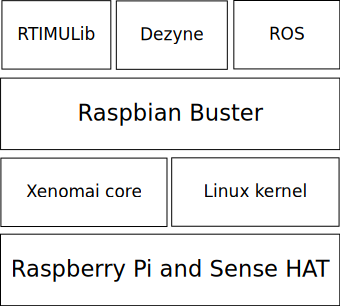
\includegraphics[width=0.5\textwidth]{Figures/results/os_environment_stack.png}
    \caption{Safety module system stack}
    \label{fig:stack}
\end{figure}


Let us look at a communication scheme of the system and how the Xenomai framework provides us with real-time operation of the safety module. In Figure \ref{fig:communication_scheme} an overview of the communication scheme of the system is given. On the left side we can see our program and the Xenomai core. These run in \textit{primary mode}, primary mode is the real-time domain; the part of the system that operates real-time, because it is governed by the Xenomai co-kernel. All scheduling of tasks in primary mode is handled by the Xenomai core. The Xenomai framework provides us with the ability to make a subset of system calls, the ones from the items listed in List \ref{posix_wrapped} without leaving primary mode. We depicted Dezyne to be inside our program, in primary mode. The code that Dezyne generates from the model is essentially the control loop of the safety module system. This control loops executes five checks, this is why there are five lines of communication going through the entire system in the overview of Figure \ref{fig:communication_scheme}. These checks are checks on five aspects of the robot: the kinetic energy, the rotational energy, the grip arm strength, both force and torque, and grip arm position. These checks are elaborated in detail in the subsequent Results sections. RTIMULib and ROS communicate with device drivers written for the standard Linux kernel, meaning they do not run in primary mode, but \textit{secondary mode}. Secondary mode is the non-real-time domain; the part of the system that does not operate in real-time and is governed by the standard Linux kernel. This brings us to a problem. Our program needs to communicate with these libraries, and therefore with these device drivers, but if it does so it would make a mode switch by moving from primary mode to secondary mode. One solution would be to reimplement all used device drivers to work with the Xenomai framework, so that they can run in primary mode. This solution, however, takes a lot of development time and research into how to convert standard linux drivers to real-time drivers. Luckily, Xenomai provides us with another solution: the use of XDDP sockets. XDDP sockets allow the part of the system running in primary mode to communicate data with the part of the system running in secondary mode, without the former leaving primary mode. This is good because now we can set up the system as follows. In primary mode the control loop runs in real-time governed by the Xenomai co-kernel. In secondary mode, threads retrieving data from the sensors are running and provide their data on the XDDP socket, which can then be read by the threads of the program running in primary mode. This set up fixes the problem of our control loop needing to leave primary mode to access sensor data. However, now, there is another problem hiding in the background. What should we do when the sensor data is not provided by the non-real-time thread when a real-time thread requires it? We go into more detail on this problem in Section \ref{Implementation}, but essentially the real-time checks just keep going regardless of whether there is data provided by the non-real-threads. That is to say, the checks do not block if there is no data available.

\begin{figure}[H]
    \centering
    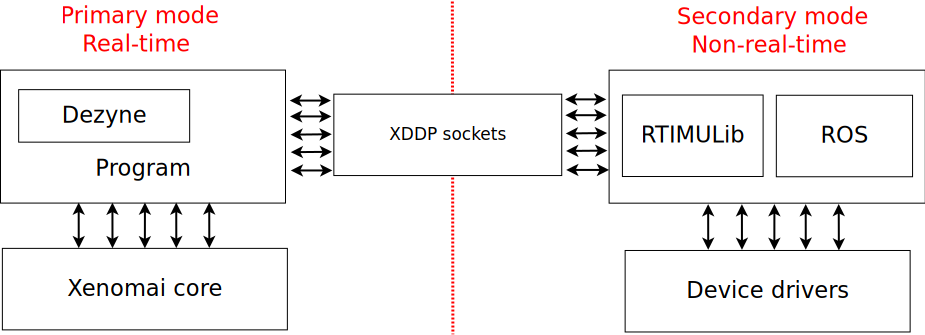
\includegraphics[width=\textwidth]{Figures/results/communication_scheme.png}
    \caption{Distinction between primary mode and secondary mode}
    \label{fig:communication_scheme}
\end{figure}

\newpage
\section{Retrieving and Using Sensor Data}
\label{Retrieving and Using Sensor Data}
In this section we elaborate our results on how to retrieve sensor data and use this data to check whether the safety module has performed any unsafe actions.
\par
In Section \ref{Assignment specification} we defined unsafe behaviour as behavior that could result in injury to humans or damage to the environment by collision, clamping or pinching of the care robot with an object or human. The goal of the safety module is to provide a second layer of safety checks upon the already existing safety checks by the care robot itself. In Section \ref{Safety in care robots} we explored how existing research measures safety in service robots. We implement a rudimentary form of some of these safety checks by looking at five aspects of the care robot. These are: its kinetic energy, its rotational energy, its grip arm force and torque and its grip arm's position. These aspects were given on the Risk Analysis for additional safety measures of robot Rose (\cite{risk_analysis_additional}).

\subsection{Sensors on the safety module}
The sensors of the Sense HAT of the safety module are used to check the kinetic energy and rotational energy of the robot. The safety module is attached to the care robot, and should be attached in a way such that the x-axis (see Figure \ref{fig:imu_orientation}) points forward; parallel to the front of robot Rose.
\par
We make use of the RTIMULib library, an open-source library that provides us an application programming interface (API) to interact with the accelerometer, gyroscope and magnetometer of the LSM91DS1, the inertial measurement unit of the Sense HAT (\cite{rtimulib}). With the use of a Kalman-filter the library provides fused data of the accelerometer, gyroscope and magnetometer. Kalman-filtering is a technique to provide an accurate measure of, in our case, the angular orientation of the safety module.

\subsection{Kinetic energy}
\label{Kinetic energy}
First we will look at the aspect of kinetic energy. In Newtonian mechanics, kinetic energy is defined as follows:

\begin{equation} \label{eq:ke}
    E_k = \frac{1}{2}mv^2
\end{equation}

where $m$ is the mass of the object undergoing linear translation and $v$ the velocity of the object undergoing linear translation. Robot Rose's mass is $95kg$ (\cite{rose_specification}), the \gls{pi}'s mass is $45g$ (\cite{raspberry_pi_weight}) and the Sense HAT's mass is $20g$ (own measurement). That gives us $m = m_{tot} = 95.065kg$. Velocity we do not measure directly, instead we measure the acceleration using the accelerometer on the Sense HAT. To obtain velocity $\vec{v}$ from acceleration $\vec{a}$, we numerically integrate $\vec{a}$ using the following equation:

\begin{equation} \label{eq:trapezoidal_rule}
    \vec{v} = \int_{t_0}^{t_f} \vec{a}\ dt \approx \sum_{t=t_0}^{t_f-1} \frac{\vec{a}(t) + \vec{a}(t+1)}{2}\Delta t
\end{equation}

where $t_0$ is the initial time, $t_f$ is the final time and $\Delta t$ is a small change in time. Equation \ref{eq:trapezoidal_rule} is called the \textit{trapezoidal rule}. For smaller $\Delta t$ the approximation becomes more accurate. We have set $\Delta t$ such that the time taken to sample the acceleration is a multiple of the recommended poll interval of the IMU as given by RTIMULib.
\par
Various sources report the occurrence of drift error due to sensor noise by use of integration to obtain velocity from acceleration (\cite{chrobotics}) (\cite{googletechtalks}) (\cite{Woodman07anintroduction_oliver}). However, we can still use this method of determining velocity for our purposes, for the obtained velocity is accurate enough to determine kinetic energy and we discard the value of velocity after determining the kinetic energy gained from it. Every time we calculate the kinetic energy, we do so by obtaining the kinetic energy that is gained from the change in acceleration. Our error does not get increasingly worse, because we only measure changes in acceleration and do not take into account the velocity the robot may already have.
\par
A subtle, but important point that follows from this, is that we do not actually measure the kinetic energy of the robot, but the change in kinetic energy. Furthermore, with discarding the previous value of velocity we mean we set the initial velocity to be zero every time we want to calculate the kinetic energy. The result is that the following equation holds:
\\\\

\begin{equation} \label{eq:change_ke}
    \Delta E_k = \frac{1}{2}m(\Delta v)^2 \implies \Delta E_k = \frac{1}{2}mv^2,\quad if\ \vec{v_i} = 0
\end{equation}

where $\Delta v$ is the change in velocity and $\vec{v_i}$ is the initial velocity. $\Delta v$ is not depicted as a vector here because squaring $\Delta v$ eliminates the sign of the velocity. In fact, as we only use the velocity to calculate kinetic energy, we actually only need to obtain the speed. Still, we obtain the velocity for scalability and in case someone wishes to do calculations with velocity in the future. 
\par
Excessive change in kinetic energy will make the robot injure a human or damage an object upon collision, which we defined as a form of unsafe behavior. To avoid this, the obtained change in kinetic energy is compared to the maximum allowed change in kinetic energy. For our purposes, this maximum allowed change in kinetic energy is the same for every situation. The maximum allowed change in kinetic energy is given as input to the safety module either in an input file or as command line argument. The maximum kinetic energy threshold value is not determined by us, but by the company or organisation who employs the safety module, who has tested and determined an appropriate value for this variable. We have chosen a value that most clearly demonstrates the use of the check on kinetic energy.

\subsection{Rotational energy}
\label{Rotational energy}
The rotational energy is determined analogous to the kinetic energy, but using angular variables instead, and we calculate the actual rotational energy, not the change in rotational energy. The rotational energy is calculated using the following equation:

\begin{equation} \label{eq:rot_energy}
    %\Delta E_{rot} = \frac{1}{2}I(\Delta\omega)^2 \implies \Delta E_{rot} = \frac{1}{2}I\omega^2,\quad if\ \vec{\omega_i} = 0
    E_{rot} = \frac{1}{2}I\omega^2
\end{equation}

where $I$ is the moment of inertia and $\omega$ is the angular velocity. For $I$ we approximate the robot as if it were a solid cylindrical object. $I$ can then be calculated as follows:

\begin{equation}
    I = \frac{1}{2}mR^2
\end{equation}

where $m$ is the mass of the robot and $R$ the radius of the robot. $R$ we approximate to be 1 meter, taking the scenario into account where Rose fully stretches her arm.
\par
The fused accelerometer, gyroscope and magnetometer data gives us an accurate measure of the angular displacement $\vec{\theta}$ of the safety module. With $\vec{\theta}$ we can calculate the angular velocity $\vec{\omega}$ using numerical differentiation as follows:

\begin{equation}
    \vec{\omega} = \frac{d\vec{\theta}}{dt} \approx \frac{\Delta\vec{\theta}}{\Delta t} = \frac{\vec{\theta}(t + \Delta t ) - \vec{\theta}(t)}{\Delta t}
\end{equation}

Here $\Delta t$ is a small change in time, which we set to be a multiple of the poll rate of the IMU, just like with $\Delta t$ used in the calculation of the linear velocity for the kinetic energy.
\par
Excessive rotational energy will cause the linear momentum of the robot to be too great when the robot makes a turn, which can result in damage to the environment or injury to humans. Therefore, just like with kinetic energy, the rotational energy is compared to a maximum allowed value which is given in an input file or command line argument.

\subsection{Sensors on robot Rose}
Ultimately, Rose's arm sensors will be used to retrieve the strength and position of the arm. These values are received from \acrshort{ros}. ROS provides a publisher-subscriber type of pattern in which a subscriber can listen on a \textit{topic} on which the publisher publishes data. In our case the subscriber would be the safety module and the publisher would be Rose. Topics in ROS are collections of messages concerning a particular subject, where a message is the means of communication of data in \acrshort{ros} (\cite{agitr}).
\par
Currently we use generated values from within the safety module itself and do not communicate with robot Rose through \acrshort{ros}.

\subsection{Force and torque}
Strength can be expressed with two different kind of forces. One force is the linear force of the arm against an object, the other is a rotational force, commonly called \textit{torque}, that is used to grab an object. We need not calculate the force and torque like we did with kinetic energy and rotation energy, because ultimately care robot Rose provides these values through \acrshort{ros}.
\par
Excessive force can cause the arm to clamp with an object, and excessive torque can cause the arm to pinch an object. Both are cases we want to avoid. We, therefore, just like with kinetic energy and rotational energy, set a maximum allowed value for the force and torque, which should not be exceeded.

\subsection{Position}
The last check on unsafe behavior concerns the arm position of the robot. When the robot is moving, the arm should be in a folded position. This means it is not stretched, and in a position that it can do the least amount of harm. This value, too, is ultimately provided by Rose through \acrshort{ros}, and need not be calculated by the safety module.

\subsection{When the result of a check gives unsafe behavior}
\label{When the result of a check gives unsafe behavior}
What should we do when a check is executed and the maximum allowed value for the kinetic energy, rotational energy, force, torque is exceeded, or the arm is not folded when the robot is moving? 
These are the situations we call unsafe behavior. In such a case, the LED matrix receives a signal to turn red. On default, the LED matrix is low. When a check is executed and the result of the check is that there is no unsafe behavior, the LED matrix receives a signal to turn blue. Only when the result is that there is unsafe behavior does the LED matrix receive a signal to turn red. Checks are executed in sequence. An important point to note here is that situations exist, where, for example, the result of the first of the five checks gives unsafe behavior, while the subsequent checks give safe behavior. In such a case, the LED matrix should turn red after the first check, and stay red after the subsequent checks. This is because unsafe behavior of one safety check is not supposed to be overridden with safe behavior of another safety check. We therefore specify that once the result of a check gives unsafe behavior, the LED stays red until an acknowledge action is executed. This acknowledge action, among the other actions of the system, is elaborated in Section \ref{Formal model of the behavior of the system}.

\newpage
\section{Modelling of the safety module}
\label{Formal model of the behavior of the system}
In this section, we elaborate our results on the modelling of the safety module. We present a formal model of the behavior of the safety module made with the modelling toolset \textit{Dezyne}. In this section, we present the most important elements of the model. An in depth exploration of all components of the model can be found in Appendix \ref{In depth elaboration of Dezyne in the safety module}. In additional to that, some auxiliary models can be found in Appendix \ref{Additional Models}, and all models, in general, can be found on \href{https://github.com/Yousousen/safety-module-for-care-robot-rose.git}{our GitHub repository}.
\\\\

%The basics of the Dezyne toolset and modelling language were elaborated extensively in Section \ref{The Dezyne toolset and the Dezyne modelling language}. There we also explained what Dezyne's behavior verification does. In short, it checks the system on the occurrence of race conditions, deadlocks, livelocks, mismatches between specification and implementation and concepts related to deterministic behavior of the system. A prototype of the language has also the capability to check the system on functional behavior. That is to say, it checks whether a system, after executing a set of actions, is in the expected system state. If it is not, this will be output as a functional verification error. In this section, we will present our formal behavior model of the safety module. We will first present an overview of the system, which shows us all components of the system, then we will work from inside out, going through the individual components of the system.


\subsection{System overview}
\label{System overview}
Let us first look at the system overview, which is shown in Figure \ref{fig:safety_module_system_view}.

\par
In Figure \ref{fig:safety_module_system_view} we can see the hierarchy of all components that are implemented in Dezyne. On top there is the \texttt{Controller}. The \texttt{Controller} governs the entire system, and executes safety checks in sequence. These checks are checks on kinetic energy, rotational energy, force of the grip arm, torque of the grip arm and position of the grip arm, as we established in Section \ref{Retrieving and Using Sensor Data}. Each check is implemented like an element in a linked list. A linked list is a data structure in which each element of the list points to the next element. So, in this case, each check points to and executes the next check. This provides the system a level of abstraction and generality. When one wishes to add a new check to the system, one does not need to make changes to the \texttt{Controller}, and the only thing that needs to be changed is the pointer that points to the next check at the location in the list one wishes to add the new check. No changes need to be made to any other aspect of the system logic outside of the added check itself.
\par
Every check returns a value, \texttt{Behavior.Safe} or \texttt{Behavior.Unsafe}, which indicates whether the executed action of the care robot results in safe or unsafe behavior. 
%\par
%The model can be simulated, which shows a trace of a system along a certain path of actions which results in a sequence diagram, as we will see in subsequent subsections.
%In such a simulation we can choose whether a particular check returns safe or unsafe behavior ourselves. In the real non-simulated system, however, the system will return safe or unsafe behavior based on whether the retrieved value of the quantity the check examines exceeds the maximum allowed value, or, in the case of the arm position, whether the arm is or is not in folded position. 
\par
% Ref to SQ 4
In Figure \ref{fig:safety_module_system_view} we can see blue squares going into and out of components. These are called \textit{ports}. These ports play a role in the generation of source code from Dezyne models. An example of the generation of source code is given in Section \ref{The Dezyne toolset and the Dezyne modelling language} of Appendix \ref{Short introduction to the Dezyne toolset}. Ports on the the edges of the system need to be bound in implementation code to generated source code. With implementation code we mean the C++ code of the safety module program that will run on the \gls{pi}. The single port at the top of the system view denotes the \texttt{Controller} port that we may intract with to bind to a function in implementation code in order to execute the dezyne system, or, in other words, the safety checks. The six ports at the bottom are ports that also need to be bound in implementation code, but these are executed by Dezyne internally, that is, we assign a function for Dezyne to execute by binding these ports. The binding of ports is elaborated in Section \ref{Binding Dezyne events to functions}.
\par
%In Section \ref{The Dezyne toolset and the Dezyne modelling language} we mentioned how a Dezyne model consists of interfaces and components, where interfaces specify the behavior a component should conform with and which events or actions a component can execute.% It should be noted that the system view of Figure \ref{fig:safety_module_system_view} only shows us the components of the system. It does not show us interfaces of components. This is because an interface is a specification and not an actual implementation of an aspect of the system. Interfaces are still aspects of the system that can be verified on behavior, however, as we will see when we examine the behavior of \texttt{ILEDControl}, an interface that concerns itself with turning the LED matrix blue in case of safe behavior of the care robot and red in case of unsafe behavior of the care robot.
\begin{figure}[H]
    \centering
    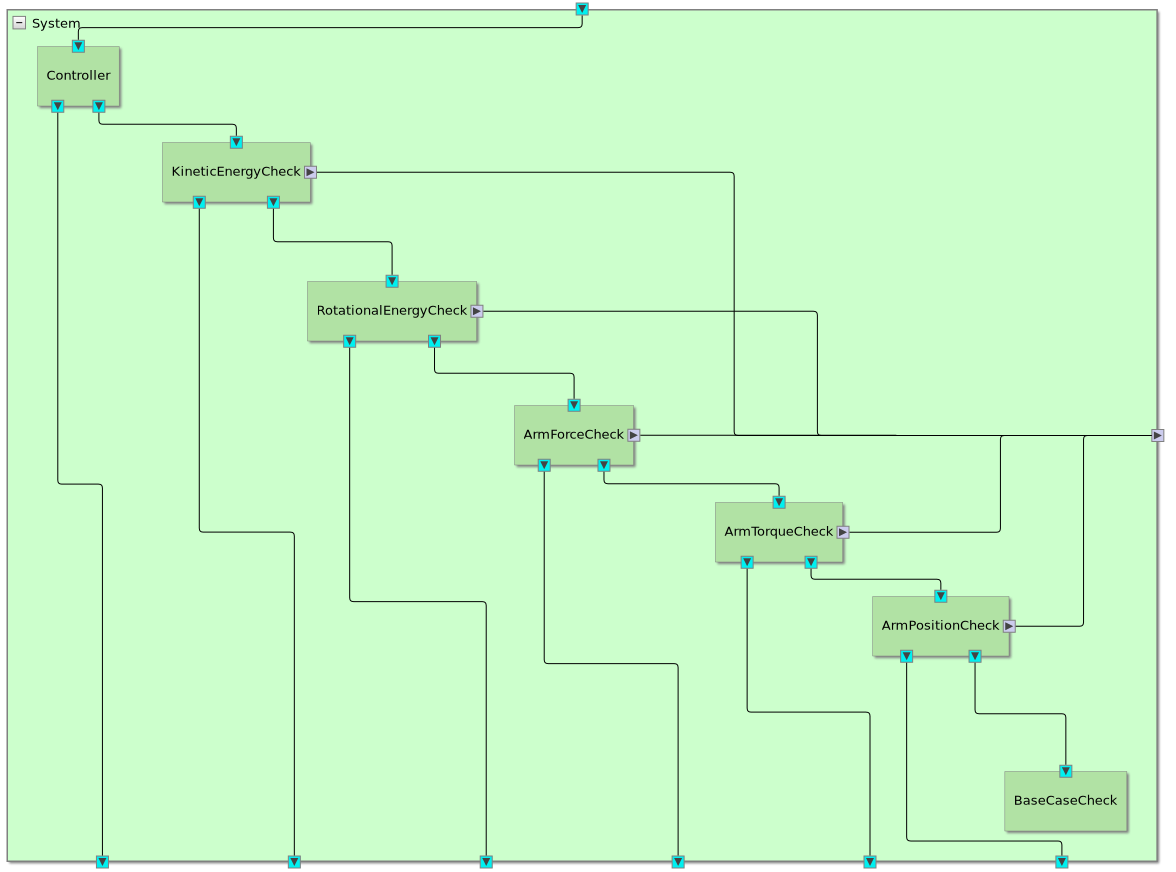
\includegraphics[width=\textwidth]{Figures/results/modelling_figures/system_view/system_view.png}
    \caption{System view of the safety module system}
    \label{fig:safety_module_system_view}
\end{figure}

% ref to section SQ4
\subsection{The IController interface}
\label{secIController}
Dezyne models consist of interfaces and components, where interfaces specify the behavior a component should conform to and which events or actions a component can execute. Thus, the \texttt{IController} interface specifies the behavior the \texttt{Controller} component should conform to and its actions. In this section we will elaborate the \texttt{IController} interface and in the next section we will elaborate the \texttt{Controller} component. The controller is the component that governs the safety module system, it starts the check sequence and controls the LED matrix.
\par
In Figure \ref{fig:IController_state_chart}, the state chart of \texttt{IController} is given. Here we see that when the \texttt{initialise} event fires, the \texttt{initialise\_imu}, \texttt{initiliase\_mutexes} and\\\texttt{initialise\_semaphores} are called and the system jumps from the \texttt{Idle} to the \texttt{Operating} state. Calling \texttt{initialise\_imu}, \texttt{initiliase\_mutexes} and \texttt{initialise\_semaphores} on the \texttt{initialise} event ensures that the IMU, mutexes and semaphores used by the safety module are always properly initialised before the system will execute its control loop in the \texttt{Operating} state. The safety module makes use of mutexes and semaphores because the implementation is multithreaded. In a similar manner as \texttt{initialise}, when the \texttt{destruct} event fires, the \texttt{destruct\_mutexes} and \texttt{destruct\_semaphores} are called. The IMU need not be explicitly destructed. These destruct actions are not supposed to execute, however, as the safety module is expected to run indefinitely in the \texttt{Operating} state, or at least until Rose shuts down.
\par
In the \texttt{Operating}, state \texttt{do\_checks} calls the first check of the linked list of checks. \texttt{do\_checks} is shown twice in Figure \ref{fig:IController_state_chart}, because the interface specifies that \texttt{do\_checks} either returns \texttt{UnsafeTriggerered.Yes} or \texttt{UnsafeTriggered.No}. The notions of\\\texttt{UnsafeTriggerered.Yes} and \texttt{UnsafeTriggered.No} are used to monitor whether one or more of the checks returned unsafe behavior.
\par
To explain the controller further, we will look at the \texttt{Controller} component.

\begin{figure}[H]
    \centering
    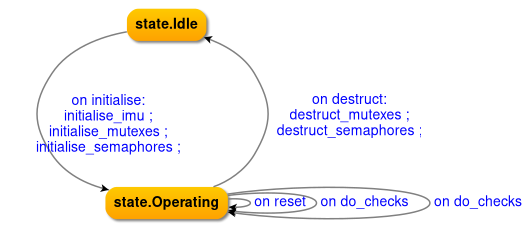
\includegraphics[width=0.8\textwidth]{Figures/results/modelling_figures/IController/IController_state_chart.png}
    \caption{State chart of IController}
    \label{fig:IController_state_chart}
\end{figure}

\subsection{The Controller component}
\label{secController}
In Figure \ref{fig:controll_event_table} the event table of the controller is shown. We have already elaborated \texttt{initialise} and \texttt{destruct} in the controller its interface. In addition to the behavior specified by its interface, the controller also calls \texttt{initialise\_framebuffer} when the \texttt{initialise} events fires as well as \texttt{destruct\_framebuffer} when the \texttt{destruct} events fires. Because the event table omits an important conditional in the code column, we will refer to the actual Dezyne code we used to create the model for the \texttt{do\_checks} event, which is listed in Code \ref{mdo_checks}. For the \texttt{reset} event, we refer to Figure \ref{fig:controll_event_table}.
\par
Let us first look at \texttt{do\_checks}. Upon entering the \texttt{do\_checks} event, we call the \texttt{do\_check} event of \texttt{iHead}. \texttt{iHead} always points to the first check in the list. On lines 5 to 7 there is an if statement that is entered when the result of \texttt{iHead.do\_check} is \texttt{Behavior.Unsafe}. When will the result of \texttt{iHead.do\_check} be \texttt{Behavior.Unsafe}? When we execute a check, the check will internally call \texttt{do\_check} of the next check. So, if we start at the Controller, it will call the \texttt{do\_check} of\\\texttt{KineticEnergyCheck}, \texttt{KineticEnergyCheck}'s \texttt{do\_check} will call \texttt{RotationalEnergy}'s \texttt{do\_check}, \texttt{RotationalEnergy}'s \texttt{do\_check} will call \texttt{GripArmForce}'s \texttt{do\_check}, etc. This will be done all the way to \texttt{BaseCaseCheck}'s \texttt{do\_check}. \texttt{BaseCaseCheck}'s \texttt{do\_check} always returns \texttt{Behavior.Safe}. Every check executes a boolean AND function on its own and next check's result, returning \texttt{Behavior.Unsafe} when either one or both of the checks reply \texttt{Behavior.Unsafe}. Since the recursion stops at \texttt{BaseCaseCheck}, we can traverse the linked list back up again, finishing all \texttt{do\_check} calls. Along the way back up, every check will perform the boolean AND function with the subsequently executed check. This means that, ultimately, the result of \texttt{iHead.do\_check} in the controller is the result of all boolean ANDs from all checks that were called on the way through the linked list. This implies that the result of \texttt{iHead.do\_check} in the controller is \texttt{Behavior.Unsafe} as soon as one or more of the checks result in \texttt{Behavior.Unsafe}.
\par
If the result of \texttt{iHead.do\_check} in the controller is \texttt{Behavior.Unsafe}, we enter the if statement on Line 5 of Listing \ref{mdo_checks}. Since the safety module has detected unsafe behavior, we will now instruct \texttt{iLEDControl} to light the LED matrix red. Signalling unsafe behavior like this is the safety module's most important task, so it has the highest priority in the system.
\par
On Line 7 of Listing \ref{mdo_checks}, we set \texttt{unsafe\_acknowledged}, a boolean variable, to \texttt{false}. The boolean variable \texttt{unsafe\_acknowledged} denotes whether the operator of Rose, or any system that monitors Rose for that matter, has acknowledged or recognized that unsafe behavior has taken place. On Lines 11 to 16, we can see that the controller replies \texttt{UnsafeTriggerd.Yes} if \texttt{unsafe\_acknowledged} has the value of \texttt{false} and that the controller replies \texttt{UnsafeTriggered.No} if \texttt{unsafe\_acknowledged} has the value of \texttt{true}. {unsafe\_acknowledged} is the mechanism to prevent one to override a red LED with a blue LED. It is for this reason that we can only set the LED to blue when \texttt{unsafe\_acknowledged} has the value of \texttt{true}, for so long no one or nothing has acknowledged that the robot has performed unsafe behavior the LED matrix should stay red. In Figure \ref{fig:controll_event_table}, we can see that the \texttt{reset} event sets \texttt{unsafe\_acknowledged} to the value of \texttt{true} and that it instructs the \texttt{iLEDControl} to reset the LED matrix. The \texttt{reset} action corresponds to the operator of the robot acknowledging the unsafe behavior. \texttt{reset} is the only action in the system that can reset the LED matrix and that can acknowledge unsafe behavior. The notions of \texttt{UnsafeTriggered.Yes} and \texttt{UnsafeTriggered.No} of Listing \ref{mdo_checks} are related to this. So long as the unsafe behavior is not acknowledged, the controller will return \texttt{UnsafeTriggered.Yes}. It is only if no unsafe behavior has yet been detected or if the unsafe behavior has been acknowledged by the operator of the robot that the controller's \texttt{do\_check} event will return \texttt{Unsafe.Triggered.No}.

 \begin{figure}[H]
     \centering
     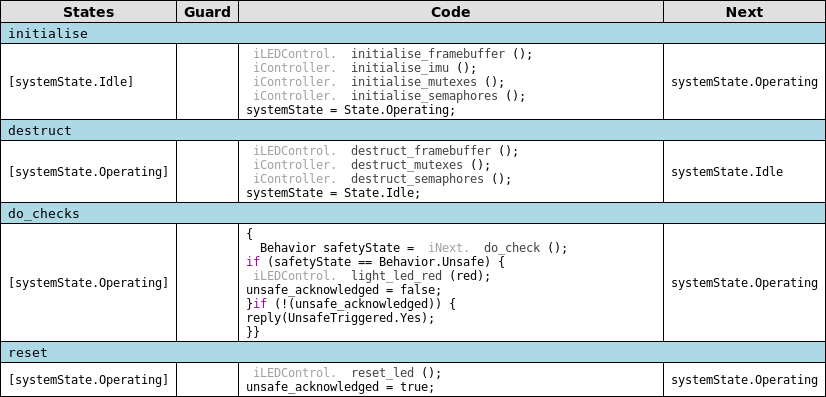
\includegraphics[width=\textwidth]{Figures/results/modelling_figures/Controller/Controller_event_table.png}
     \caption{Event table of \texttt{Controller}}
     \label{fig:controll_event_table}
 \end{figure}
 
\begin{listing}[!ht]
\begin{minted}[mathescape,
               numbersep=5pt,
               frame=lines,
               framesep=5mm,
               linenos]{haskell}
on iController.do_checks(): {
    Behavior safetyState = iHead.do_check();
	
    if (safetyState == Behavior.Unsafe) {
        iLEDControl.light_led_red(red);
        unsafe_acknowledged = false;
    } else if(unsafe_acknowledged) {
        iLEDControl.light_led_blue(blue);
    }
    if(!unsafe_acknowledged) {
        reply(UnsafeTriggered.Yes);
    }
    else {
        reply(UnsafeTriggered.No);
    }
}

 \end{minted} 
\caption{\texttt{on iController.do\_checks()} definition} \label{mdo_checks}
 \end{listing} 
 
In the verification results on the \texttt{Controller} component shown in Figure \ref{fig:controll_verif}, we see that to verify a component, we first need to verify and ensure that none of the interfaces it implements or uses contains verification errors.
 
\begin{figure}[H]
    \centering
    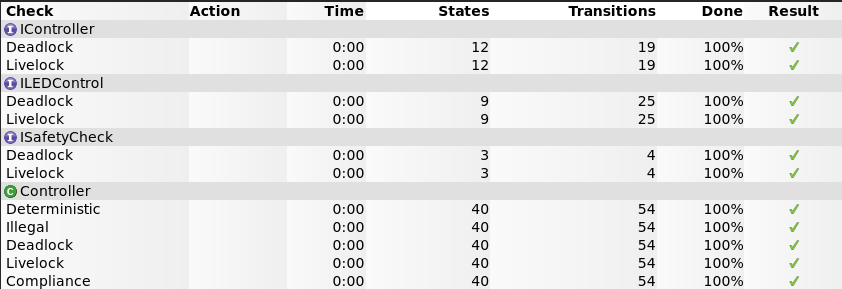
\includegraphics[width=\textwidth]{Figures/results/modelling_figures/Controller/Controller_verification.png}
    \caption{Verification results for \texttt{Controller}}
    \label{fig:controll_verif}
\end{figure}

Figure \ref{fig:controller_seq} shows a sequence diagram of the Controller. Here we first execute the \texttt{initialise} action to initialise the system, then we execute \texttt{do\_checks} multiple times. This sequence diagram does not show us a completely recursive trace through all the safety checks, sadly. This is a result of making the model generic by using a linked list like data structure for the checks. Because we simulate the model to create a sequence diagram of the controller, we get to choose what value \texttt{iNext.do\_check} returns, and the system need not recursively traverse all checks to determine the correct return value for \texttt{iNext.do\_check}. Note, however, that the operation of a simulation like this is different from what the verifier does; the verifier \textit{does} need to recursively traverse through the checks. It furthermore needs to traverse any particular sequence of events as to ensure there are no errors hiding in a particular path through the system.
\par
We added a sequence diagram of a less generic, earlier version of the Controller to show how a sequence diagram looks that shows multiple checks being executed in sequence to Appendix \ref{Additional Models}. This sequence diagram can be found in Section \ref{aController}. This sequence diagram uses old naming conventions that are not used anymore.


\begin{figure}[H]
    \centering
    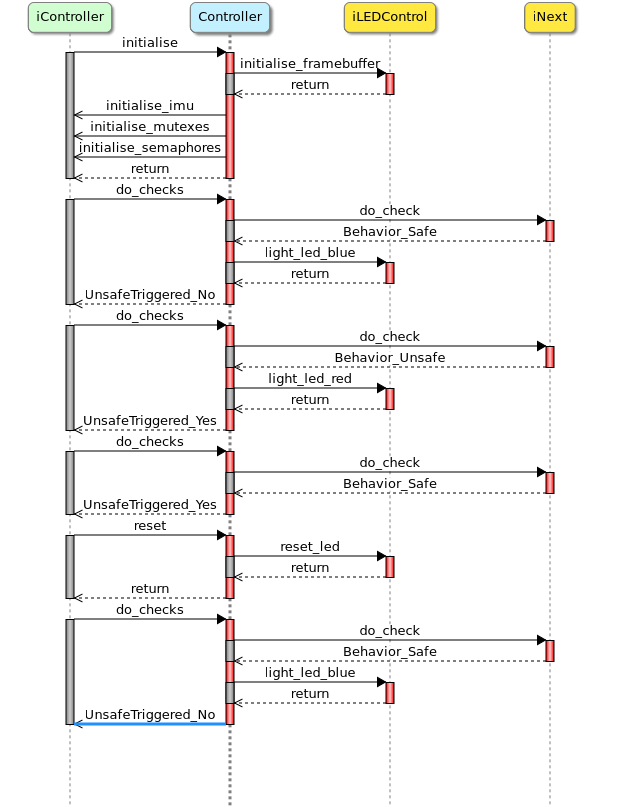
\includegraphics[width=\textwidth]{Figures/results/modelling_figures/Controller/Controller_seq.png}
    \caption{Sequence diagram of the controller}
    \label{fig:controller_seq}
\end{figure}


\newpage
\section{Implementation}
\label{Implementation}
In this section, we will elaborate the implementation of the safety module. We avoid showing source-code and try to elaborate the results by the use of figures and diagrams to make the text comprehensible to a broader public.

\subsection{Multithreaded nature of the safety module}
\label{Multithreaded nature of the safety module}
% TODO: Gloss UML
%In this section we present two models that are used to model aspects of the safety module system that are not captured by Dezyne. The first model shows the various threads of the safety module. The second model shows a UML class diagram showing the representation of care robot Rose the safety module utlizes.

In this section, we present various models regarding the multithreaded nature of the safety module. In Dezyne we did not module the system as a set of threads; instead in the Dezyne model there is just one thread that executes checks in a sequential manner, as we mentioned in Section \ref{Formal model of the behavior of the system}. One might wonder what gain a system has from being multithreaded if the control loop, the essence of the system, executes checks in a sequential manner. This is what we would like to elaborate in this section.
\par
To see the idea behind the multithreaded system with a sequential control loop let us consider the overview of threads in the safety module system in Figure \ref{fig:threads_overview}. On top, we see \texttt{rt\_<task>} and \texttt{nrt\_<task>}. These do not denote threads, but the general naming convention for the threads of the system. \texttt{<task>} denotes the specific task a thread executes. Below the right arrow, we see that two of these tasks are to light the LED and to reset the LED. Here we see both two threads prefixed with \texttt{rt\_} and two threads prefixed with \texttt{nrt\_}. \texttt{rt} stands for real-time and \texttt{nrt} stands for non-real-time. These threads thus denote real-time and non-real-time threads. Real-time threads are supposed to run in primary mode and should not make a mode switch to secondary mode, as to ensure that they are only governed by the Xenomai co-kernel and not by the standard Linux kernel. Why would a thread running in primary mode be a real-time thread? This is because the Xenomai kernel handles all time critical activities, and has priority over the standard Linux kernel. All we have to do is to make sure that the tasks that require real-time operation stay in primary mode. In contrast to the real-time threads, the non-real-time threads are allowed to be in secondary mode. A mode switch to secondary mode is made when the thread makes a kernel call to the standard Linux driver. This happens when a system call is made that is not wrapped with a real-time version by the Xenomai framework. In Section \ref{Operating System} we showed that a subset of POSIX system calls are wrapped by the Xenomai framework. A thread will make a mode switch to secondary mode when it makes a call to the IMU or to \acrshort{ros}. This is why only non-real-time threads are allowed to communicate with drivers like the IMU and ROS. One might wonder how sensor data can then be obtained by a real-time thread without leaving primary mode. We answered this question briefly in Section \ref{Operating System}, real-time threads can receive sensor data by use of XDDP sockets. We will look at this in more depth later this section.
\par
In the middle of Figure \ref{fig:threads_overview}, on the left side of the arrow, we have \texttt{rt\_sample\_<quantity>}, \texttt{rt\_retrieve\_quantity} and \texttt{nrt\_retrieve<quantity>}. These are threads concerning the sampling and retrieval of a quantity. Here \texttt{<quantity>} refers to the quantity measured by the five safety checks. So \texttt{<quantity>} refers to acceleration, angular displacement, force, torque or position. These threads run periodically, in contrast to the LED threads, which do not run periodically and are initiated by the main thread. The main thread is caleld \texttt{sm} and we can see it on the far left of Figure \ref{fig:threads_overview}. Below that we see the check thread, \texttt{rt\_do\_checks}, which is essentially our Dezyne system running indefinitely, sequentially going through the five checks.

\begin{figure}[H]
    \centering
    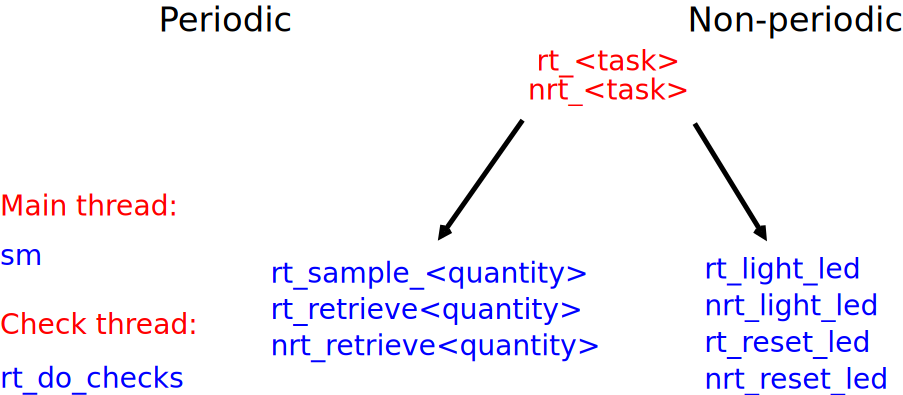
\includegraphics[width=\textwidth]{Figures/results/modelling_figures/Threading/threads_overview.png}
    \caption{Overview of threads in the safety module}
    \label{fig:threads_overview}
\end{figure}

Let us take a closer look at the threads that concern themselves with the LED matrix. In Figure \ref{fig:led_threads} we have given a diagram highlighting the communication between the LED threads. At the top we see \texttt{dzn\_light\_led} and \texttt{dzn\_reset\_led}. These are in fact not threads; \texttt{dzn\_light\_led} and \texttt{dzn\_reset\_led} denote functions that are initiated from Dezyne by the main thread. \texttt{dzn\_light\_led} corresponds to a \texttt{light\_led\_blue} action or a \texttt{light\_led\_red} action and \texttt{dzn\_reset\_led} corresponds to a \texttt{reset\_led} action, all three which we have seen in the models of Dezyne. The \texttt{dzn} functions initiate a line of communication between threads up to the LED driver. Both lines of communication on the left side and on the right side have identical operation, differing only in their task, namely lighting the LED or resetting the LED. The \texttt{dzn} functions increment a semaphore, both have a semaphore respective for their task, which the \texttt{rt} threads decrement. The \texttt{rt} threads wait for the semaphore to be incremented before they do any work. The \texttt{rt} threads then write over XDDP sockets, also one respective for the task, which actuate the \texttt{nrt} threads to write to the LED driver. The XDDP sockets prevent the \texttt{rt} threads from making a mode switch to from primary mode to secondary mode, by tasking the \texttt{nrt} to do the writing to the LED driver instead. Thus, the \texttt{nrt} threads make a mode switch from primary mode to secondary mode, but this is not a problem, as this is what they are designed for. Both \texttt{nrt\_light\_led} and \texttt{nrt\_reset\_led} access the LED driver mutual exclusively.

\begin{figure}[H]
    \centering
    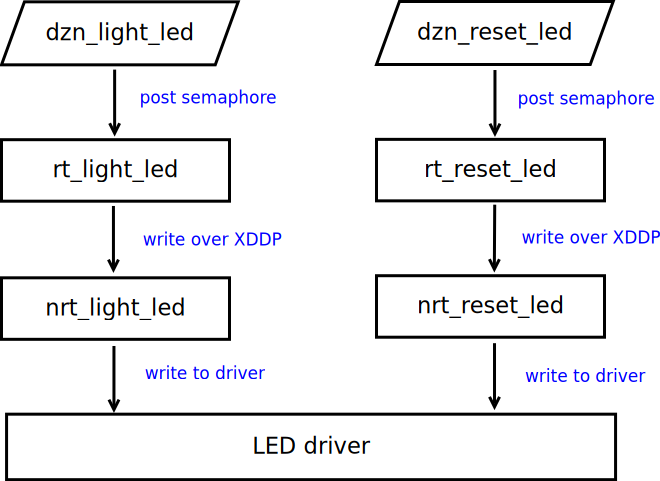
\includegraphics[width=0.8\textwidth]{Figures/results/modelling_figures/Threading/LED_threads.png}
    \caption{Communication between the LED threads}
    \label{fig:led_threads}
\end{figure}

In Figure \ref{fig:led_threads} we have seen one way how the multithreaded nature of the safety module manifests itself. To light the matrix or to reset the matrix the Dezyne loop of the main thread just increments semaphores, which does not take any significant time. It lets the \texttt{rt} and \texttt{nrt} threads do the actual work. The LED threads are the only threads in the system that are actuated by the main thread. The other threads of the system run periodically at a rate which is a multiple of the IMU poll rate, to provide a common factor of time between the threads.
\par
Let us now look at the communication between the \texttt{<quantity>} threads, which shows the other way how the multithreaded nature of the safety module manifests itself. In Figure \ref{fig:quantity_threads} we have given a diagram highlighting the communication between the \texttt{<quantity>} threads. Since \texttt{<quantity>} denotes acceleration, angular displacement, force, torque or position, this diagram implies that most threads of the system operate in a similar manner, differing only in the quantity they are involved with. Each thread in the diagram is involved with the same quantity, so there is no communication between threads that are involved with different quantities. In the top left of Figure \ref{fig:quantity_threads} we see \texttt{dzn\_retrieve\_<checked\_quantity>}, this is once again a function called from the main thread instead of a thread itself. The \texttt{dzn\_retrieve\_<checked\_quantity>} function is called from inside an executing safety check. In the figure, a distinction is made between \texttt{quantity} and \texttt{checked\_quantity}. The checked quantity is the quantity that is being checked by one of the five checks. For example, in the case of the kinetic energy check, the quantity is acceleration and the checked quantity is kinetic energy. In the case of the arm checks, the quantity and checked quantity are the same, for that what we receive from the sensors is also the safety metric. The \texttt{checked quantity} ellipse at the top right of the figure denotes a variable. This variable is read by the \texttt{dzn\_retrieve<checked\_quantity>} function and updated by the \texttt{rt\_sample\_<quantity>} thread, both in a thread-safe manner. The \texttt{rt\_sample\_<quantity>} thread samples the quantity in real-time. It retrieves the quantity from \texttt{rt\_retrieve<quantity>} over a socket connection between the two threads. The \texttt{rt\_retrieve<quantity>} thread retrieves the quantity from \texttt{nrt\_retrieve\_<quantity>}, which in turn retrieves the quantity from the driver. Here we see the same pattern as is used by the LED threads of Figure \ref{fig:led_threads}. A real-time thread communicates with a non-real-time thread over an XDDP socket so that it can stay in primary mode (if it did not stay in primary mode we would not have called it a real-time thread).
\par
There is a subtle point to make. For the arm force check, the arm torque check and the arm position check there is no \texttt{rt\_sample\_<quantity>} thread, because the quantity is the same as the checked quantity (e.g. the force check retrieves force from the driver and force is also the safety metric). The rest of the figure remains the same for these checks.

\begin{figure}[H]
    \centering
    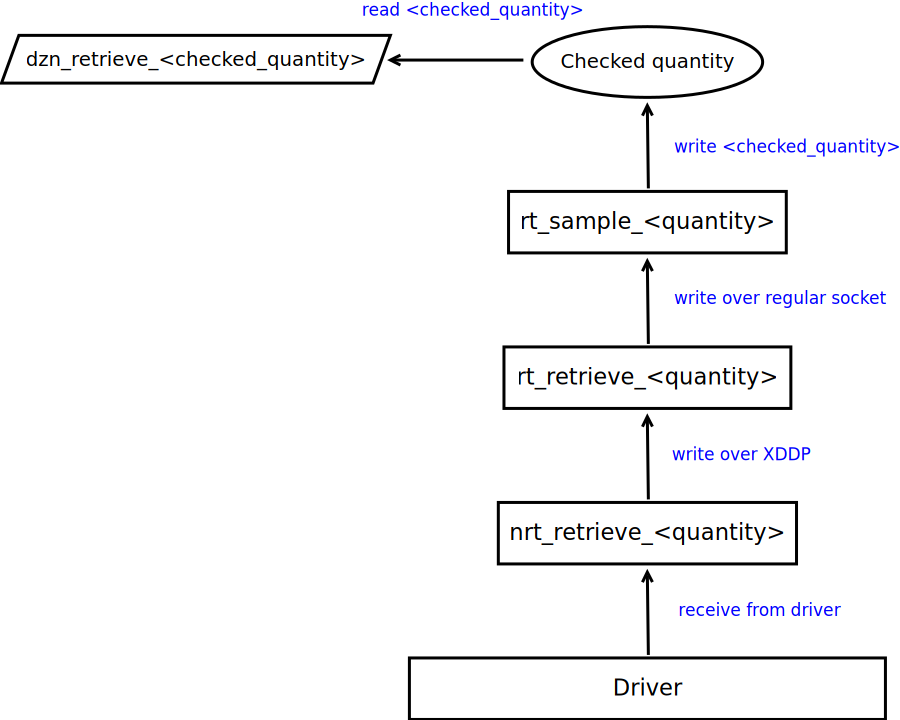
\includegraphics[width=0.9\textwidth]{Figures/results/modelling_figures/Threading/quantity_threads.png}
    \caption{Communication between \texttt{<quantity>} threads}
    \label{fig:quantity_threads}
\end{figure}

We have set up the communication between threads this way so that\\ \texttt{dzn\_retrieve\_<checked\_quantity>} need not do any work other than retrieving the checked quantity, which is a cheap operation in terms of time. The respective threads do the work of sampling and retrieving the quantity. Furthermore, the variable containing the checked quantity always has a value, so the \texttt{dzn\_retrieve\_<checked\_quantity>} need not block because no data is available. It is in this manner that the multithreaded nature of the safety module manifests itself while working with the sequential nature of the Dezyne control loop.


% note about absence of resolve.


\subsection{Binding and calling Dezyne events}
\label{Binding Dezyne events to functions}
In the previous Results sections we have mentioned the interaction of the Dezyne system with the rest of the safety module several times. It is now time to elaborate how exactly the transition is made from the formal model to implementation.
\par
In Section \ref{System overview}, we saw the System View of the safety module, shown in Figure \ref{fig:safety_module_system_view}. In that section, we talked about ports which are instances of interfaces that are found on the edges of the system. Some of these ports contain events that need to be bound to implementation code. After generating code from the Dezyne models, the binding of these edge ports to functions in the implementation code is essentially the step that needs to be taken to transition from design to implementation. The Dezyne runtime, which is imported in the implementation code, makes sure we bind every event that needs to be bound. Not all ports on the edges of the System View need to be bound to a function in the implementation, some need only be called from the implementation code. Which events need to be called and which events need to be bound is determined by the location of the ports in the System View. Ports on the top edge of the System View, from which we see only one in Figure \ref{System overview}, need to be called. The one port on top is the \texttt{Controller} port. Calling this port in implementation code will execute the control loop. The ports at the bottom of Figure \ref{System overview} all need to be bound to a function in implementation code. These ports on the bottom are the \texttt{Sensors} which contain the retrieve events. These retrieve events are bound to their respective \texttt{rt\_retrieve\_quantity} function. These functions are then executed as threads. on the right of the System View we see one gray port, this is the \texttt{Resolver}, responsible for translating values to Dezyne control logic. The \texttt{Resolver} is actually very similar to the \texttt{Sensor} ports at the bottom. It contains events that need to be bound in implementation code, just like the \texttt{Sensors}. The difference is that each sensor is implemented as a separate interface (there are five sensors, one for each checked quantity), while the resolver is one interface that contains all events required to resolve the values.

\subsection{Testing the safety module}
\label{Testing the safety module}
In this section we elaborate various tests on the real-time operation of the safety module.

\subsection{Latency tests}
\label{Latency tests}

In this section, we elaborate the latency tests we performed on the system. The latency of the system refers to the the time between a stimulus and the system's response. The latency tests were run with Xenomai's test suite program \texttt{latency}. In this section, two latency tests are shown. The first test shows the latency of the system without the safety module program running and the second test shows the latency of the system while running the safety module. All shown latency statistics have units of microseconds. Both tests schedule tasks with a period of $1000$ microseconds, the highest scheduling priority of $99$. The tests are both run for $20$ seconds. 
\par
Let us first look at the latency of the system without the safety module program running. This test is shown in Figure \ref{fig:lat_without_sm}. The elements that are of interest to us are the minimum latency, the average latency and the maximum latency, which are highlighted in that order in the red frame. The highlighted minimum latency and highlighted maximum latency are respectively the best and the worst latency of the system in the past $20$ seconds. The highlighted average latency is the average of the average latency of the system of the past $20$ seconds. We can see that for the system without the safety module program running, the minimum latency is $14.945$ microseconds, the average latency is $15.712$ microseconds and the maximum latency is $31.504$ microseconds. 
\par
If we then look at Figure \ref{fig:lat_with_sm}, the latency test with the safety module program running, we can see highlighted in the red frame that the minimum latency is $14.374$ microseconds, that the average latency is $21.281$ microseconds and that the maximum latency is $549.527$ microseconds. Thus, there is a slight increase in the average latency compared to the average latency shown in Figure \ref{fig:lat_without_sm}, and there is an increase by a factor of $~17$ for the maximum latency. Coincidentally, there is a slight decrease in the minimum latency. In both Figure \ref{fig:lat_without_sm} and Figure \ref{fig:lat_with_sm}, in the fourth column from the right, we can see that the test tasks have no deadline overruns.
\par
Sadly, our safety module's own threads could not be used to test the latency of the system (the safety module threads are only used to put a load on a system); we instead are limited to using test tasks. However, Section \ref{Mode switches and other statistics} shows other interesting statistics that are run on the safety module's own threads.
% Interpret this in the conclusion.

\begin{figure}[H]
    \centering
    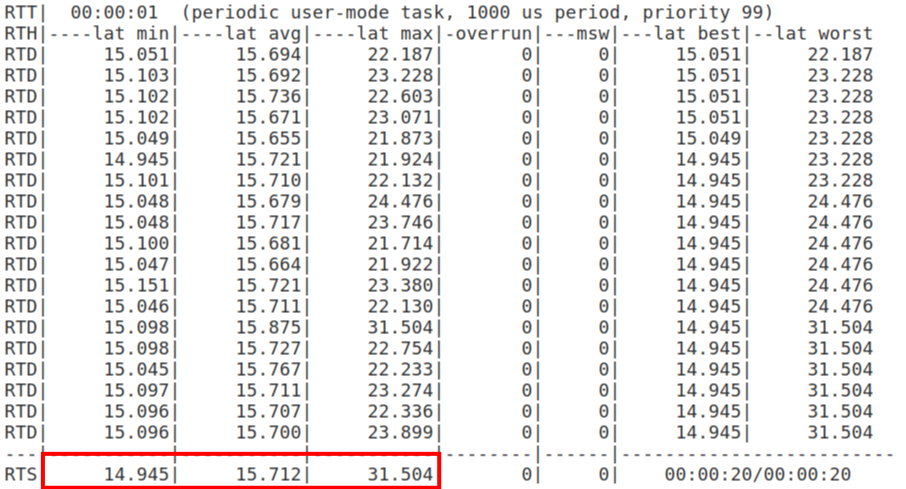
\includegraphics[width=\textwidth]{Figures/results/stat/latency_with_frame_no_sm.png}
    \caption{Latency test without running safety module.}
    \label{fig:lat_without_sm}
\end{figure}


\begin{figure}[H]
    \centering
    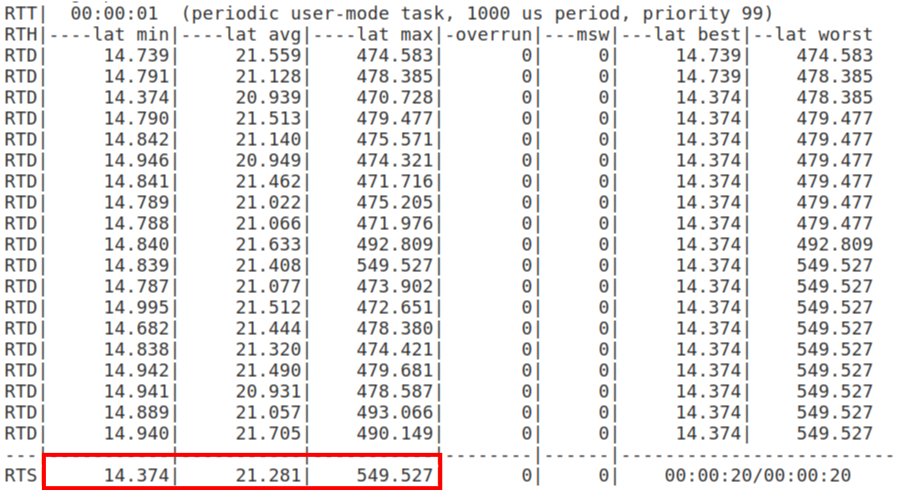
\includegraphics[width=\textwidth]{Figures/results/stat/latency_with_frame_sm.png}
    \caption{Latency test while running safety module.}
    \label{fig:lat_with_sm}
\end{figure}


% INTERPRET RESULTS IN CONCLUSION
\subsection{Mode switches and other statistics}
\label{Mode switches and other statistics}
% Talk about what how to prevent mode switching (this has already been mentioned before.)
In this section, we elaborate on the statistics of the safety module obtained with Xenomai's \texttt{stat} program. These statistics are shown in Figure \ref{fig:5sec_bad}, Figure \ref{fig:15sec_bad}, Figure \ref{fig:5sec_good} and Figure \ref{fig:15sec_good}. In all figures, the threads of interest to us, the threads of the safety module system, are highlighted with a red frame. The columns that are of interest of us the most are the \texttt{MSW} column and the \texttt{\%CPU} column. \texttt{MSW} stands for \textit{mode switch}; it denotes the number of mode switches made by a specific thread. \texttt{\%CPU} denotes the percentage of CPU used by a specific thread. Figure \ref{fig:5sec_bad} and Figure \ref{fig:15sec_bad} show the statistics of the system after watching the \texttt{stat} program using \texttt{watch} for 5 seconds and 15 seconds respectively. Figure \ref{fig:5sec_good} and Figure \ref{fig:15sec_good} show the system after watching for 5 seconds and 15 seconds as well, but after some modifications have been made to the code. We will discuss these modifications shortly, but first, let us first look at the first table of the statistics after 5 seconds shown in Figure \ref{fig:5sec_bad}.
\\\\
Notice that all of the highlighted threads are familiar to us, as we elaborated the purposes of these threads in Section \ref{Multithreaded nature of the safety module}. The only difference is that there are no \texttt{(n)rt\_retrieve\_acceleration} and \texttt{(n)rt\_retrieve\_angular\_displacement} threads, instead there are \texttt{nrt\_retrieve\_imu} and \texttt{rt\_retrieve\_imu}. This is because acceleration and angular displacement are obtained from the same IMU and they are therefore both retrieved at once.
\par
One thing that is immediately notable in the table of Figure \ref{fig:5sec_bad} is the high number of mode switches performed by the \texttt{rt\_checks} thread, which is framed in blue. If we then look at the table of Figure \ref{fig:15sec_bad}, which shows the statistics of the system after 15 seconds, we see that the number of mode switches is now roughly three times as high, which means the \texttt{rt\_checks} thread makes about 100 mode switches every 5 seconds. Recall from Section \ref{Multithreaded nature of the safety module} that the \texttt{rt\_checks} thread is the control loop originating from Dezyne that executes the five checks in sequence. Further recall from \ref{Multithreaded nature of the safety module} that real-time threads are not supposed to be making a mode switch from primary mode to secondary mode, as this transfers control over the thread from the Xenomai cokernel to the standard Linux kernel, which defeats the purpose of a real-time thread.


\begin{figure}[H]
    \centering
    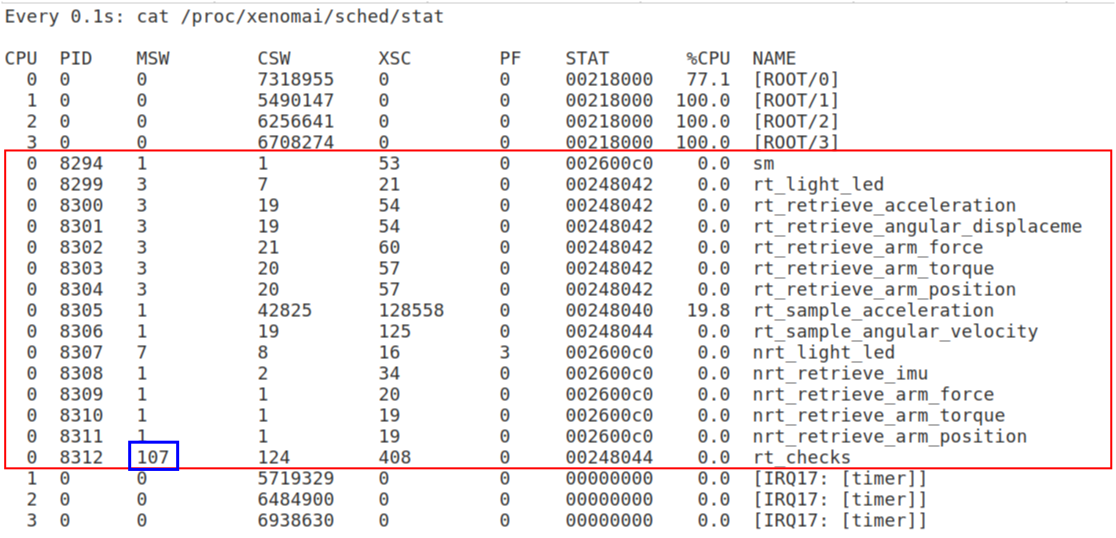
\includegraphics[width=\textwidth]{Figures/results/stat/5sec_bad_with_frames.png}
    \caption{Thread statistics (5 seconds)}
    \label{fig:5sec_bad}
\end{figure}

\begin{figure}[H]
    \centering
    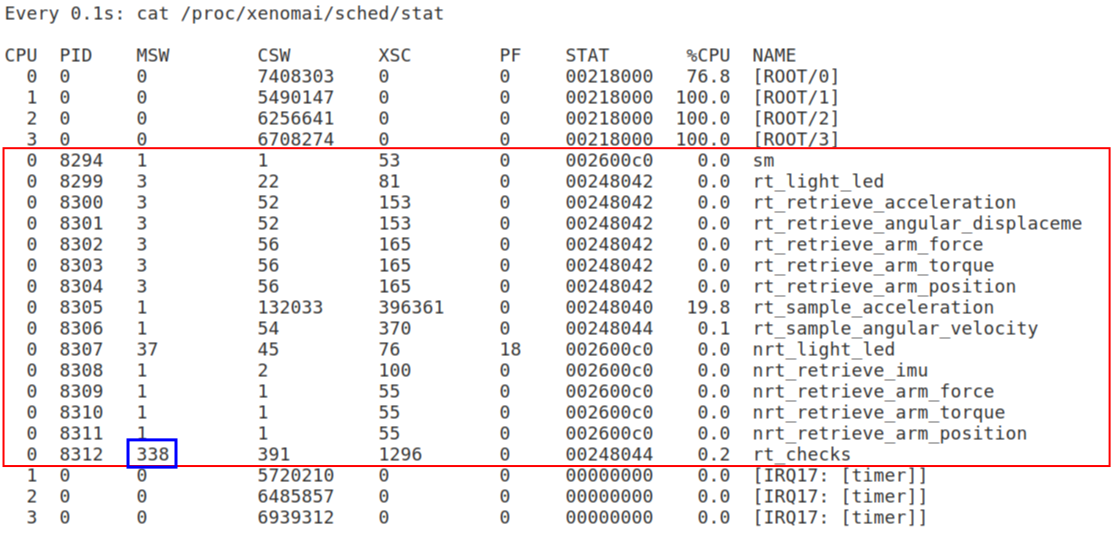
\includegraphics[width=\textwidth]{Figures/results/stat/15sec_bad_with_frames.png}
    \caption{Thread statistics (15 seconds)}
    \label{fig:15sec_bad}
\end{figure}

We figured the excessive mode switching has to do with the way Dezyne is run in the safety module, as the only operation of the \texttt{rt\_checks} thread is to execute the safety checks, of which the control logic is implemented in Dezyne. Note that, as we generate source code from the Dezyne model, in the end the Dezyne model is still just C++ code. We found that the excessive mode switching is caused by the Dezyne runtime's default behavior to print output to the output screen or to print output to a file. Since this output is not needed outside of debugging purposes, it can be disabled without a problem. This can be done by editing the source code of the Dezyne runtime directly, but we instead choose to set the output stream in our safety module code to a null stream object, which, after initialisation of the null stream object, has no operational overhead whatsoever.
\par
The table of Figure \ref{fig:5sec_good} shows the statistics after running the safety module system for five seconds after a restart of the safety module system with the excessive mode switching patch we just elaborated. In the figure we can see that the mode switching of \texttt{rt\_checks} has been reduced to just two mode switches, which is a low number as we want from a real-time thread. 

\begin{figure}[H]
    \centering
    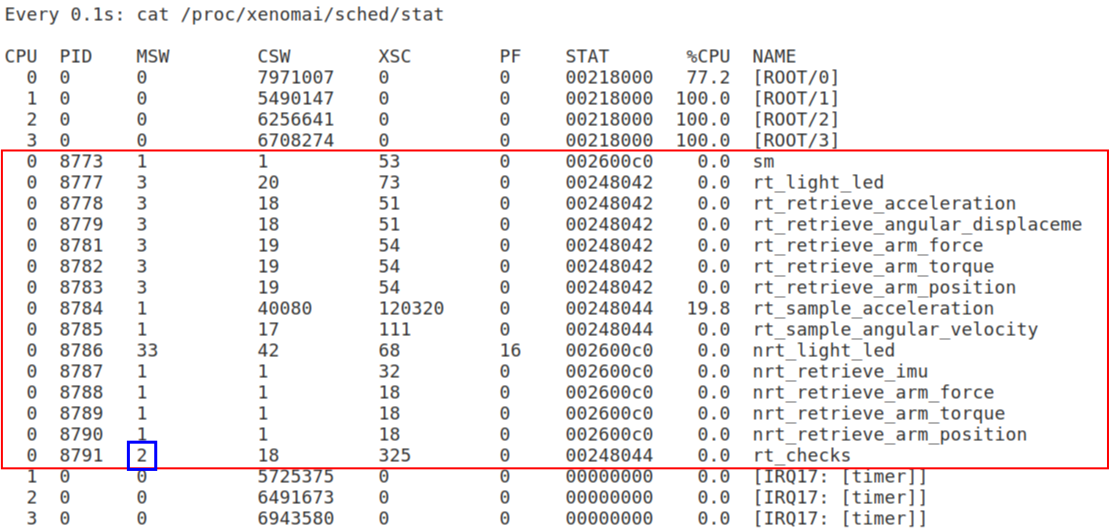
\includegraphics[width=\textwidth]{Figures/results/stat/5sec_good_with_frames.png}
    \caption{Thread statistics (5 seconds, with excessive mode switching fix)}
    \label{fig:5sec_good}
\end{figure}

For the remainder of this section, look at the table of Figure \ref{fig:15sec_good}, which shows statistics of the threads of the safety module system after running for 15 seconds and after appliance of the excessive mode switching patch. Using this table we will elaborate on some other statistics that are shown.  
\par
Let us first look at the rows of \texttt{rt\_light\_led} and \texttt{nrt\_light\_led}. Notice how\newline\texttt{rt\_light\_led} has made three mode switches and how \texttt{nrt\_light\_led} has made 55 mode switches. This is exactly what we want; the real-time thread stays in primary mode and it is the non-real-time thread that makes the switches to secondary mode to access the LED driver. Looking at the other real-time threads, we see non of them make a lot of mode switches, which is also what we want. Looking at the non-real-time threads, we see that non of these make a lot of mode switches either. This is not surprising for the \texttt{arm} threads, as they simulate interaction with ROS by just providing randomly generated sensor data. \texttt{nrt\_retrieve\_imu} on the other hand does interact with real sensors, but it need only make one mode switch.
\par
In fact, we found that all of the mode switching that is performed is performed at initialisation of the system, except in the case of the mode switching performed by \texttt{nrt\_light\_led}, which performs its mode switching throughout the entire execution of the system. This means that after initialisation of the system, \texttt{nrt\_light\_led} is the only thread that performs mode switches.
\\\\
Lastly, let us look at the \texttt{\%CPU} column shown in Figure \ref{fig:15sec_good}. We can see that, of the safety module threads, \texttt{rt\_sample\_acceleration} the highest percentage of the CPU at this timestamp (in fact, the table refreshes every $0.1$ seconds, and every $0.1$ seconds \texttt{rt\_sample\_acceleration} takes the highest percentage of CPU time. The rest of the threads take similar CPU percentages as the ones shown in this timestamp). \texttt{rt\_sample\_acceleration} has the highest CPU percentage  because of the internal calculation of velocity from acceleration that \texttt{rt\_sample\_acceleration} performs. We can see that \texttt{rt\_checks} takes a percentage of $0.4$ of the CPU and that the rest of the threads appear to be using a percentage of $0.0$ of the CPU, which has as reason that all threads except \texttt{rt\_sample\_acceleration} and \texttt{rt\_checks} have simple work to do and are rapidly done with their task. 

\begin{figure}[H]
    \centering
    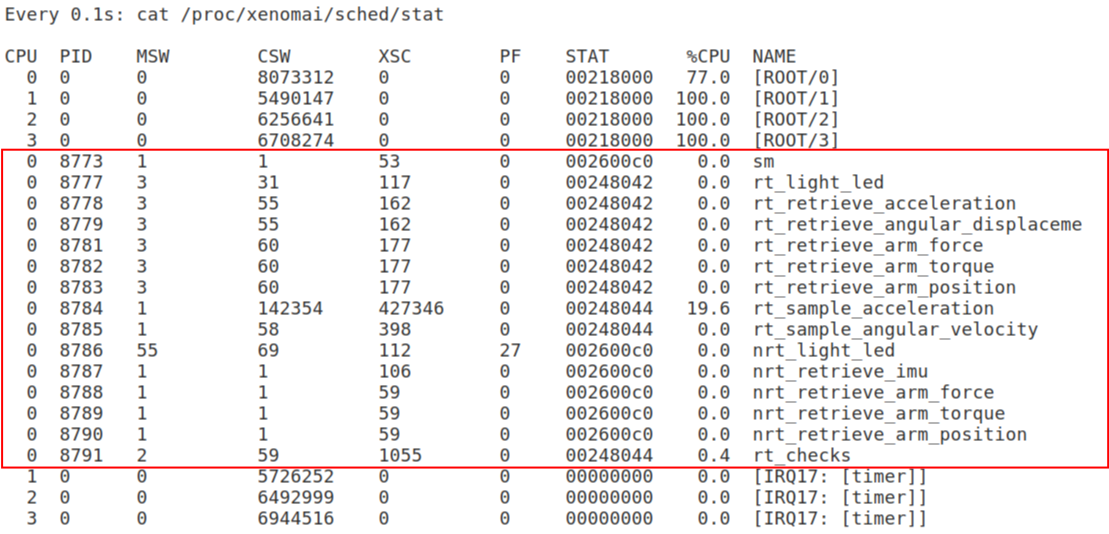
\includegraphics[width=\textwidth]{Figures/results/stat/15sec_good_with_frames.png}
    \caption{Thread statistics (15 seconds, with excessive mode switching fix)}
    \label{fig:15sec_good}
\end{figure}





\subsection{Running the safety module}
\label{Running the safety module}
In this section, we elaborate on executing the checks on the safety module. We highly recommend checking out the \href{https://github.com/Yousousen/safety-module-for-care-robot-rose}{repository}, which demonstrates the kinetic energy and rotational energy checks in video formats. These demonstrations will provide a clear view of the operation of the safety module. The kinetic energy and rotational energy demonstrations can be found in \texttt{demos} directory of the root of the repository. If checking out the repository is not an option, this section presents the kinetic energy check and rotational energy check as a series of frames. These are given in Figure \ref{fig:high_linear_acceleration} and Figure \ref{fig:high_angular_velocity} respectively.
\\\\
After initialisation the safety module will run indefinitely, running safety checks one by one. As we have elaborated in Section \ref{Multithreaded nature of the safety module}, the checks themselves are run in sequence, but the retrieval and sampling of sensor data is run continuously parallel to that. There is no requirement for how fast the checks should run, \footnote{This is not part of the assignment and requires further research. More details are in Section \ref{Refinement of timeliness of the system and scheduling} of the Recommendations}but we have set the period to be exactly the same as the poll rate of the IMU. This is to ensure sensor data is always ready to be read when a check demands it. However, since the drivers the sensor data is received from run in secondary mode, there is no guarantee that data is truly prepared when a check demands it. If the data is not prepared, the check uses the last available data. The system keeps track of the time the last data was retrieved. If the last data was retrieved too long ago the executing check will assume the behavior is unsafe, because it cannot keep track of the behavior of the care robot on time anymore. Data that is too old is set to be a time of twice the period that checks are executed, so twice the poll rate of the IMU.
\par
Let us look at two particular checks, the kinetic energy check and rotational energy check. These checks need not be simulated and can be demonstrated in real life. For both kinetic energy and rotational energy we set the limit of maximum energy to be $300$ joules. Using Equation \ref{eq:change_ke} and Equation \ref{eq:rot_energy} to solve for velocity $\vec{v}$ and angular velocity respectively, this means robot Rose can have a maximum velocity and angular velocity of $4.8$ meters per second. Note that this calculation for velocity is just that what results from a change in velocity. In other words, it does not take into account whether Rose is driving or stationary.
\par
In Figure \ref{fig:high_linear_acceleration} we can see the kinetic energy check in action. Here we started shaking the safety module slowly, and increasingly shaked it harder, so that the acceleration becomes higher. The last 12 frames of this are shown in the figure. From the fifth frame to the sixth, the velocity obtained from the acceleration causes the kinetic energy to be higher than the allowed maximum, which makes the matrix turn red to denote that this is unsafe behavior. It then takes us six more frames to stop shaking.
\par
Although this is not the case in the demonstration of Figure \ref{fig:high_linear_acceleration}, sometimes small delays are experienced between the high acceleration and the LED turning red.
\par
In Figure \ref{fig:high_angular_velocity} we can see the rotational energy check in action. This check is similar to kinetic energy, the difference being that it is concerned with angular quantities as opposed to linear quantities. In the figure we make a quick jerk from left to right, causing the rotational energy obtained from the angular velocity from frame three to frame five to be higher than the allowed maximum, thus resulting in unsafe behavior and the matrix turning red.

\begin{figure}[H]
    \centering
    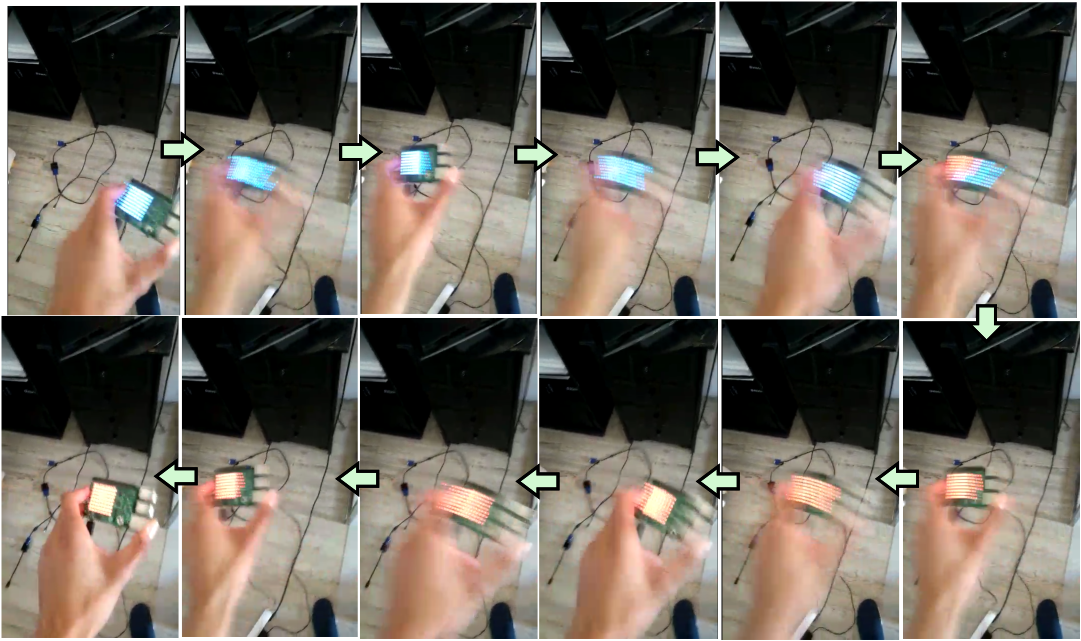
\includegraphics[width=0.9\textwidth]{Figures/results/lighting_leds/linear_acceleration.png}
    \caption{High linear acceleration will cause the matrix to turn red.}
    \label{fig:high_linear_acceleration}
\end{figure}

\begin{figure}[H]
    \centering
    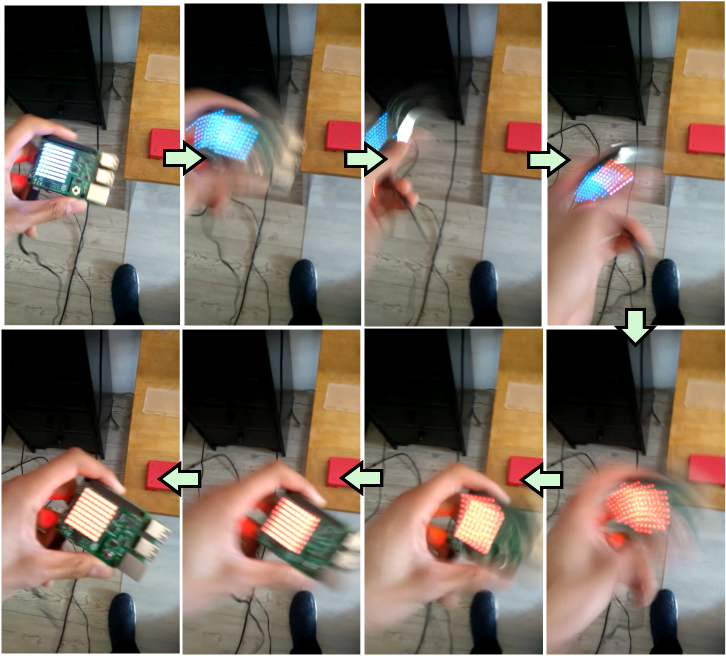
\includegraphics[width=0.6\textwidth]{Figures/results/lighting_leds/angular_velocity.png}
    \caption{High angular velocity will cause the matrix to turn red.}
    \label{fig:high_angular_velocity}
\end{figure}

The matrix cannot turn blue again until we acknowledge the unsafe behavior by clicking the reset button. Successive checks with resets in between are shown in the demonstrations on the repository.

\newpage
\chapter{Conclusion}
\label{Conclusion}
%     • herhaal onderzoeksvraag en deelvragen
% • koppel de resultaten aan de deelvragen en beantwoord de deelvragen. Let op: dit is geen herhaling van de resultaten. 
%    • in dit hoofdstuk interpreteer je de resultaten uit het vorige hoofdstuk
%    • geef antwoord op de onderzoeksvraag
%    • geen nieuwe onderwerpen/feiten in de conclusie

% Start with the word 'feasibility study'.
In this research, we conducted a feasibility study to determine the feasibility of combining ideas from the fields of mobile robotic safety, verification of system behavior and real-time systems, and applying the combination of these ideas to a safety module for care robot Rose. To determine the feasibility we asked ourselves how a real-time safety module can be designed and implemented that provides an extra layer of safety in order to prevent injury to patients or damage to the environment because of collision, clamping or pinching caused by care robot Rose. This principal research question was worked out into four subsquestions, from which the results were given Section \ref{Choice of hardware and software}, Section \ref{Retrieving and Using Sensor Data}, Section \ref{Formal model of the behavior of the system} and Section \ref{Implementation} of the Results. We will now interpret the results of these subquestions.

\section{Conclusion on the hardware and the operating system}
In Section \ref{Choice of hardware and software} the results of our literature study and comparative study were given. There we found that the \gls{pi} with Sense HAT is the best hardware platform according to the requirements specified. We think the \gls{pi} with the Sense HAT is an excellent choice in terms of scalability and further versions of the safety module. We elaborated how the built in \gls{wifi} card can be used to communicate with Rose and her operator, and how additional sensors on the Sense HAT can be used to obtain more data from the environment.
\par
In the comparative study, we compared different hardware platforms, but we did not go in depth about different versions of the hardware platform. For example, in the case of the \gls{pi}, a comparison could be made between the \gls{pi} Zero W, the \gls{pi} 3 and the \gls{pi} 4. The comparison of different versions of the hardware platform is given in Section \ref{pi versions and costs}  of the Recommendations.
\par
In Section \ref{Choice of hardware and software}, we elaborated how the Xenomai framework has better real-time performance for our purposes than the Real-time Linux patches to the standard Linux kernel. In Section \ref{tOS} we saw that the Xenomai framework is able to provide hard real-time performance in kernelspace. Thus, using the Xenomai framework for the prototype safety module provides a solid ground for further versions of the safety module, in which we may want to port the userspace system to kernelspace. The use of the POSIX skin and XDDP sockets is also scalable; because of the POSIX skin and XDDP sockets new sensors (including sensors from robot Rose through ROS) can be added to the safety module without the need to port their drivers to the Xenomai-framework.

\section{Conclusion on the usage of sensor data and the detection of unsafe behavior}
In Section \ref{Retrieving and Using Sensor Data}, we elaborated our findings on how to retrieve sensor data and on how to use it to check for unsafe behavior. There we found that the IMU of the Sense HAT can be used to retrieve acceleration and angular velocity. This is useful, because this provides us with a way to measure the kinetic energy and rotational energy independently from robot Rose. Values for the time intervals $\Delta t$ were determined experimentally and set to be a multiple of the IMU poll rate to provide a common multiple of time throughout the system, but we do not think this is an optimal time interval. In fact, setting the $\Delta t$'s to this value may be the cause of the small delays that sometimes occur as mentioned in Section \ref{Running the safety module}. But since our research's objective is to show the feasibility of the safety module instead of mainly focusing on the timeliness of the system, we did not aim for the most optimal time intervals.
\par
Regardless of the timing, the equations prove to work well to detect unsafe behavior, as has been shown in the demonstrations in Section \ref{Running the safety module}. 


\section{Conclusion on the modelling of the safety module's behavior}
\label{On modelling safety module behavior}
In Section \ref{Formal model of the behavior of the system}, we modelled the behavior of the safety module. The model puts some guarantees on the behavior of the safety module; like the affirmation that there are no deadlocks and livelocks. This affirmation is not limited to the model but propagated to the implementation code as well, because the source code that is generated from the Dezyne models is bound and called from the implementation code. As we aimed for the hardware platform of the safety module to be extensible and scalable for future additions, we also made sure the model can be easily augmented with new safety checks, by implementing the checks as elements of a linked list. The only downside that comes with this abstraction of checks to elements of a linked list is that the sequence diagrams of the controller no longer show what checks are being executed. This is merely a drawback in the generation of the sequence diagrams; in the implementation code all information about individual checks is still available.

\section{On the implementation of the safety module}
\label{On the implementation of the safety module}
% Note achieving soft real-time performance
In Section \ref{Implementation}, we elaborated how we implemented the model of the safety module on the operating system with the Xenomai framework and we elaborated its interaction with the other threads in the system. In Section \ref{Implementation}, Figure \ref{fig:lat_without_sm} and Figure \ref{fig:lat_with_sm} showed the latency of the system without running the safety module program and the latency while running the safety module program respectively. We noticed the increase in the maximum latency when running the safety module program. The increase in maximum latency is not a problem, for we have no requirement on what the maximum latency of the system should be. Still, the Figure \ref{fig:lat_with_sm} shows that if the system is put under sufficiently large load the response time to a given stimuli decreases. We also noted that the minimum latency and average latency under load of the safety module program does not differ very much from the minimum latency and average latency when the safety module is not running. The average latency is closer to the the minimum latency in both cases, which means we only reach the maximum latency seldom or it means our executed period test tasks resemble a bimodal distribution skewed to the left. Looking at the \texttt{lat min} and \texttt{lat avg} columns of Figure \ref{fig:lat_with_sm} we can exclude the latter because we see that \texttt{lat avg} data is simply just close to the \texttt{lat min} data. So we can conclude that maximum latency appears seldom. A few cases of maximum latency is not a problem if we see the safety module as a soft real-time system. \footnote{In Section \ref{Assignment specification} we explained why we aim for a soft real-time system and not a hard real-time system.}
\par
But we have not yet concluded that the safety module achieves soft real-time operation. That the safety module achieves soft real-time operation follows from the last statistics table of Section \ref{Implementation}, given in Figure \ref{fig:15sec_good}. To explain, in Section \ref{Operating System}, we elaborated how the Xenomai framework achieves real-time operation. In Section \ref{tOS} we saw that Xenomai userspace programs can achieve soft real-time operation at most. The conclusion that can be drawn from these sections is that soft real-time operation of the safety module is achieved by keeping the real-time threads of the safety module running in primary mode. We said that real-time threads should not leave primary mode, for if they would they would not be real-time threads. We defined real-time threads to be threads that do not leave primary mode, and this conforms to what Xenomai thinks of as a real-time thread. We noted at the end of Section \ref{Implementation} that the only time any of the \texttt{rt} threads makes a mode switch to secondary mode, it is at initialisation of the safety module. After initialisation, none of the \texttt{rt} threads will make a mode switch to secondary mode. This can be seen by comparing the table in Figure \ref{fig:15sec_good} to the table in the preceding figure, Figure \ref{fig:5sec_good}. The difference in time between these figures is ten seconds and in those ten seconds non of the real-time threads have made additional mode switches.\footnote{To truly confirm no additional mode switches are made by the real-time threads we ran it for a couple of minutes and simulated some unsafe behavior. As expected, the mode switch count of any of the real-time threads did not increment.} Because non of the real-time threads make additional mode switches after initialisation, we can conclude that the safety module achieves soft real-time operation.

\section{Discussion on the final result}
% At the end, conclude that it is feasible and why
Looking at the running safety module shown in Section \ref{Running the safety module} of the Results, we think our aim of designing and implementing a safety module that provides an extra layer of safety with the goal to prevent injury to patients or damage to the environment because of unsafe behavior has been achieved. Aside from some minor delays in turning the matrix red that happen every now and then, the safety module works as expected. Moreover, since we achieved soft real-time operation of the safety module, we think we have also affirmed the feasibility of this setup of the system as a whole.

\newpage
\chapter{Recommendations}
\label{Recommendation}
%     • afhankelijk van het onderzoek is dit een apart hoofdstuk. 
    % • goede aanbevelingen zijn helder, voor 1 uitleg vatbaar en resultaatgericht.
    % • de aanbevelingen zijn haalbare suggesties die op redelijk korte termijn te realiseren zijn. Geen vage opmerkingen die in een onbekende toekomst misschien van toepassing zijn.
    % • verwijs bij de aanbevelingen altijd terug naar de eerder gedane bevinden.
    
In this section we present our recommendations for further research on the safety module. Most of the recommendations are refinements of the base system that was laid out in this research.

\subsection{Testing the safety module on care robot Rose}
In this research we did not test the prototype safety module on care robot Rose. The prototype safety module makes use of the sensors of its own hardware platform, the sensors on the Sense HAT,to retrieve data from the environment. Although ROS is installed on the safety module, functions that are to interact with ROS are implemented as stubs. Therefore, the first and foremost recommendation for further research is to create the interface from the safety module to ROS and to test the safety module on care robot Rose.

\subsection{\gls{pi} versions and costs}
\label{pi versions and costs}
In Section \ref{Choice of hardware and software}, we found that the \gls{pi} was the best hardware platform to work with, but our research did not go in depth about different versions of the \gls{pi}. We recommend further research to compare different versions of the \gls{pi}, like the \gls{pi} Zero W, the \gls{pi} 3 (used in this research) and the \gls{pi} 4, in terms of performance and costs. For instance, it could be that there is significant performance to be gained by use of the more expensive \gls{pi} 4 over the \gls{pi} 3, but this may not be worth it economically. Likewise, the cheaper \gls{pi} Zero W may be considered, but it may not have the required hardware capabilities.

\subsection{Conversion to Xenomai kernel space for hard real-time performance}
In the literature review of Section \ref{tOS}, we found that in order to achieve hard real-time performance, the safety module system should be implemented in Xenomai kernelspace. In this research, soft real-time performance is achieved by use of Xenomai userspace tasks. A reasonable step for follow-up research would be to port the existing Xenomai userspace system of this research to Xenomai kernelspace.

\subsection{Refinement of safety metrics}
\label{Refinement of safety metrics}
In this research, we use a rudimentary form of the safety metrics presented in the literature review of Section \ref{Safety in care robots}. To increase the efficacy of the safety module, we recommend follow-up research to refine these safety metrics.

\subsection{Refinement of timeliness of the system}
\label{Refinement of timeliness of the system and scheduling}
In this research, the periods of threads and time intervals used in calculations (like the $\Delta t$'s used in the numerical integration and the numerical differentiation) were determined experimentally and set to be a multiple of the IMU poll rate, but this is not necessarily the most optimal timing. Follow-up research could conduct a study to determine what the most optimal timing for the system is in terms of periods of threads, sample time and time intervals in calculations.

\subsection{Addition of time verification in the behavioral model}
\label{Addition of time verification in the behavioral model}
In our research, the behavioral module created with Dezyne does not take into account how much time it takes to execute certain actions. In addition to the recommendation to refine the timeliness of the system elaborated in Section \ref{Refinement of timeliness of the system and scheduling}, we recommend to verify the timeliness in the behavioral model.



%\section{Discussion} \label{Discussion}
%% • evalueer het onderzoek en het product
%% • voorstel voor vervolgonderzoek

%%% APPENDICES %%% 
\begin{appendices}

\chapter{Short introduction to the Dezyne toolset}
\label{Short introduction to the Dezyne toolset}
In this appendix, we present a short overview of the Dezyne toolset that is used in this research to model behavior of the safety module. We think it is important to show a simple example to get across the effectiveness of the toolset and the relevance of the toolset in our research. 

\subsection{The Dezyne modelling language}
\label{The Dezyne toolset and the Dezyne modelling language}
We will now look at the basics of the Dezyne modelling language and verification mechanisms. For this we will construct a short model that turns a LED on, off or lets it blink. Inspiration for this model has been taken from the Dezyne documentation (\cite{dzntut}). The model is shown in Listing \ref{fig:theoretical_background_dezyne_model}.

\begin{listing}[!ht]
\begin{minted}[mathescape,
               numbersep=5pt,
               frame=lines,
               framesep=5mm,
               linenos]{haskell}
               
interface ILED {
    enum State { Off, On };
    in void turnOn();
    in void turnOff();
    in State getState();

    behaviour {
        State state = State.Off;

        [state.Off] {
            on turnOn: { state = State.On; }
            on turnOff: { state = State.Off; }
            on getState: { reply(state); }
        }
        [state.On] {
            on turnOn: { state = State.On; }
            on turnOff: { state = State.Off; }
            on getState: { reply(state); }
        }
    }
}

component LED {
    provides ILED iLed;

    behaviour {
        ILED.State state = ILED.State.Off;

        [state.Off] {
            on iLed.turnOn(): state = ILED.State.On;
            on iLed.getState(): reply(state);
        }
        [state.On] {
            on iLed.turnOff(): state = ILED.State.Off;
            on iLed.getState(): reply(state);
        }
    }
}

\end{minted}
\caption{Dezyne model that turns a LED on and off}
\label{fig:theoretical_background_dezyne_model}
\end{listing}

%\begin{figure}[H]
%    \centering
%    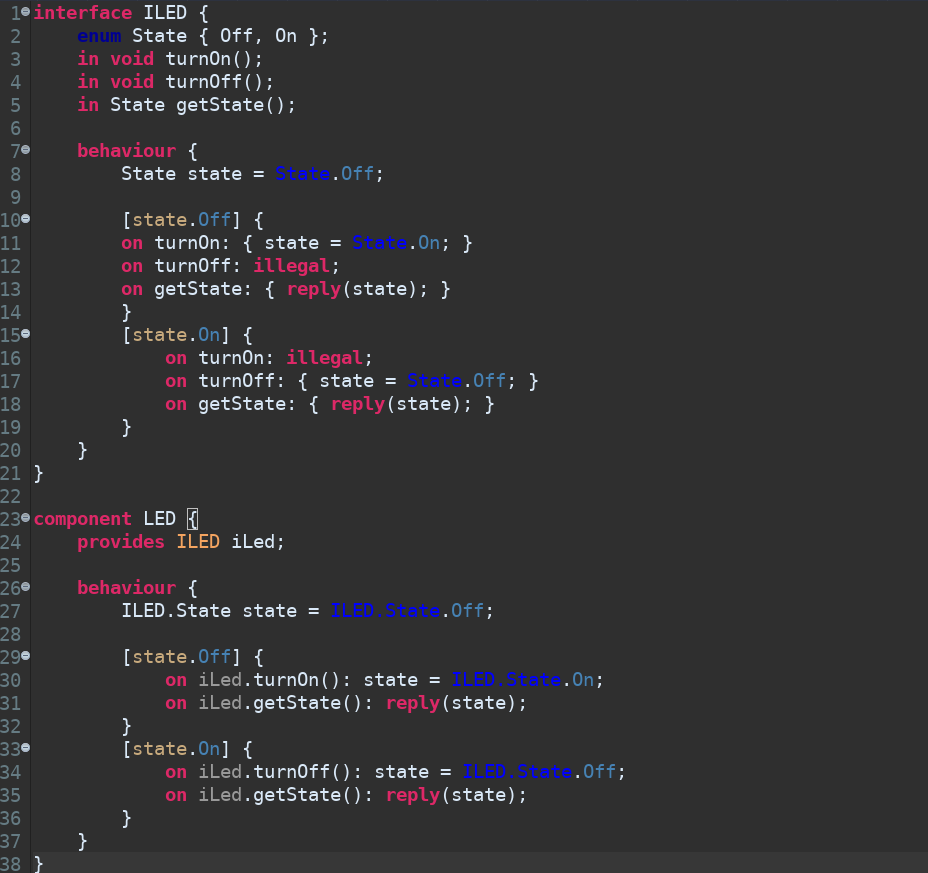
\includegraphics[width=\textwidth]{Figures/theoretical_background/enhanced_diagram.png}
%\end{figure}

First of all, notice the notions of an \textit{interface} and a \textit{component} from Lines 1 to 21 and 23 to 38 respectively. Dezyne breaks logical control problems into components and interfaces. An interface defines the following: how a component interacts, the events that can be communicated and the interaction protocol (\cite{dzndoc}). In other words, it defines the behavior of a component, the events that it can execute and in what states it can execute those events. In Line 2 we can see an enum declaration. This enum defines the states the system can be in. Below that, in Lines 3 to 5 we see the event declarations of the system. %Events are implemented as function calls in code (\cite{dzngloss}), as we will see in Section \ref{Generating code from a verified Dezyne model}.
From Line 7 to 20 we see the \textit{behaviour} block of the interface. Here we define in what states certain events are allowed, or what events should bring the system into a certain state. In this example, we have chosen to declare behavior state-first, meaning we specify the state of the system first and then we specify which actions can occur in that state, but the language allows for behavior to be declared event-first as well, in which we would specify the event first and then specify the states.
% Continue with turnOn turnOff getState, illegal, then component
In Line 8 we declare that the system starts off in the \texttt{State.Off} state. Then, in Line 10 to Line 14, we specify that when the system is in the \texttt{State.Off} state, we allow the \texttt{turnOn} and \texttt{getState} events to fire, but that \texttt{turnOff} is \texttt{illegal}, which as the keyword suggests makes the event illegal to fire. This makes sense, as when we are already in the \texttt{State.Off} state we cannot turn the system off. The \texttt{turnOn} event sets the state to \texttt{State.On}, and the \texttt{getState} event, using the \texttt{reply} keyword, returns the current state of the system when the event fires. In Lines 15 to 19 we specify what should happen when the system is in the \texttt{State.On} state. When the system is in the \texttt{State.On} state, the \texttt{turnOn} state firing should be illegal, as we cannot turn the system on when it is already on. The \texttt{turnOff} state turns off the system by setting the state to \texttt{State.Off}, and the \texttt{getState} event returns the current state of the event, just like when the system is in the \texttt{State.Off} state.
\\\\
We will now look at the component declared in Lines 23 to 38. A component is a unit of definition and instantiation (\cite{dzngloss}). A component defines zero or more \textit{ports}, where a port is a named instance of an interface (\cite{dzngloss}). \texttt{provides} is the keyword used to define a port. In our example, the defined port is \texttt{iLed}, an instance of the interface \texttt{ILED}. The idea of the behavior of a component is that it conforms to the behavior of its specification, or interface. We therefore make it start in the same state as the interface does in Line 27. In Line 29 to Line 36 we specify the behavior of the component. Notice how, in this example, the behavior is the same, except that the events that are illegal are not specified. These need not be specified because the component infers what is illegal behavior from its provided interface. This is because verification of a component always goes through its interface, as we will see in Section \ref{Verifying a Dezyne model}. In this example the component's behavior block is almost exactly the same as the interface's behavior block. This is because the example is simple, more complex models will show more differences between the behavior blocks of the component of the interface. Nonetheless, the behavior of the component should always conform to the behavior of the interface.
\\\\
Figure \ref{fig:led_example_graph} shows the state chart of our example LED model.

\begin{figure}[H]
    \centering
    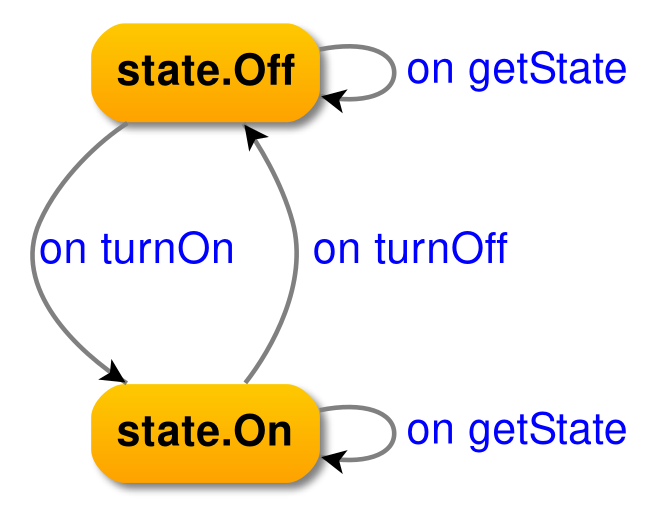
\includegraphics[width=0.5\textwidth]{Figures/theoretical_background/led_example_graph.png}
    \caption{State chart for the LED model}
    \label{fig:led_example_graph}
\end{figure}

In Figure \ref{fig:led_example_graph} we can see the \texttt{State.Off} and \texttt{State.On} states and  the \texttt{turnOn}, \texttt{turnOff} and \texttt{getState} events we declared in code of the model in Figure \ref{fig:theoretical_background_dezyne_model}.

\subsection{Verifying a Dezyne model}
\label{Verifying a Dezyne model}
We will now look at the verification features of the Dezyne toolset. We will look at these features in context of the model in Listing \ref{fig:theoretical_background_dezyne_model}. Let us first verify the interface. When we verify the interface as it is given in Listing \ref{fig:theoretical_background_dezyne_model}, we get the message back that there are no verification errors in the interface. But things are not always so straightforward. Suppose that we forget to specify the \texttt{getState} event on Line 13. If we then verify the model we will get the error message shown in Figure \ref{fig:not_specifying_all_events_error}.

\begin{figure}[H]
    \centering
    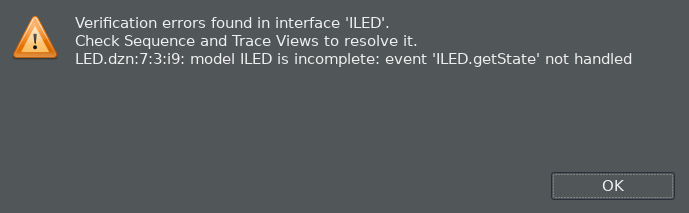
\includegraphics[width=0.7\textwidth]{Figures/theoretical_background/verification_of_interface_error.png}
    \caption{Interface verification error: Not specifying all events}
    \label{fig:not_specifying_all_events_error}
\end{figure}

The reason we get this verification error is that a well defined interface should specify the behavior of any of its declared events, and that behavior should be specified for every state of the system. When we do not declare the \texttt{getState} event on Line 13, we have not specified what behavior should take place if the \texttt{getState} event fires while the system is in the \texttt{State.Off} state.
\\\\
Let us return to the correct code as given in Listing \ref{fig:theoretical_background_dezyne_model} and let us now verify the component. The code of the component as it has been given in Listing \ref{fig:theoretical_background_dezyne_model} shows no first verification errors. In case a component gets through verification without errors we see a table like the one shown in Figure \ref{fig:Table showing no verifcation errors in the LED component}.

\begin{figure}
    \centering
    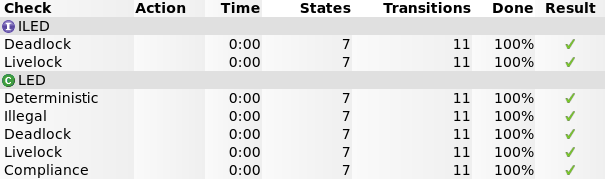
\includegraphics[width=0.8\textwidth]{Figures/theoretical_background/led_verification.png}
    \caption{Table showing no verification errors in the LED component}
    \label{fig:Table showing no verifcation errors in the LED component}
\end{figure}

In Section \ref{The Dezyne toolset and the Dezyne modelling language}, we noted how verification of a component is always in context of its interface. We can see this fact in Figure \ref{fig:Table showing no verifcation errors in the LED component}, as interface \texttt{ILED} is first checked for deadlocks and livelocks before we check the \texttt{LED} component. The \texttt{ILED} interface shows no errors so the verifier goes on to the LED component. We can see that the component is checked for determinism, illegal statements, deadlocks, livelocks and compliance. Determinism in computer science refers to deterministic behavior of an algorithm. In Dezyne determinism means that for every state there is a unique implementation for every event. There cannot be multiple definitions of a particular state in a event.
% A deterministic algorithm is expected to produce the same output no matter what its input is (\cite{determinism}).
The illegal statements refer to whether the component tries to execute an event that is deemed illegal by its provided interface. The definitions of deadlock and livelocks we have given in Section \ref{Terms and defintions}. Compliance refers to whether the component conforms to the behavior as specified in the interface.
\par
Let us now look at an instance of verification of a component where we get errors in the verification. Suppose we add the line: '\mintinline{c}{on iLed.turnOff(): state = ILED.State.Off;}' above Line 30 in the code of Listing \ref{fig:theoretical_background_dezyne_model} to try and turn the LED off while it is in the off state. Since the interface the component provides does not specify that the \texttt{iLed.turnOff()} event can fire in the \texttt{State.Off} state, we get an error showing that the \texttt{iLed.turnOff()} event is not allowed by port iLed, as shown in Figure \ref{Component verification error: Not confirming to the interface}. Additionally, Dezyne shows a sequence diagram of a trace that leads to the error, as shown in Figure \ref{Sequence diagram showing that the component does not conform to the interface}. In this case, the trace is very short as the first event that executes, namely \texttt{turnOff}, is the cause of the problem.

\begin{figure}[H]
    \centering
    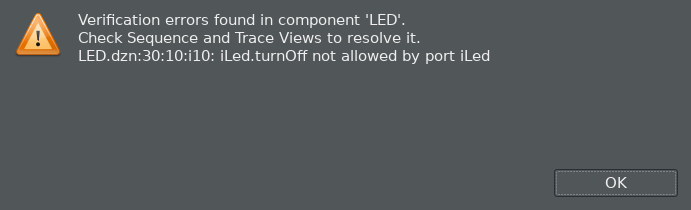
\includegraphics[width=0.7\textwidth]{Figures/theoretical_background/led_verification_error.png}
    \caption{Component verification error: Not confirming to the interface}
    \label{Component verification error: Not confirming to the interface}
\end{figure}

\begin{figure}[H]
    \centering
    
\includegraphics[width=\textwidth]{Figures/theoretical_background/verification_error_in_sequence_diagram.png}
    \caption{Sequence diagram showing that the component does not conform to the interface}
    \label{Sequence diagram showing that the component does not conform to the interface}
\end{figure}

From this we can see that the interface prevents us from executing actions (events) that are not allowed by it. Let us remove the \texttt{turnOff} action, so that we end up with the code in Listing \ref{fig:theoretical_background_dezyne_model} again. Suppose we removed Line 35: \texttt{on iLed.getState(): reply(state)}. If we then verify the model, we get an error saying that getState is an implicitly illegal action, as we can see in Figure \ref{Component verification error: getState implicitly illegal}. The accompanying sequence diagram is shown in Figure \ref{Sequence diagram showing that getState is an illegal action in the component}.

\begin{figure}[H]
    \centering
    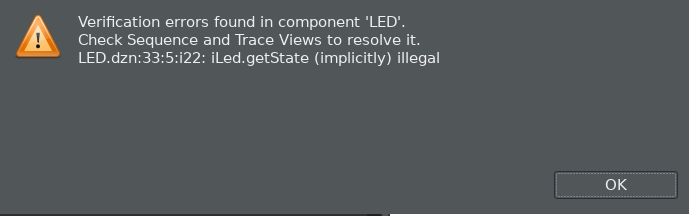
\includegraphics[width=0.7\textwidth]{Figures/theoretical_background/led_verfication_error_getState.png}
    \caption{Component verification error: getState implicitly illegal}
    \label{Component verification error: getState implicitly illegal}
\end{figure}

\begin{figure}[H]
    \centering
    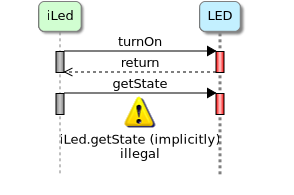
\includegraphics[width=0.5\textwidth]{Figures/theoretical_background/getState_implicitly_illegal.png}
    \caption{Sequence diagram showing that getState is an illegal action in the component}
    \label{Sequence diagram showing that getState is an illegal action in the component}
\end{figure}

The reason we get the error shown in Figure \ref{Component verification error: getState implicitly illegal} and Figure \ref{Sequence diagram showing that getState is an illegal action in the component} after removing Line 35 is because not specifying an event means that the event is illegal in Dezyne. But this is in contrast to what we specified in the \texttt{ILED} interface. We did not specify that \texttt{getState} is illegal in the interface, therefore the error states that \texttt{getState} is \textit{implicitly} illegal.
\par
The lesson learned from this example is that a component must always conform to what is specified in its provided interface.
\\\\
Lastly, let us look at a sequence diagram for the correctly verified model of Listing \ref{fig:theoretical_background_dezyne_model}. The sequence diagram is shown in Figure \ref{Sequence diagram of the LED component}. This is also called a simulation in Dezyne, because we simulate the system's control logic, taking a particular walk through the available actions. In this research, when we refer to a component's actions, we mean the same thing as the events we have declared for it. At the bottom of Figure \ref{Sequence diagram of the LED component} we can see the particular actions we can execute, that is, events that can fire in this system's state, and on the right we see a watch window that shows values of the variables of the interface and the component. Since this example consists of just a \texttt{LED} component and its interface, the sequence diagram does not give us much information that we could not already deduce from the state diagram in Listing \ref{fig:led_example_graph}. However, for more complex systems like our safety module given in Section \ref{Formal model of the behavior of the system}, the sequence diagrams will prove to be a very useful visualisation of the system.
\\\\
In Section \ref{Generating code from a verified Dezyne model} we will look at the C++ code we can generate from our LED example model.

\begin{figure}[H]
    \centering
    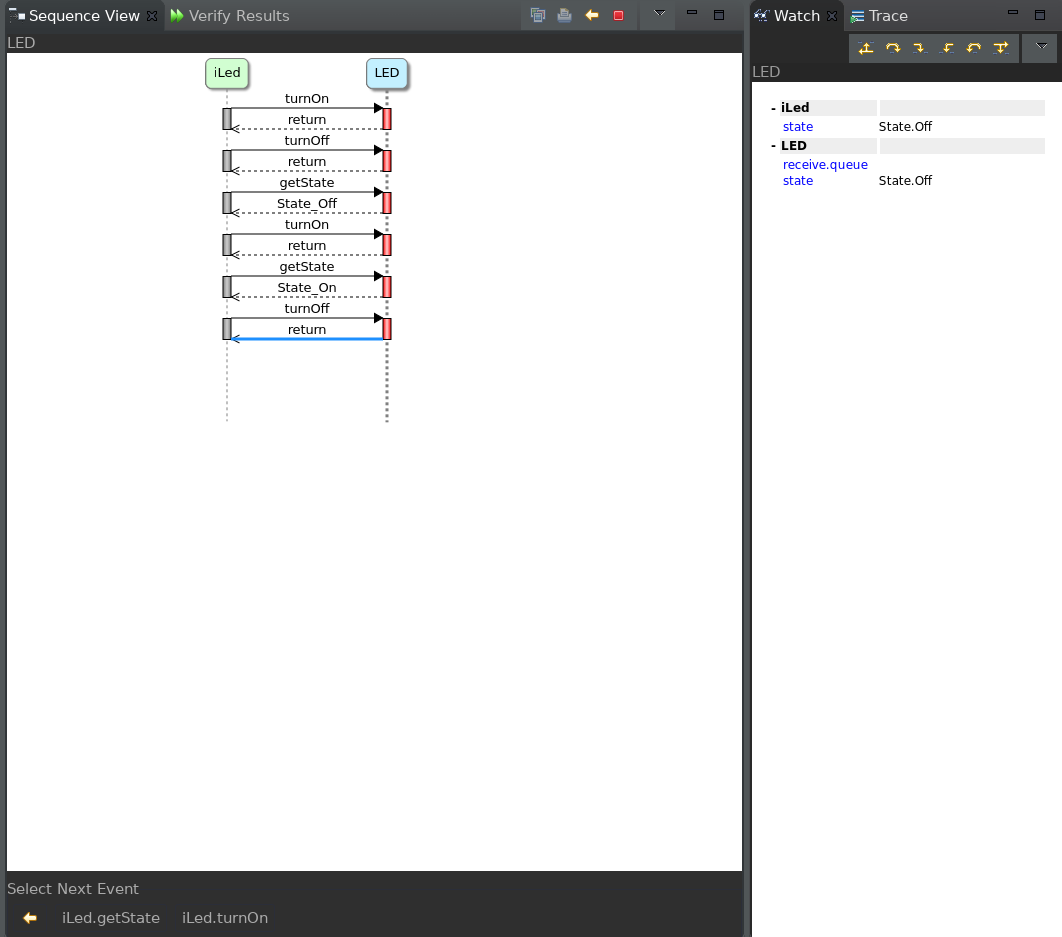
\includegraphics[width=\textwidth]{Figures/theoretical_background/simulation_of_led.png}
    \caption{Sequence diagram of the LED component}
    \label{Sequence diagram of the LED component}
\end{figure}


\subsection{Generating code from a verified Dezyne model}
\label{Generating code from a verified Dezyne model}
In this section, we will look at the code generation feature of Dezyne. We will make use of the model from Listing \ref{fig:theoretical_background_dezyne_model} for the generation of the code. To make the demonstration simpler, instead of letting the \texttt{turnOff} and \texttt{turnOn} events be illegal on Lines 12 and 16, we simply switch the state to \texttt{State.Off} and \texttt{State.On} respectively. We also added those actions to the component. Furthermore, to demonstrate the system component, which will be useful in code generation, we added a \texttt{IController} interface, a \texttt{Controller} component and a system component above the \texttt{ILED} interface. These additions are shown in Listing \ref{Addition of interface IController, component Controller and system component}. The system component generates a System view, which is shown in Figure \ref{System view of the controller and led system}.
    
\begin{listing}[!ht]
\begin{minted}[mathescape,
               numbersep=5pt,
               frame=lines,
               framesep=5mm,
               linenos]{haskell}
               
component System {
	provides IController iController;
	system {
		Controller controller;
		LED led;
		iController <=> controller.iController;
		controller.iLed <=> led.iLed;
	}
}

interface IController {
	in void trigger();
	in void stop();
	behaviour {
		on trigger: {}
		on stop: {}
	}
}

component Controller {
	provides IController iController;
	requires ILED iLed;
	behaviour {
		on iController.trigger(): iLed.turnOn();
		on iController.stop(): iLed.turnOff();
	}
}

\end{minted}
\caption{Addition of interface IController, component Controller and system component}
\label{Addition of interface IController, component Controller and system component}
\end{listing}
               
%\begin{figure}[H]
%    \centering
%    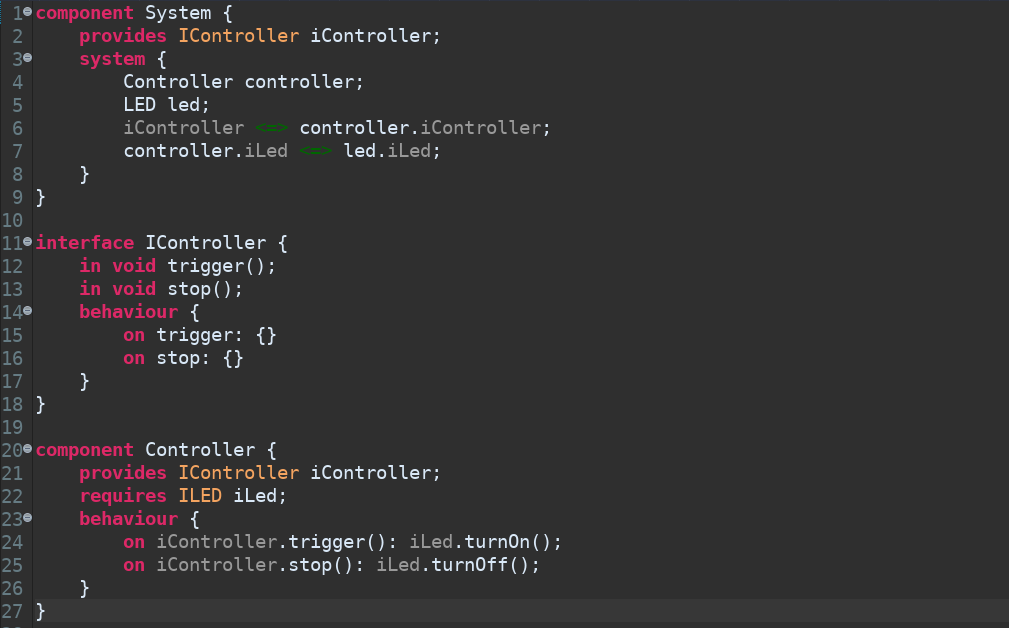
\includegraphics[width=\textwidth]{Figures/theoretical_background/system_component.png}
%    \caption{Addition of interface IController, component Controller and system component}
%    \label{Addition of interface IController, component Controller and system component}
%\end{figure}

\begin{figure}[H]
    \centering
    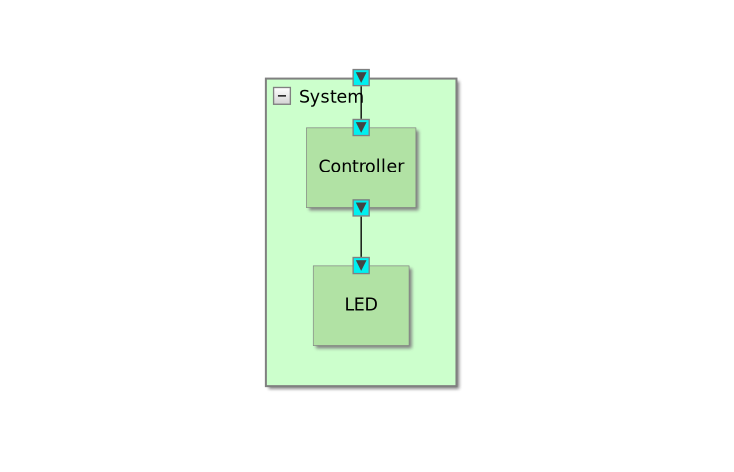
\includegraphics[width=0.9\textwidth]{Figures/theoretical_background/sys_view.png}
    \caption{System view of the controller and LED system}
    \label{System view of the controller and led system}
\end{figure}

The Controller's job is to simply turn the LED on and off with its \texttt{trigger} and \texttt{stop} functions. We can see that it does that by calling the \texttt{iLed.turnOn} and \texttt{iLed.turnOff} events. In Line 22 of Listing \ref{Addition of interface IController, component Controller and system component} we specified that the controller component will call events from \texttt{ILED} with the \texttt{requires} keyword. In the component called \texttt{System} we see some more new syntax.  The system section, as indicated by the keyword \texttt{system}, consists of two parts: instantiations of subcomponents, followed by all the bindings among the sub-components and ports of the component. This results in the system view shown in  Figure \ref{System view of the controller and led system}. This system view shows all the components of the system. We will see how the system view is useful to us in the generated code shortly.
\\\\
We will now generate source code from the model. Dezyne provides the option to generate code in a variety of languages. For this example we choose to generate C++ code, as C++ is the language used for the safety module as well. In Listing \ref{lst:led_example code} we show a very minimal main function to use the generated code and Figure \ref{Execution of minimal led example code} shows the execution of the compilation of this code. The generated code itself can be found on \href{https://github.com/Yousousen/safety-module-for-care-robot-rose.git}{our github repository}.

\begin{listing}[ht]
\begin{minted}[mathescape,
               numbersep=5pt,
               frame=lines,
               framesep=5mm,
               linenos]{c}
               
#include <iostream>
#include <dzn/runtime.hh>
#include <dzn/locator.hh>
#include "LED_example.hh"

int main() {
    dzn::locator loc;
    dzn::runtime rt;
    loc.set(rt);
    System s(loc);
    s.dzn_meta.name = "LedExampleSystem";
    s.check_bindings();

    std::string input;
    while(1) {
        std::cin >> input;
        if (input == "On")
            s.iController.in.trigger();
        else if (input == "Off")
            s.iController.in.stop();
    }
    return 0;
}

\end{minted}
\caption{Example source code}
\label{lst:led_example code}
\end{listing}

\begin{figure}[H]
    \centering
    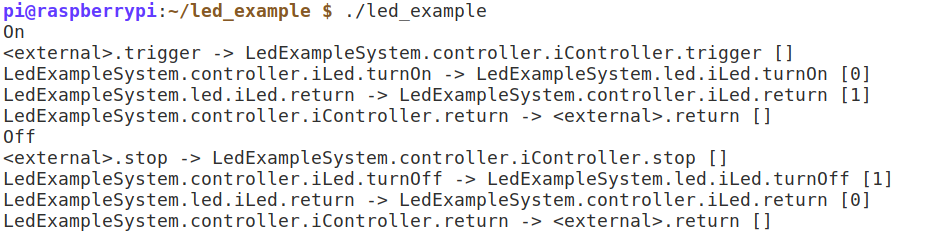
\includegraphics[width=\textwidth]{Figures/theoretical_background/executed.png}
    \caption{Execution of minimal LED example code}
    \label{Execution of minimal led example code}
\end{figure}

Lines 7 to 11 have to do with the allocation and use of the Dezyne runtime. Usage of the Dezyne runtime is elaborated extensively in the documentation of the toolset (\cite{dzndoc}). On Line 10 we declare a system object. The system object is useful because we can use it to check whether every function from dezyne is bound to a function in our C++ code and we can access our dezyne functions, \texttt{trigger} and \texttt{stop} through it, as is done on Line 18 and Line 20 respectively. In our simple example we have not bound any Dezyne functions to C++ code. In a real system we would bind the LED's \texttt{turnOn} and \texttt{turnOff} events to C++ functions that are able to turn a real LED on and off. Examples of the binding of Dezyne events to functions can be found in the Dezyne documentation or in our Results on the implementation of the safety module in Section \ref{Binding Dezyne events to functions}. 
\par
The executed code in Figure \ref{Execution of minimal led example code} shows how we simulate turning on and off a LED by giving the program the input \texttt{On} and \texttt{Off}. We can see that the controller calls \texttt{iLed.turnOn} and \texttt{iLed.turnOff} internally as we call \texttt{iController.trigger} and\newline\texttt{iController.stop}.
\\\\
There are many useful features of Dezyne we have not discussed. For example, the Dezyne runtime gives an exception when one tries to call an illegal that is declared illegal. Moreover, components implemented in source code can inherit skeleton classes to make sure every function that needs an implementation is actually implemented. Many examples are given in (\cite{dzntut}) and many of the features we use in our model of the safety module. The strength of the toolset really comes from the ability to carry over the verification of the model to the implementation code, making sure that what we verified stays correct in the implementation.


%%% CHAPTER
\chapter{In depth elaboration of Dezyne in the safety module}
\label{In depth elaboration of Dezyne in the safety module}
In this appendix, we will elaborate the components of Figure \ref{fig:safety_module_system_view} mentioned in Section \ref{System overview}.
\par
The system consists of the following interfaces:

\begin{itemize}
    \item \texttt{ILEDControl}
    \item \texttt{ISafetyCheck}
    \item \texttt{ISensors}
    \item \texttt{IResolver}
    \item \texttt{IController}
\end{itemize}

We will first elaborate \texttt{ILEDControl}, \texttt{ISafetyCheck}, \texttt{ISensors} and \texttt{IResolver}. Then we will elaborate all components as they are found in Figure \ref{fig:safety_module_system_view} of Section \ref{Formal model of the behavior of the system}. \texttt{IController} and \texttt{Controller} have been elaborated in Section \ref{secIController} and Section \ref{secController} already.

\subsection{ILEDControl}
% Note that LEDControl does not have a component in dezyne.
\texttt{ILEDControl} is an interface that specifies the behavior of the safety module in context of controlling the LED matrix. It has no component in Dezyne. An implementation of this interface, in other words, a component, is mostly concerned with communicating with the LED matrix framebuffer. Communicating with hardware through device drivers is not a task for Dezyne, as it does not involve serious control logic, and only involves the retrieval of data through a device driver. So the component of \texttt{ILEDControl} is actually completely implemented in implementation code. However, there is still control logic to verify for Dezyne in interfaces. In Figure \ref{fig:ILEDControl_event_table} the event table of \texttt{ILEDControl} is shown. In this table the blue rows are the events that the \texttt{ILEDControl} interface can execute. The \textit{States} column denotes the state we are in; and behavior is different depending on which state the interface is in. The second column shows guard conditions. These are conditionals that further influence what kind of behavior is allowed in a certain state. The \textit{Code} column shows the actual code that is executed, and the \textit{Next} column is the state the interface will be in after executing the code. Let us look at the first event, \texttt{initialise\_framebuffer}. This event, as the name suggests, initialises the framebuffer that is used to communicate with the LED matrix. When the system is in the \texttt{Idle} state, this event will result in a transition to the \texttt{Operating} state. If the system is already in the \texttt{Operating} state when the \texttt{initialise\_framebuffer} action is executed, then this is an illegal action, as denoted by the \texttt{illegal} keyword in the Code column. This makes sense, as we do not want to initialise an already initialised framebuffer, and once the \texttt{ILEDControl} is operating, the framebuffer should already be initialised. One of the key features of Dezyne is that, once we generate source code from this model, we are not allowed to execute the \texttt{initialise\_framebuffer} action in implementation code either, because in the model we specified that this should not be possible. It is these kind of checks from Dezyne that make sure the transition from model to implementation happens smoothly and without error. \par
In contrast to the \texttt{initialise\_framebuffer} event, the \texttt{destruct\_framebuffer} event is only allowed to be executed if the interface is in the \texttt{Operating} state. If the system is in the \texttt{Idle} state, there is nothing to destruct, for in the \texttt{Idle} state we have not initialised the framebuffer.
\\\\
\texttt{ILEDControl} has an important task that is expressed in its guard conditions. It has the task to prevent the system from overriding a red LED with a blue LED. We mentioned this briefly in Section \ref{When the result of a check gives unsafe behavior}. Once a certain executed safety check gives as result that there is unsafe behavior, the LED will turn red. If a subsequent check then gives as result that subsequent behavior is safe behavior, it cannot turn the LED blue, because we do not know if the unsafe behavior has yet been recognized by the system or someone controlling the system. The fact that a blue LED cannot override a red LED is specified in the rows below the \texttt{light\_led\_blue} event. The system can only turn the LED blue if the system state is \texttt{Operating} and if the LED state is \texttt{Low} or \texttt{Blue}. If the LED state is \texttt{Red}, setting the LED blue is an illegal action, and can thus not happen.
\par
How can one, then, ever turn the LED blue once it has turned red? This is where the \texttt{reset\_led} event comes into play. The \texttt{reset\_led} event turns the LED state to \texttt{Low}, so that the LED has the option to turn blue again.
\par
Building this prevention to override a red LED with a blue LED at the abstraction level of \texttt{ILEDControl} makes sure that any component that uses the \texttt{ILEDControl} interface cannot somehow define behavior that would override a red LED with a blue LED. We will see the use of this when we elaborate the \texttt{Controller} component.


\begin{figure}[H]
    \centering
    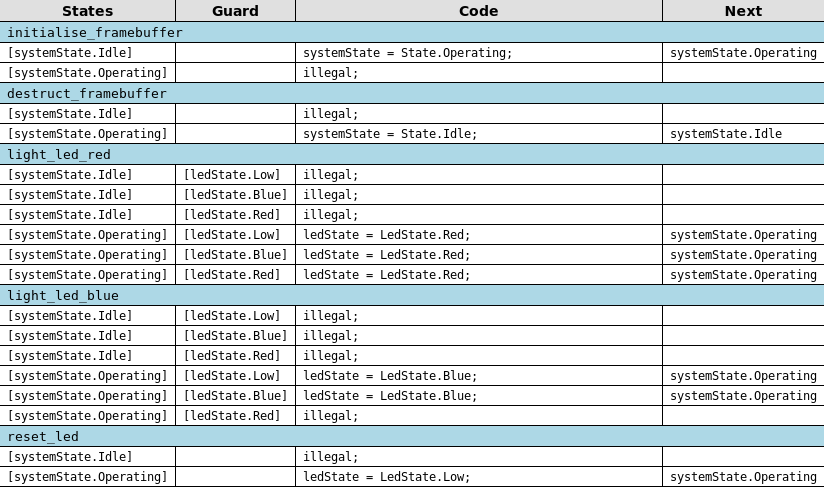
\includegraphics[width=\textwidth]{Figures/results/modelling_figures/ILEDControl/ILEDControl_event_table.png}
    \caption{The event table of \texttt{ILEDControl}}
    \label{fig:ILEDControl_event_table}
\end{figure}

We made an alternative view that shows the events per system state, as opposed to system states per event, as is the case in Figure \ref{fig:ILEDControl_event_table}. This alternative view is given in the additinoal models of Appendix \ref{Additional Models}. We have made an events per state and states per events view for all interfaces and components. The ones shown in the appendix are the ones we think convey the purpose of the interface or component the best. The alternative view can, in general, be found in Appendix \ref{Additional Models} unless the views show exactly the same, which is the case when there is just one system state and one event.
\\\\
We made a sequence diagram of a particular trace through the events of \texttt{ILEDControl}. This sequence diagram is shown in Figure \ref{fig:ILEDControl_seq}. One should note that the Dezyne behavior verifier goes through every possible sequence of events, as opposed to just one particular sequence, as is the case in the sequence diagram. The sequence diagram is useful nonetheless as a simulation of the model and to visualise certain aspects of the system. Below the sequence diagram at the bottom of Figure \ref{fig:ILEDControl_seq} we can see the next actions that can be executed at the particular state of the system. We show these possible next actions here because in the case of the \texttt{ILEDControl} interface it highlights how stating an event as \texttt{illegal} prevents one from executing the event in a trace of the system. For subsequent sequence diagram figures we will not show the possible actions explicitly, and we will only show the sequence diagram itself. As we can see in Figure \ref{fig:ILEDControl_seq}, the only available next actions are \texttt{destruct\_framebuffer}, \texttt{light\_led\_red} and \texttt{reset\_led}. \texttt{light\_led\_blue} cannot be executed because we declared it to be illegal to execute \texttt{light\_led\_blue} if the LED is already red. It is only after a \texttt{reset\_led} action that we can turn the LED blue again.

\begin{figure}[H]
    \centering
    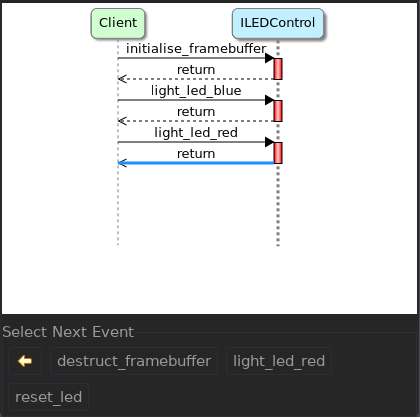
\includegraphics[width=0.5\textwidth]{Figures/results/modelling_figures/ILEDControl/ILEDControl_seq_enhanced.png}
    \caption{Sequence diagram showing a particular trace through \texttt{ILEDControl} and the next possible actions}
    \label{fig:ILEDControl_seq}
\end{figure}

\subsection{ISafetyCheck}
The next interface we will look at is \texttt{ISafetyCheck}. \texttt{ISafetyCheck} is a simple interface that specifies the behavior of the five check components, namely \texttt{KineticEnergyCheck}, \texttt{RotationalEnergyCheck}, \texttt{ArmForceCheck}, \texttt{ArmTorqueCheck} and \texttt{ArmPositionCheck}. These five safety check components implement the \texttt{ISafetyCheck} interface. We will look at these components later in this section. The single event of the \texttt{ISafetyCheck} interface is shown in Figure \ref{fig:ISafetyCheck_state_table}. In the blue row we see the \texttt{<state>.<Initial>} state. This denotes, as the name suggests, the initial state of the interface. This state is shown if an interface or component does not define any states of its own. In the case of \texttt{ISafetyCheck}, the interface is simple and need not keep track of any states of its own. The only event that the \texttt{ISafetyCheck} interface can execute is the \texttt{do\_check} event. This event denotes the execution of a safety check. Since this is an interface, \texttt{do\_check} is just a generic notion of a safety check. When we look at the components that implement \texttt{ISafetyCheck} we will see that the component associates a specific action with \texttt{do\_check}. In the Code column we can see that \texttt{do\_check} replies either the \texttt{Behavior.Safe} or \texttt{Behavior.Unsafe} behavior type. The behavior types \texttt{Behavior.Safe} and \texttt{Behavior.Unsafe} are just like boolean types, but with more indicative names.

\begin{figure}[H]
    \centering
    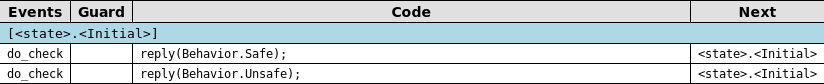
\includegraphics[width=\textwidth]{Figures/results/modelling_figures/ISafetyCheck/ISafetyCheck_state_table.png}
    \caption{State table of \texttt{ISafetyCheck}}
    \label{fig:ISafetyCheck_state_table}
\end{figure}

Figure \ref{fig:Sequence diagram of ISafetyCheck.} shows the sequence diagram we created for the \texttt{ISafetyCheck} interface. Here we make a trace through the interface, and, because this is a simulation of the model, we are free to return either \texttt{Behavior\_Safe} or \texttt{Behavior\_Unsafe} after the execution of \texttt{do\_check}.

\begin{figure}[H]
    \centering
    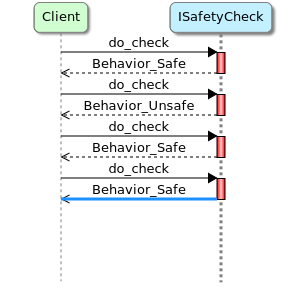
\includegraphics[width=0.5\textwidth]{Figures/results/modelling_figures/ISafetyCheck/ISafetyCheck_seq.png}
    \caption{Sequence diagram of ISafetyCheck}
    \label{fig:Sequence diagram of ISafetyCheck.}
\end{figure}

\subsection{ISensors}
% ref: section on implementation
\texttt{ISensors} defines five interfaces that correspond to a sensor or measuring device used in a safety check. The check on kinetic energy makes use of the accelerometer of the Sense HAT, the check on rotational energy makes use of the fused accelerometer, gyroscope and magnetometer data of the Sense HAT which are then used to obtain angular displacement, the arm force, torque and position are to be retrieved from robot Rose. Each \texttt{Sensor} defines only one event; this event retrieves the quantity that is to be checked. The sensors do not define any system states. In Figure \ref{fig:retrieve events} the \texttt{retrieve} events of respectively \texttt{KineticEnergyCheck}, \texttt{RotationalEnergyCheck}, \texttt{ArmForceCheck}, \texttt{ArmTorqueCheck} and \texttt{ArmPositionCheck} are given. In Figure \ref{fig:isensor_seq} their sequence diagrams are given in the same order. One may notice that the code columns define no code for these interfaces. That is because the retrieval of data is a purely implementation dependent task, and there is no control logic to check for Dezyne. In Section \ref{Binding Dezyne events to functions} it was shown how the retrieve events are bound to functions and how they are implemented.

\begin{figure}[H]
    \centering
    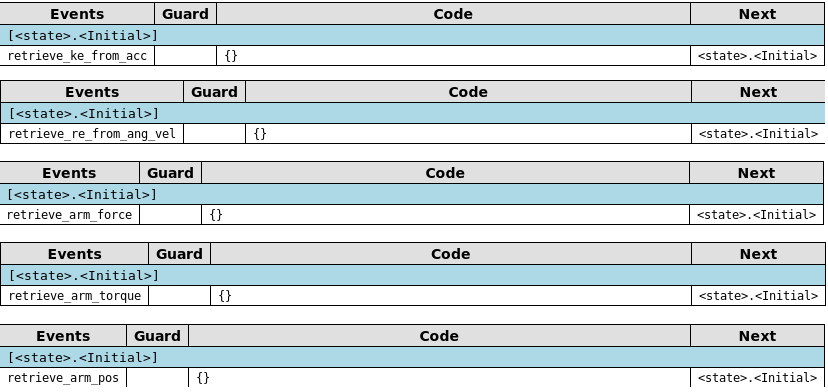
\includegraphics[width=\textwidth]{Figures/results/modelling_figures/ISensor/ISensor_state_table.png}
    \caption{State table showing the \texttt{retrieve} events of the five safety checks}
    \label{fig:retrieve events}
\end{figure}

\begin{figure}[H]
    \centering
    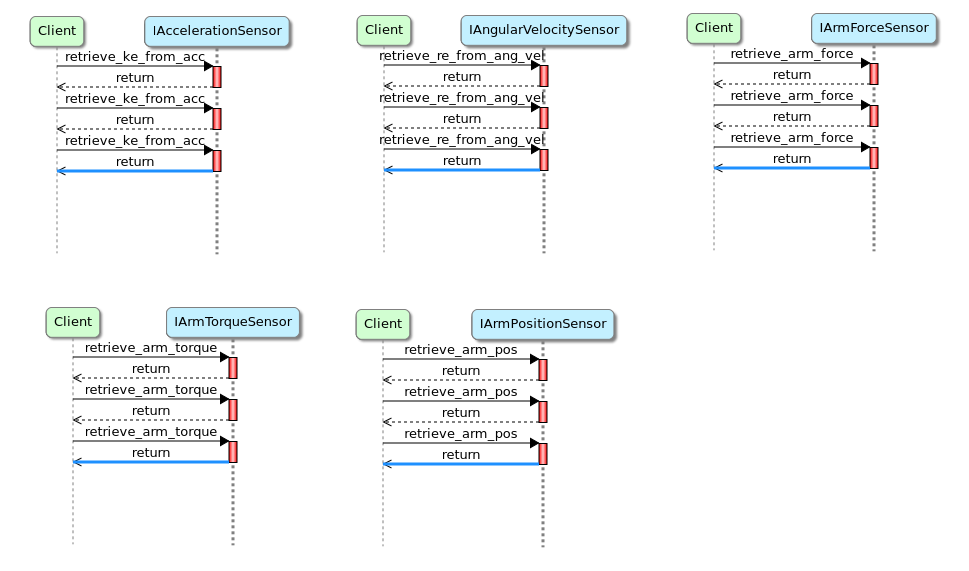
\includegraphics[width=\textwidth]{Figures/results/modelling_figures/ISensor/ISensor_seq.png}
    \caption{Sequence diagrams of the \texttt{ISensor} interfaces}
    \label{fig:isensor_seq}
\end{figure}

\subsection{IResolver}
\texttt{IResolver} is a single interface with five events that resolve values retrieved from sensors. Resolving a value in this context means translating a retrieved sensor value into something the Dezyne language can use in its control logic. Concretely, this means that the resolve events convert an obtained sensor value into \texttt{Behavior.Safe} and \texttt{Behavior.Unsafe} behavior types. This can be seen in the state table of Figure \ref{fig:IResolver_state_table}. Every resolve event either returns \texttt{Behavior.Safe} or \texttt{Behavior.Unsafe}. Later we will see that the \texttt{Controller} uses this to turn the LED blue in case of a \texttt{Behavior.Safe} reply from the resolve event and to turn the LED red in case of a \texttt{Behavior.Unsafe} reply from the resolve event. The safety check components execute their own respective resolve event. \texttt{KineticEnergyCheck} executes \texttt{resolve\_ke\_from\_acc}, \texttt{RotationalEnergyCheck} executes \texttt{resolve\_re\_from\_ang\_vel}, \texttt{ArmForceCheck} executes \texttt{resolve\_arm\_force},\\\texttt{ArmTorqueCheck} executes \texttt{resolve\_arm\_torque} and \texttt{ArmPositionCheck} executes\\\texttt{resolve\_arm\_position}.
\par
Just like with \texttt{ISafetyCheck} we are free to reply either \texttt{Behavior.Safe} or\\ \texttt{Behavior.Unsafe} in a simulation of the model, as can be seen in the sequence diagram of Figure \ref{fig:IResolver_seq}.

\begin{figure}[H]
    \centering
    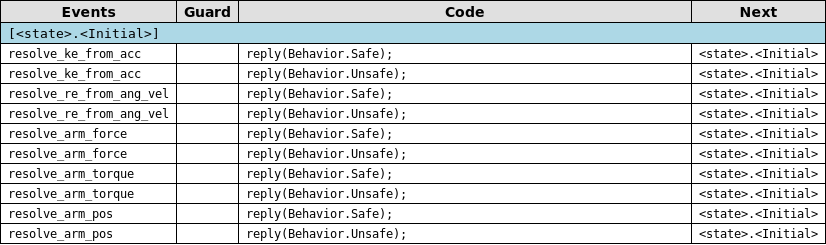
\includegraphics[width=\textwidth]{Figures/results/modelling_figures/IResolver/IResolver_state_table.png}
    \caption{State table of \texttt{IResolver}}
    \label{fig:IResolver_state_table}
\end{figure}

\begin{figure}[H]
    \centering
    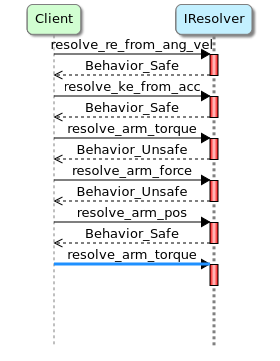
\includegraphics[width=0.45\textwidth]{Figures/results/modelling_figures/IResolver/IResolver_seq.png}
    \caption{Sequence diagram of \texttt{IResolver}}
    \label{fig:IResolver_seq}
\end{figure}

% Ref to section SQ4
One might wonder why \texttt{ISensor} consists of five separate interfaces, while \texttt{IResolver} has all resolve events in just one interface. This has to do with a useful modelling feature we used for \texttt{IResolver}. Since every safety check has to convert its retrieved sensor value to a Dezyne control logic type, and since every \texttt{resolve} action does roughly the same thing, we generalized it to one interface that is used by all checks. If we refer back to the system view of Figure \ref{fig:safety_module_system_view}, we can see this usage of \texttt{IResolver}. All checks, except \texttt{BaseCaseCheck} (\texttt{BaseCaseCheck} does not actually check anything and serves as the base case or default element for the linked list of checks), are connected to the grey square on the right edge, this is the port of \texttt{IResolver}. This port is to be bound in implementation code to functions that actually resolve or convert retrieved sensor values into Dezyne control logic.

\subsection{BaseCaseCheck}
As was mentioned in the previous section, \texttt{BaseCaseCheck} does not check any behavior of the care robot and serves as the base case or default element for the linked list of checks above it. It should always be the last element. If one wishes to add a new safety check to the system, it can be added anywhere in the list of checks, so long as it is above \texttt{BaseCaseCheck}. \texttt{BaseCaseCheck} implements the \texttt{ISafetyCheck} interface. \texttt{BaseCaseCheck} does one thing, and it does it well; in conformance with its interface, it executes the \texttt{do\_check} event. The \texttt{do\_check} event of \texttt{BaseCaseCheck} always returns \texttt{Behavior.Safe}, this is the so called base case. This is because every time we execute a check the result of this check and the directly following check will be evaluated. If one or both of the checks replies \texttt{Behavior.Unsafe}, then this \texttt{Behavior.Unsafe} value is replied further down to the controller. One might ask why one check needs to evaluate the result of the next check. This is a consequence of the linked list structure of the checks. To be clear, the controller just tasks the first check to execute. That check then executes the next check, and the next check the following check, and so towards the base case check. So it is really a particular check that executes the next check and evaluates both itself and that next check, the controller does not do this evaluation the controller. The controller only tasks the first check to execute. The task of the controller will be elaborated later this section. 
\\
Figure \ref{fig:basecasechekc_state_table} shows the state table we created for \texttt{BaseCaseCheck}. Here we see that it has only one event and always returns \texttt{Behavior.Safe}. Because the behavior of BaseCaseCheck is trivial we have omitted it here. It can be found in Section \ref{BaseCaseCheck_app} of Appendix \ref{Additional Models}.

\begin{figure}[H]
    \centering
    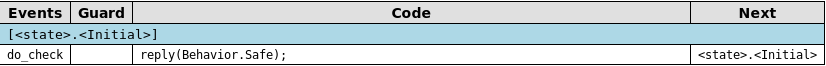
\includegraphics[width=\textwidth]{Figures/results/modelling_figures/BaseCaseCheck/BaseCaseCheck_state_table.png}
    \caption{State table of \texttt{BaseCaseCheck}}
    \label{fig:basecasechekc_state_table}
\end{figure}

\subsection{KineticEnergyCheck}
We will now look at the \texttt{KineticEnergyCheck} component. \texttt{KineticEnergyCheck} implements the \texttt{ISafetyCheck} interface and it uses the \texttt{IResolver} and \texttt{ISensors} interfaces. The state table of \texttt{KineticEnergyCheck} is shown in Figure \ref{fig:KineticEnergyCheck_state_table}. Elaborating \texttt{KineticEnergyCheck} will be straightforward, as we have already elaborated all pieces it is composed of. In Figure \ref{fig:KineticEnergyCheck_state_table} we can see that \texttt{KineticEnergyCheck} defines a single event, \texttt{do\_check}, in conformance with the interface it implements. Let us look at the Code column. Here we see that it calls the \texttt{retrieve\_ke\_from\_acc} event from the acceleration sensor interface to let the acceleration sensor obtain sensor data from the accelerometer, which can then be used to calculate kinetic energy. The raw value of kinetic energy is not usable in the Dezyne modelling language, so we convert this value to Dezyne usable control logic by calling the resolver's \texttt{resolve\_ke\_from\_acc} event. This event returns a Dezyne usable control logic type, namely \texttt{Behavior.Safe} or \texttt{Behavior.Unsafe}, which we store as the result of the \texttt{KineticEnergyCheck}. We then refer to our pointer, \texttt{iNext} which points to the next check in the list, and call the this next check. Looking back at the system view of Figure \ref{fig:safety_module_system_view}, we can see that the next check is \texttt{RotationalEnergyCheck}, but it might as well be any other check that we may add it the future. After calling the next check, we execute the \texttt{and\_safety\_states}  function, which performs a boolean AND \footnote{This is a boolean AND if we define \texttt{Behavior.Unsafe} to be $0$ and \texttt{Behavior.Safe} to be $1$. A boolean AND will only return $1$ if both proponents are $1$. In terms of our function, the \texttt{and\_safety\_states} function will only return \texttt{Behavior.Safe} if both proponents have value \texttt{Behavior.Safe}.} on the Behavior types of \texttt{KineticEnergyCheck} and the next check. The purpose of this function has to do with what we mentioned when we elaborated \texttt{BaseCaseCheck}. There we mentioned that if one or both of the checks results in behavior type \texttt{Behavior.Unsafe}, then the \texttt{and\_safety\_states} returns \texttt{Behavior.Unsafe}. Otherwise, it returns \texttt{Behavior.Safe}, which would indicate that both individual checks replied \texttt{Behavior.Safe}. Finally, since the Controller is the component that calls \texttt{KineticEnergyCheck}, the return value of the \texttt{and\_safety\_states} function is returned to the controller. The controller will decide what to do with his value.

\begin{figure}[H]
    \centering
    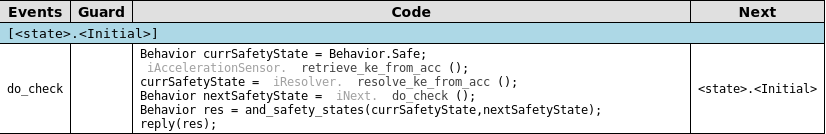
\includegraphics[width=\textwidth]{Figures/results/modelling_figures/KineticEnergyCheck/KineticEnergyCheck_state_table.png}
    \caption{State table of \texttt{KineticEnergyCheck}}
    \label{fig:KineticEnergyCheck_state_table}
\end{figure}

\texttt{KineticEnergyCheck} is a good opportunity for us to show the Dezyne verification results. The verification results are shown in Figure \ref{fig:kineticenergycheck_verification}. Verification goes from top to bottom. This indicates that, to verify \texttt{KineticEnergyCheck}, the \texttt{IAccelerationSensor}, \texttt{ISafetyCheck} and \texttt{IResolver} have to be verified first. It is only if these interfaces contain no errors that \texttt{KineticEnergyCheck} can possibly be given a positive result. It is thus convenient to model the system in such a way that is divided into chunks that can be individually verified.

\begin{figure}[H]
    \centering
    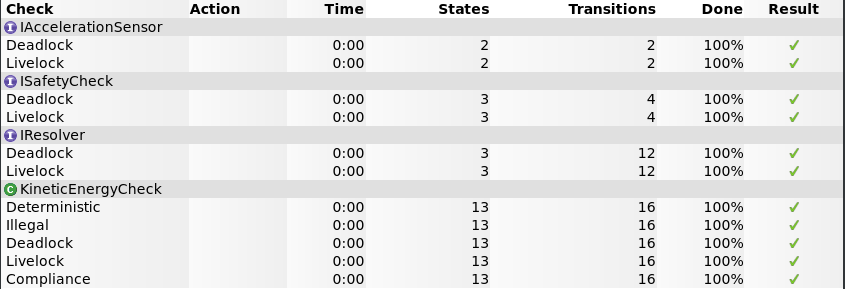
\includegraphics[width=\textwidth]{Figures/results/modelling_figures/KineticEnergyCheck/KineticEnergyCheck_verification.png}
    \caption{Verification results for the \texttt{KineticEnergyCheck} component}
    \label{fig:kineticenergycheck_verification}
\end{figure}

Let us now look at the sequence diagram of we created for \texttt{KineticEnergyCheck}. This sequence diagram is shown in Figure \ref{fig:kineticenergycheck_seq}. This sequence diagram visualises what we tried to explain concerning the \texttt{and\_safety\_states} function. \texttt{iKineticEnergyCheck} executes a \texttt{do\_check} event, which, after calling \texttt{resolve\_ke\_from\_acc}, returns either \texttt{Behavior.Safe} or \texttt{Behavior.Unsafe}. Then the \texttt{do\_check} event of the next check is executed. This next \texttt{do\_check} also returns either \texttt{Behavior.Safe} or \texttt{Behavior.Unsafe} (internally, the next check's \texttt{do\_check} event also executes a resolve action. The result of this resolve is what is actually returned by the next \texttt{do\_check}, but this is not shown). The first part of the sequence diagram of Figure \ref{fig:kineticenergycheck_seq}, starting at \texttt{iKineticEnergyCheck} all the way to \texttt{iResolver} and back to \texttt{iKineticEnergyCheck}, returns \texttt{Behavior.Safe}, because the two executed checks both returned \texttt{Behavior.Safe}. The second time we make this round, the first check returns \texttt{Behavior.Safe} and the second check returns \texttt{Behavior.Unsafe}. This results in \texttt{Behavior.Unsafe} being returned to\\\texttt{iKineticEnergyCheck}, because there was a check that returned unsafe behavior. The same holds for the third round. The fourth round returns \texttt{Behavior.Safe} again, because the two checks both returned \texttt{Behavior.Safe}. Although this is not shown in the sequence diagram, if both checks return \texttt{Behavior.Unsafe}, \texttt{Behavior.Unsafe} is returned to \texttt{iKineticEnergyCheck} as well.

\begin{figure}[H]
    \centering
    \includegraphics[width=\textwidth]{Figures/results/modelling_figures/KineticEnergyCheck/KineticEnergyCheck_seq.png}
    \caption{Sequence diagram of \texttt{KineticEnergyCheck}}
    \label{fig:kineticenergycheck_seq}
\end{figure}

\subsection{RotationalEnergyCheck, ArmForceCheck, ArmTorqueCheck and ArmPositionCheck}
\texttt{RotationalEnergyCheck},\texttt{ArmForceCheck}, \texttt{ArmTorqueCheck} and \texttt{ArmPositionCheck} all behave very similarly to \texttt{KineticEnergyCheck}, except that they call the retrieve event and resolve event for their respective quantities that they want to check. Figure \ref{fig:RotationalEnergyCheck_state_table}, Figure \ref{fig:ArmForceCheck_state_table}, Figure \ref{fig:ArmTorqueCheck_state_table} and Figure \ref{fig:ArmPositionCheck_state_table} for \texttt{RotationalEnergyCheck}, \\\texttt{ArmForceCheck}, \texttt{ArmTorqueCheck} and \texttt{ArmPositionCheck} respectively. We have omitted the sequence diagrams for these checks here. The sequence diagrams for these checks can be found in Section \ref{aRotationalEnergyCheck}, Section \ref{aArmForceCheck}, Section \ref{aArmTorqueCheck} and Section \ref{aArmPositionCheck} of Appendix \ref{Additional Models} respectively.


\begin{figure}[H]
    \centering
    \includegraphics[width=\textwidth]{Figures/results/modelling_figures/RotationalEnergyCheck/RotationalEnergyCheck_state_table.png}
    \caption{State table for \texttt{RotationalEnergyCheck}}
    \label{fig:RotationalEnergyCheck_state_table}
\end{figure}

\begin{figure}[H]
    \centering
    \includegraphics[width=\textwidth]{Figures/results/modelling_figures/ArmForceCheck/ArmForceCheck_state_table.png}
    \caption{State table for \texttt{ArmForceCheck}}
    \label{fig:ArmForceCheck_state_table}
\end{figure}

\begin{figure}[H]
    \centering
    \includegraphics[width=\textwidth]{Figures/results/modelling_figures/ArmTorqueCheck/ArmTorqueCheck_state_table.png}
    \caption{State table for \texttt{ArmTorqueCheck}}
    \label{fig:ArmTorqueCheck_state_table}
\end{figure}

\begin{figure}[H]
    \centering
    \includegraphics[width=\textwidth]{Figures/results/modelling_figures/ArmPositionCheck/ArmPositionCheck_state_table.png}
    \caption{State table for \texttt{ArmPositionCheck}}
    \label{fig:ArmPositionCheck_state_table}
\end{figure}

If one wants to add a new check to the system, this is likely going to be its base control structure also. The differences will be in the functions the retrieve and resolve functions are bound to.

\subsection{Functional behavior}
So far, when we verified the models, we have only looked at static behavior verification. At the time of writing, a prototype version of Dezyne provides us with funcional behavior verification as well. Functional behavior checking concerns itself with checks whether a system, after executing a set of actions, is in the system state that we expect it to be. We made several of these functional behavior checks. Because this is prototype functionality of the toolset, we cannot create a diagram to show the specification of such functional behavior, so we show the specification of the functional behavior in the modelling language itself.
\par
Code 5 shows the functional behavior specification for \texttt{KineticEnergyCheck}. Code 6 shows part of a modified version of \texttt{KineticEnergyCheck} that conforms with the syntax required to use the functional requirement verifier. Actually, the part that is shown is a modification of \texttt{IResolver} in which \texttt{IResolver} now part of the safety check itself and no longer returns a value, but calls either \texttt{iKineticEnergyCheck.BehaviorSafe()} or \texttt{iKineticEnergyCheck.BehaviorUnsafe()}, which corresponds to the same behavior as returning \texttt{Behavior.Safe} and \texttt{Behavior.Unsafe} respectively. In Code 5, the \texttt{Requirement} keyword is used to define a functional behavior specification. We gave this specification the name \texttt{AnyUnsafe}. This specification specifically checks if the \texttt{myState} variable has the value we expect it to be. If, in Code 6, we were to remove Line 14, this would get through the static behavior verifier as if nothing happened, but if we run this through the functional behavior verifier, we get an error, because the state does not accord with what we specified in the functional specification.


Similar functional specifications have been made for the other safety check components. For the generated source code that is to be bound to implementation code, we have used the non-functional requirement model, however, as this model has a more convenient syntax to work with.

% TODO: Why is this listing broken?
\begin{listing}
\begin{minted}[mathescape,
               numbersep=5pt,
               frame=lines,
               framesep=5mm,
               linenos]{haskell}
requirement AnyUnsafe {
	on KineticEnergyCheck;
	provides ISafetyCheck iKineticEnergyCheck;
	requires IAccelerationSensor iAccelerationSensor;
	requires ISafetyCheck iNext;
	requires IResolver iResolver;

    behaviour {
        Behavior myState = Behavior.Safe;
        bool expected = false;

        on iKineticEnergyCheck.do_check(): {
            myState = Behavior.Safe;
            expected = true;
        }

        on iNext.BehaviorUnsafe(),
            iResolver.BehaviorUnsafe(): {
            myState = Behavior.Unsafe;
            if(expected) {
                expected = false;
            } else {
                iKineticEnergyCheck.BehaviorUnsafe();
            }
        }

        on iNext.BehaviorSafe(),
            iResolver.BehaviorSafe(): {
            if(expected) {
                myState = Behavior.Safe;
                expected = false;
            } else {
                if(myState == Behavior.Safe) {
                    iKineticEnergyCheck.BehaviorSafe();
                } else {
                    iKineticEnergyCheck.BehaviorUnsafe();
                }
            }
        }
    }
}
\end{minted} 
\label{mfunctional_requirement}
\caption{Definition of \texttt{AnyUnsafe} requirement}
\end{listing}

\begin{listing}
\begin{minted}[mathescape,
               numbersep=5pt,
               frame=lines,
               framesep=5mm,
               linenos]{haskell}
on iResolver.BehaviorUnsafe(),
	iNext.BehaviorUnsafe(): {
	myState = Behavior.Unsafe;

	if(expected) {
	    expected = false;
	} else {
    	iKineticEnergyCheck.BehaviorUnsafe();
	}
}

\end{minted}

\label{modified_ke}
\caption{Edited \texttt{iResolver} for  functional verification}
\end{listing}


%%% CHAPTER
\chapter{Additional Models}
\label{Additional Models}
This Appendix provides additional models as mentioned in Section \ref{Modelling and Dezyne} of the Results.

\begin{figure}[H]
    \centering
    \includegraphics[width=0.37\textwidth]{Figures/results/modelling_figures/system_view/system_view_alt.png}
    \caption{Alternative representation of the system view given in Section \ref{System overview}.}
    \label{fig:system_view_alt}
\end{figure}


\section{ILEDControl}
\begin{figure}[H]
    \centering
    \includegraphics[width=\textwidth]{Figures/results/modelling_figures/ILEDControl/ILEDControl_state_table.png}
    \caption{State table of \texttt{ILEDControl}}
    \label{fig:ILEDControl_state_table}
\end{figure}

\begin{figure}[H]
    \centering
    \includegraphics[width=\textwidth]{Figures/results/modelling_figures/ILEDControl/ILEDControlStateChart.png}
    \caption{State chart of \texttt{ILEDControl}}
    \label{fig:ILEDControl_state_chart}
\end{figure}

\section{ISafetyCheck}

\begin{figure}[H]
    \centering
    \includegraphics[width=\textwidth]{Figures/results/modelling_figures/ISafetyCheck/ISafetyCheck_state_chart.png}
    \caption{State chart of \texttt{ISafetyCheck}}
    \label{fig:ISafetyCheck_state_chart}
\end{figure}

\section{BaseCaseCheck}
\label{BaseCaseCheck_app}

\begin{figure}[H]
    \centering
    \includegraphics[width=0.5\textwidth]{Figures/results/modelling_figures/BaseCaseCheck/BaseCaseCheck_seq.png}
    \caption{Sequence diagram of \texttt{BaseCaseCheck}}
    \label{fig:BaseCaseCheck_seq}
\end{figure}

\section{RotationalEnergyCheck}
\label{aRotationalEnergyCheck}

\begin{figure}[H]
    \centering
    \includegraphics[width=\textwidth]{Figures/results/modelling_figures/RotationalEnergyCheck/RotationalEnergyCheck_seq.png}
    \caption{Sequence diagram of \texttt{RotationalEnergyCheck}}
    \label{fig:RotationalEnergyCheck_seq}
\end{figure}


\section{ArmForceCheck}
\label{aArmForceCheck}

\begin{figure}[H]
    \centering
    \includegraphics[width=\textwidth]{Figures/results/modelling_figures/ArmForceCheck/ArmForceCheck_seq.png}
    \caption{Sequence diagram of \texttt{ArmForceCheck}}
    \label{fig:ArmForceCheck_seq}
\end{figure}


\section{ArmTorqueCheck}
\label{aArmTorqueCheck}

\begin{figure}[H]
    \centering
    \includegraphics[width=\textwidth]{Figures/results/modelling_figures/ArmTorqueCheck/ArmTorqueCheck_seq.png}
    \caption{Sequence diagram of \texttt{ArmTorqueCheck}}
    \label{fig:ArmTorqueCheck_seq}
\end{figure}



\section{RotationalEnergyCheck}
\label{aRotationalEnergyCheck}

\begin{figure}[H]
    \centering
    \includegraphics[width=\textwidth]{Figures/results/modelling_figures/ArmTorqueCheck/ArmTorqueCheck_seq.png}
    \caption{Sequence diagram of \texttt{ArmTorqueCheck}}
    \label{fig:ArmTorqueCheck_seq}
\end{figure}



\section{ArmPositionCheck}
\label{aArmPositionCheck}

\begin{figure}[H]
    \centering
    \includegraphics[width=\textwidth]{Figures/results/modelling_figures/ArmPositionCheck/ArmPositionCheck_seq.png}
    \caption{Sequence diagram of \texttt{ArmPositionCheck}}
    \label{fig:ArmPositionCheck_seq}
\end{figure}

\section{IController}
\label{IController}

\begin{figure}[H]
    \centering
    \includegraphics[width=\textwidth]{Figures/results/modelling_figures/IController/IController_event_table.png}
    \caption{Event table of \texttt{IController}}
    \label{fig:IController_event_table}
\end{figure}

\begin{figure}[H]
    \centering
    \includegraphics[width=\textwidth]{Figures/results/modelling_figures/IController/IController_state_table.png}
    \caption{State table of \texttt{IController}}
    \label{fig:IController_state_table}
\end{figure}

\begin{figure}[H]
    \centering
    \includegraphics[width=0.5\textwidth]{Figures/results/modelling_figures/IController/IController_seq.png}
    \caption{Sequence diagram of \texttt{IController}}
    \label{fig:IController_seq}
\end{figure}

\section{Controller}
\label{aController}

\begin{figure}[H]
    \centering
    \includegraphics[width=\textwidth]{Figures/results/modelling_figures/Controller/Controller_state_table.png}
    \caption{State table of \texttt{Controller}}
    \label{fig:controll_state_table}
\end{figure}


\begin{figure}[H]
    \centering
    \includegraphics[width=0.8\textwidth]{Figures/results/modelling_figures/Controller/Controller_state_chart.png}
    \caption{State chart of \texttt{Controller}}
    \label{fig:controll_old}
\end{figure}


\begin{figure}[H]
    \centering
    \includegraphics[width=\textwidth]{Figures/results/modelling_figures/Controller/old_Controller_seq.png}
    \caption{Old sequence diagram of \texttt{Controller} showing multiple checks being executed in sequence}
    \label{fig:controll_old}
\end{figure}



\chapter{Source code}
\label{Source code}
We have included important code snippets here that are relevant to Section \ref{Implementation} of the Results. The code listed here may be outdated. The code on \href{https://github.com/Yousousen/safety-module-for-care-robot-rose}{the repository} is guaranteed to be up-to-date.

\section{Main and roll functions}
\label{main and roll}
This section contains the \texttt{main} and \texttt{roll} functions. \texttt{main} calls \texttt{roll} immediately after initialation of the safety module. The \texttt{roll} function does more initialization, like binding the Dezyne resolve, retrieve and light\_led events and starting the threads. The main thread runs indefinitely, waiting for input to acknowledge unsafe behavior and reset the LED matrix. Created threads run besides the main thread to continuously retrieve and sample sensor data.
\begin{minted}[mathescape,
               numbersep=5pt,
               frame=lines,
               framesep=5mm,
               linenos]{c++}
               
auto main() -> int {
    initialise();
    int r = roll();
    if (r != OK) return EXIT_FAILURE;
    destruct();
}

}
ErrorCode_t roll() {
    // Initialise dezyne locator and runtime.
    IResolver iResolver({});

    // Bind resolvers
    iResolver.in.resolve_ke_from_acc = []() -> Behavior::type {
        int r;
        Behavior::type type;
        double ke;

        r = safe_call([&ke]() { ke = kinetic_energy; }, &mutex["ke"]);
        if (r != OK) exit(EXIT_FAILURE);

        if (ke > MAX_KE)
            type = Behavior::type::Unsafe;
        else
            type = Behavior::type::Safe;
        return type;
    };

    iResolver.in.resolve_re_from_ang_vel = []() -> Behavior::type {
        int r;
        Behavior::type type;
        double re;

        r = safe_call([&re]() { re = rotational_energy; }, &mutex["re"]);
        if (r != OK) exit(EXIT_FAILURE);

        if (re > MAX_RE)
            type =  Behavior::type::Unsafe;
        else
            type =  Behavior::type::Safe;
        return type;
    };

    iResolver.in.resolve_arm_force = []() -> Behavior::type {
        int r;
        Behavior::type type;
        double str;
        bool has_payload;

        r = safe_call([&]() { str = arm_force; has_payload =
                arm_has_payload(); }, &mutex["arm_force"]);
        if (r != OK) exit(EXIT_FAILURE);

        if ( has_payload && str > MAX_FORCE_PAYLOAD)
            type = Behavior::type::Unsafe;
        else if (str > MAX_FORCE)
            type = Behavior::type::Unsafe;
        else
            type = Behavior::type::Safe;
        return type;
    };

    iResolver.in.resolve_arm_torque = []() -> Behavior::type {
        int r;
        Behavior::type type;
        double str;
        bool has_payload;

        r = safe_call([&]() { str = arm_torque; has_payload =
                arm_has_payload(); }, &mutex["arm_torque"]);
        if (r != OK) exit(EXIT_FAILURE);

        if ( has_payload && str > MAX_TORQUE_PAYLOAD)
            type = Behavior::type::Unsafe;
        else if (str > MAX_torque)
            type = Behavior::type::Unsafe;
        else
            type = Behavior::type::Safe;
        return type;
    };

    iResolver.in.resolve_arm_pos = []() -> Behavior::type {
        int r;
        Behavior::type type;
        bool folded;
        bool is_moving;

        r = safe_call([&]() { folded = arm_is_folded(); is_moving =
                robot_is_moving(); }, &mutex["arm_pos"]);
        if (r != OK) exit(EXIT_FAILURE);

        if (is_moving && !folded)
            type = Behavior::type::Unsafe;
        else
            type = Behavior::type::Safe;
        return type;
    };

    dzn::locator locator;
    dzn::runtime runtime;
    locator.set(runtime);
    locator.set(iResolver);
    auto output = std::ofstream("dzn_output.log");
    locator.set(static_cast<std::ostream&>(output));

    System s(locator);
    s.dzn_meta.name = "System";

    /*
     * Bind dezyne functions with C++ functions.
     */
    /* s.iController.out.what_triggered = what_triggered; */
    s.iLEDControl.in.initialise_framebuffer = initialise_framebuffer;
    s.iLEDControl.in.destruct_framebuffer = destruct_framebuffer;
    s.iLEDControl.in.light_led_red = dzn_light_led;
    s.iLEDControl.in.light_led_blue = dzn_light_led;
    s.iLEDControl.in.reset_led = reset_led;
    s.iController.out.initialise_imu = initialise_imu;
    s.iController.out.initialise_mutexes = initialise_mutexes;
    s.iController.out.initialise_semaphores = initialise_semaphores;
    s.iController.out.destruct_mutexes = destruct_mutexes;
    s.iController.out.destruct_semaphores = destruct_semaphores;
    s.iAccelerationSensor.in.retrieve_ke_from_acc = dzn_retrieve_ke_from_acc;
    s.iAngularVelocitySensor.in.retrieve_re_from_ang_vel =
        dzn_retrieve_re_from_ang_vel;
    s.iArmPositionSensor.in.retrieve_arm_pos = dzn_retrieve_arm_pos;
    s.iArmForceSensor.in.retrieve_arm_force = dzn_retrieve_arm_force;
    s.iArmTorqueSensor.in.retrieve_arm_torque = dzn_retrieve_arm_torque;


    // Check bindings
    s.check_bindings();

    /*
     * Initialise system
     */
    s.iController.in.initialise();

    /*** Threads related ***/
    struct sched_param rtparam = { .sched_priority = 42 };
    pthread_attr_t rtattr, nrtattr;
    sigset_t set;
    int sig;

    // real-time thread that starts safety checks periodically.
    static pthread_t th_rt_checks;
    // real-time thread for lighting the LED matrix.
    static pthread_t th_rt_light_led;
    // real-time threads for retrieving data.
    static pthread_t th_rt_ret_acc, th_rt_ret_ang_disp;
    static pthread_t th_rt_ret_arm_force, th_rt_ret_arm_torque, th_rt_ret_arm_pos;
    // real-time threads for sampling sensor data.
    static pthread_t th_rt_sample_acc, th_rt_sample_ang_disp;

    // non-real-time thread for lighting the LED matrix.
    static pthread_t th_nrt_light_led;
    // non-real-time thread for retrieving sensor data from the IMU and ROS.
    static pthread_t th_nrt_ret_imu, th_nrt_ret_arm_force;
    static pthread_t th_nrt_ret_arm_torque, th_nrt_ret_arm_pos;

    // Information about periodic  threads.
    static struct th_info th_info;

    // Arguments to threads.
    struct threadargs threadargs;

    sigemptyset(&set);
    sigaddset(&set, SIGINT);
    sigaddset(&set, SIGTERM);
    sigaddset(&set, SIGHUP);

    pthread_attr_init(&nrtattr);
    pthread_attr_setdetachstate(&nrtattr, PTHREAD_CREATE_JOINABLE);
    pthread_attr_setinheritsched(&nrtattr, PTHREAD_EXPLICIT_SCHED);
    pthread_attr_setschedpolicy(&nrtattr, SCHED_OTHER);

    pthread_attr_init(&rtattr);
    pthread_attr_setdetachstate(&rtattr, PTHREAD_CREATE_JOINABLE);
    pthread_attr_setinheritsched(&rtattr, PTHREAD_EXPLICIT_SCHED);
    pthread_attr_setschedpolicy(&rtattr, SCHED_FIFO);
    pthread_attr_setschedparam(&rtattr, &rtparam);

    /*** Start threads ***/
    // Start thread rt_light_led
    errno = pthread_create(&th_rt_light_led, &rtattr, &rt_light_led, NULL);
    if (errno)
        fail("pthread_create");

    // Start thread rt_retrieve_acceleration
    errno = pthread_create(&th_rt_ret_acc, &rtattr, &rt_retrieve_acceleration,
            &threadargs);
    if (errno)
        fail("pthread_create");

    // Start thread rt_retrieve_angular_displacement
    errno = pthread_create(&th_rt_ret_ang_disp, &rtattr,
            &rt_retrieve_angular_displacement, &threadargs);
    if (errno)
        fail("pthread_create");

    // Start thread rt_retrieve_arm_force
    errno = pthread_create(&th_rt_ret_arm_force, &rtattr,
            &rt_retrieve_arm_force, &threadargs);
    if (errno)
        fail("pthread_create");

    // Start thread rt_retrieve_arm_torque
    errno = pthread_create(&th_rt_ret_arm_torque, &rtattr,
            &rt_retrieve_arm_torque, &threadargs);
    if (errno)
        fail("pthread_create");

    // Start thread rt_retrieve_arm_position
    errno = pthread_create(&th_rt_ret_arm_pos, &rtattr,
            &rt_retrieve_arm_position, &threadargs);
    if (errno)
        fail("pthread_create");

    // Start thread rt_sample_acceleration
    errno = pthread_create(&th_rt_sample_acc, &rtattr, &rt_sample_acceleration,
            &threadargs);
    if (errno)
        fail("pthread_create");

    // Start thread rt_sample_angular_velocity
    errno = pthread_create(&th_rt_sample_ang_disp, &rtattr,
            &rt_sample_angular_velocity, &threadargs);
    if (errno)
        fail("pthread_create");

    // Start thread nrt_light_led
    errno = pthread_create(&th_nrt_light_led, &nrtattr, &nrt_light_led, (void*)
            &threadargs);
    if (errno)
        fail("pthread_create");

    // Start thread nrt_retrieve_imu
    errno = pthread_create(&th_nrt_ret_imu, &nrtattr,
            &nrt_retrieve_imu, NULL);
    if (errno)
        fail("pthread_create");

    // Start thread nrt_retrieve_arm_force
    errno = pthread_create(&th_nrt_ret_arm_force, &nrtattr,
            &nrt_retrieve_arm_force, NULL);
    if (errno)
        fail("pthread_create");

    // Start thread nrt_retrieve_arm_torque
    errno = pthread_create(&th_nrt_ret_arm_torque, &nrtattr,
            &nrt_retrieve_arm_torque, NULL);
    if (errno)
        fail("pthread_create");

    // Start thread nrt_retrieve_arm_position
    errno = pthread_create(&th_nrt_ret_arm_pos, &nrtattr,
            &nrt_retrieve_arm_position, NULL);
    if (errno)
        fail("pthread_create");



    printf("Started running indefinitely.\n");
    std::string input;
#if PERIODIC_CHECKS
    printf("press: q to quit, r to reset\n");

    th_info.body = rt_checks;
    /* th_info.period = 1E6*4;   // 4s */
    /* th_info.period = 1E6/4;      // 250ms */
    th_info.period = imu_poll_interval;      // poll interval based period.
    th_info.s = &s;
    // Start periodic real-time checks.
    errno = pthread_create(&th_rt_checks, &rtattr, &rt_periodic_thread_body,
            &th_info);
    if (errno)
        fail("pthread_create");

    // The safety module runs so long we are in this loop. The LED light can be
    // reset by inputting 'r'.  We quit the loop correctly by inputting 'q'.
    while (1) {
        std::cin >> input;
        /* input = "a"; */
        if (input == "q") {
            break;
        } else if (input == "r") {
            s.iController.in.reset();
        } else if (input == "i") {
            // Purposely here to show illegal exception handler.
            s.iController.in.initialise();
        } else {
            printf("Did not understand input.\n");
        }
    }
#else
    while (1) {
        printf("press: q to quit, d to execute all checks, r to reset\n");
        printf("a to check acc, aa to check ang acc, s to check str, p to check pos\n\n> ");

        // Notify nrt_retrieve_acceleration that it can retrieve acceleration.
        /* sem_post(&semaphore["retrieve_acc"]]); */
        // Notify rt_sample_acceleration that it can go sample acceleration.
        /* sem_post(&sem_sample_acc); */

        std::cin >> input;
        /* input = "a"; */
        if (input == "q") {
            break;
        } else if (input == "d") {
            s.iController.in.do_checks();
        } else if (input == "r") {
            s.iController.in.reset();
        } else if (input == "i") {
            // Purposely here to show illegal exception handler.
            s.iController.in.initialise();
        } else {
            printf("Did not understand input.\n");
        }
    }
#endif
    printf("Stopping\n");

    // Destruct system
    s.iController.in.destruct();

    // Kill threads
    pthread_cancel(th_nrt_light_led);
    pthread_cancel(th_nrt_ret_arm_force);
    pthread_cancel(th_nrt_ret_arm_torque);
    pthread_cancel(th_nrt_ret_arm_pos);
    pthread_cancel(th_nrt_ret_imu);
    pthread_cancel(th_rt_light_led);
    pthread_cancel(th_rt_ret_acc);
    pthread_cancel(th_rt_ret_ang_disp);
    pthread_cancel(th_rt_ret_arm_force);
    pthread_cancel(th_rt_ret_arm_torque);
    pthread_cancel(th_rt_ret_arm_pos);
    pthread_cancel(th_rt_sample_acc);
    pthread_cancel(th_rt_sample_ang_disp);

#if PERIODIC_CHECKS
    pthread_cancel(th_rt_checks);
#endif

    pthread_join(th_nrt_light_led, NULL);
    pthread_join(th_nrt_ret_arm_pos, NULL);
    pthread_join(th_nrt_ret_arm_force, NULL);
    pthread_join(th_nrt_ret_arm_torque, NULL);
    pthread_join(th_nrt_ret_imu, NULL);
    pthread_join(th_rt_light_led, NULL);
    pthread_join(th_rt_ret_acc, NULL);
    pthread_join(th_rt_ret_ang_disp, NULL);
    pthread_join(th_rt_ret_arm_force, NULL);
    pthread_join(th_rt_ret_arm_torque, NULL);
    pthread_join(th_rt_ret_arm_pos, NULL);
    pthread_join(th_rt_sample_acc, NULL);
    pthread_join(th_rt_sample_ang_disp, NULL);

#if PERIODIC_CHECKS
    pthread_join(th_rt_checks, NULL);
#endif

    return OK;
}
\end{minted}

\section{Periodic thread functions}
This code snippet shows the rt\_checks and rt\_periodic\_thread\_body functions. These are used to periodically execute the checks. rt\_checks shows us calling the the Dezyne do\_checks() function. The thread that starts \texttt{rt\_checks} itself was shown in Section \ref{main and roll} of the Appendix.
               
\begin{minted}[mathescape,
               numbersep=5pt,
               frame=lines,
               framesep=5mm,
               linenos]{c++}

static void rt_checks(void* arg) {
    struct threadargs *args = (struct threadargs *)arg;
    /*
     * Since do_checks is implemented in Dezyne, if we want to disable one
     * check we have to remove the check from the linked list in System.dzn.
     * This is a consequence of making the system more generic. 
     */
    (args->s)->iController.in.do_checks();
}

static void *rt_periodic_thread_body(void *arg) {
    struct periodic_task *ptask;
    struct th_info* the_thread = (struct th_info*) arg;
    struct threadargs threadargs;

    // Copy over dezyne system pointer
    threadargs.s = the_thread->s;

    ptask = start_periodic_timer(0, the_thread->period);
    if (ptask == NULL) {
        printf("Start Periodic Timer");

        return NULL;
    }

    while(1) {
        wait_next_activation(ptask);
        the_thread->body((void*) &threadargs);
    }

    return NULL;
}

struct periodic_task *start_periodic_timer(unsigned long long offset_in_us,
        int period) {
    struct periodic_task *ptask;

    ptask = (struct periodic_task*) malloc(sizeof(struct periodic_task));
    if (ptask == NULL) {
        return NULL;
    }

    // Current time is added first, we let the thread wait for its next
    // activation using absolute time.
    clock_gettime(CLOCK_REALTIME, &ptask->ts);
    timespec_add_us(&ptask->ts, offset_in_us);
    ptask->period = period;
    return ptask;
}

void wait_next_activation(struct periodic_task *ptask) {
    // Suspend the thread until the time value specified by &t->ts has elapsed.
    // Note the use of absolute time.
    clock_nanosleep(CLOCK_REALTIME, TIMER_ABSTIME, &ptask->ts, NULL);
    // Add another period to the time specification.
    timespec_add_us(&ptask->ts, ptask->period);
}

\end{minted}

\section{Lighting LED functions}
This snippet shows all function called in a complete line of communication from Dezyne to the driver as was shown in Figure \ref{fig:led_threads}. \texttt{dzn\_light\_led} is executed from the main thread, \texttt{rt\_light\_led} and \texttt{nrt\_light\_led} are executed from their own threads. The \texttt{reset\_led} functions are identical in structure and differ only in that they have the task of resetting the LED matrix instead of lighting the LED matrix red or blue.

\begin{minted}[mathescape,
               numbersep=5pt,
               frame=lines,
               framesep=5mm,
               linenos]{c++}
void dzn_light_led(char* color) {
    // Set color
    int r = safe_call([=]() { strcpy(::color, color); }, &mutex["color"]);

    if (r != OK) exit(EXIT_FAILURE);
    // Let rt_light_led know that it can send a color to nrt_light_led.
    sem_post(&semaphore["led"]);
}


static void* rt_light_led(void* arg) {
    int n = 0;
    int len;
    int ret;
    int r;
    int s;
    char buf[128];
    struct sockaddr_ipc saddr;
    size_t poolsz;

    struct threadargs *args = (struct threadargs *) arg;
    // Initialise XDDP
    /*
     * Get a datagram socket to bind to the RT endpoint. Each
     * endpoint is represented by a port number within the XDDP
     * protocol namespace.
     */
    s = socket(AF_RTIPC, SOCK_DGRAM, IPCPROTO_XDDP);
    if (s < 0) {
        perror("socket");
        exit(EXIT_FAILURE);
    }

    /*
     * Set a local 16k pool for the RT endpoint. Memory needed to
     * convey datagrams will be pulled from this pool, instead of
     * Xenomai's system pool.
     */
    poolsz = 16384; /* bytes */
    ret = setsockopt(s, SOL_XDDP, XDDP_POOLSZ, &poolsz, sizeof(poolsz));
    if (ret)
        fail("setsockopt");
    /*
     * Bind the socket to the port, to setup a proxy to channel
     * traffic to/from the Linux domain.
     *
     * saddr.sipc_port specifies the port number to use.
     */
    memset(&saddr, 0, sizeof(saddr));
    saddr.sipc_family = AF_RTIPC;
    saddr.sipc_port = XDDP_PORT_LIGHT_LED;
    ret = bind(s, (struct sockaddr *)&saddr, sizeof(saddr));
    if (ret)
        fail("bind");

    /*
     * Send a datagram to the NRT endpoint via the proxy.
     * We may pass a NULL destination address, since a
     * bound socket is assigned a default destination
     * address matching the binding address (unless
     * connect(2) was issued before bind(2), in which case
     * the former would prevail).
     */
    while (1) {
        // Wait for an up to send a color to the LED matrix.
        sem_wait(&semaphore["led"]); 
        char msg[SIZE];

        // Get color
        r = safe_call([&msg]() { strcpy(msg, color); }, &mutex["color"]);
        if (r != OK) exit(EXIT_FAILURE);

        len = strlen(msg);
        ret = sendto(s, msg, len, 0, NULL, 0);
        if (ret != len)
            fail("sendto");
        /* printf("%s: sent %d bytes, \"%.*s\"\n", __FUNCTION__, ret, ret, msg); */
    }
    return NULL;
}


static void* nrt_light_led(void *arg) {
    int r;
    struct threadargs *args = (struct threadargs *)arg;

    char buf[128], *devname;
    int fd, ret;
    if (asprintf(&devname, "/dev/rtp%d", XDDP_PORT_LIGHT_LED) < 0)
        fail("asprintf");
    fd = open(devname, O_RDWR);
    free(devname);
    if (fd < 0)
        fail("open");

    while (1) {
        /* Get the next message from rt_light_led. */
        /* read what to color the led buffer in */
        ret = read(fd, buf, sizeof(buf));
        if (ret <= 0)
            fail("read");

        // Convert hex string to int.
        int color = (int)strtol(buf, NULL, 16);

        r = safe_call([=]() { light_led(color); }, &mutex["color"]);
        if (r != OK) exit(EXIT_FAILURE);
    }

    return NULL;
}



\end{minted}

\section{Retrieving angular displacement functions}
This code snippet shows all functions called in a complete line of communication from Dezyne to the driver as was shown in Figure \ref{fig:quantity_threads}. \texttt{dzn\_retrieve\_angular\_displacement} is called from the main thread, \texttt{rt\_sample\_angular\_displacement},\\\texttt{rt\_retrieve\_angular\_displacment} and \texttt{nrt\_retrieve\_imu} run in their own threads. The other function structures for retrieval of data are identical except that they retrieve (and sample) a different quanity.

\begin{minted}[mathescape,
               numbersep=5pt,
               frame=lines,
               framesep=5mm,
               linenos]{c++}
void dzn_retrieve_angular_displacement() {
    // Currently implemented in sample_angular_displacement itself.
}


static void* rt_retrieve_angular_displacement(void* arg) {
    int n = 0;
    int len;
    int ret;
    int r;
    int s;
    char buf[BUFSIZE];
    struct sockaddr_ipc saddr;
    size_t poolsz;

    struct threadargs *args = (struct threadargs *)arg;

    // Initialise XDDP
    /*
     * Get a datagram socket to bind to the RT endpoint. Each
     * endpoint is represented by a port number within the XDDP
     * protocol namespace.
     */
    s = socket(AF_RTIPC, SOCK_DGRAM, IPCPROTO_XDDP);
    if (s < 0) {
        perror("socket");
        exit(EXIT_FAILURE);
    }

    /*
     * Set a local 16k pool for the RT endpoint. Memory needed to
     * convey datagrams will be pulled from this pool, instead of
     * Xenomai's system pool.
     */
    poolsz = 16384; /* bytes */
    ret = setsockopt(s, SOL_XDDP, XDDP_POOLSZ, &poolsz, sizeof(poolsz));
    if (ret)
        fail("setsockopt");
    /*
     * Bind the socket to the port, to setup a proxy to channel
     * traffic to/from the Linux domain.
     *
     * saddr.sipc_port specifies the port number to use.
     */
    memset(&saddr, 0, sizeof(saddr));
    saddr.sipc_family = AF_RTIPC;
    saddr.sipc_port = XDDP_PORT_RET_ANG_DISP;
    ret = bind(s, (struct sockaddr *)&saddr, sizeof(saddr));
    if (ret)
        fail("bind");

    /*
     * Retrieve a datagrams from the NRT endpoint via the proxy.
     */
    while (1) {
        // Read packets echoed by the non-real-time thread.
        /*
         * This call blocks if there is no data to receive. This however is not
         * a problem as sample angular velocity is not depended on this thread
         * blocking or not. That is, sample angular velocity can do its work
         * independent of this thread.
         */
        ret = recvfrom(s, buf, sizeof(buf), 0, NULL, 0);
        if (ret <= 0)
            fail("recvfrom");
        /* printf("   => \"%.*s\" received by peer\n", ret, buf); */
        n = (n + 1) % (sizeof(buf) / sizeof(buf[0]));

        // Set angular displacement
        r = safe_call([&buf]() { set_angular_displacement(atof(buf)); },
                &mutex["ang_disp"]);
        if (r != OK) exit(EXIT_FAILURE);
    }
    return NULL;
}


static void* nrt_retrieve_imu(void *arg) {
    struct threadargs *args = (struct threadargs *)arg;

    char *devname;
    int fd_acc, fd_ang_disp, ret;

    // file descriptor for acceleration.
    if (asprintf(&devname, "/dev/rtp%d", XDDP_PORT_RET_ACC) < 0)
        fail("asprintf");
    fd_acc = open(devname, O_RDWR);
    free(devname);
    if (fd_acc < 0)
        fail("open");

    // file descriptor for angular velocity.
    if (asprintf(&devname, "/dev/rtp%d", XDDP_PORT_RET_ANG_DISP) < 0)
        fail("asprintf");
    fd_ang_disp = open(devname, O_RDWR);
    free(devname);
    if (fd_ang_disp < 0)
        fail("open");

    while (1) {
        double acc_largest, accx, accy, accz;
        double ang_disp_largest, ang_dispx, ang_dispy, ang_dispz;
        // Wait for an up before retrieving acceleration from the sense hat
        // driver.
        /* sem_wait(&semaphore["retrieve_acc"]); */

        // Poll at the rate recommended by the IMU.
        usleep(imu_poll_interval);

        while (imu->IMURead()) {
            RTIMU_DATA imuData = imu->getIMUData();
            accx = gforce_to_si(imuData.accel.x());
            accy = gforce_to_si(imuData.accel.y());
            accz = gforce_to_si(imuData.accel.z()-1); // -1 subtracts gravity.
            // angular velocity is in radians.
            ang_dispx = imuData.fusionPose.x();
            ang_dispy = imuData.fusionPose.y();
            ang_dispz = imuData.fusionPose.z();
        }

        /*
         * For both acceleration ang angular velocity, determine which axis had
         * the largest increase. The largest increase will be used to
         * respectively calculate kinetic energy and rotational energy.
         */
        accx = fabs(accx);
        accy = fabs(accy);
        accz = fabs(accz);
        ang_dispx = fabs(ang_dispx);
        ang_dispy = fabs(ang_dispy);
        ang_dispz = fabs(ang_dispz);

        if (accx > accy && accx > accz)
            acc_largest = accx;
        else if (accy > accx && accy > accz)
            acc_largest = accy;
        else
            acc_largest = accz;

        if (ang_dispx > ang_dispy && ang_dispx > ang_dispz)
            ang_disp_largest = ang_dispx;
        else if (ang_dispy > ang_dispx && ang_dispy > ang_dispz)
            ang_disp_largest = ang_dispy;
        else
            ang_disp_largest = ang_dispz;

        // Write retrieved acceleration to rt_retrieve_acceleration.
        write_to_fd(fd_acc, acc_largest);
        // Write retrieved angular velocity to rt_retrieve_angular_displacement.
        write_to_fd(fd_ang_disp, ang_disp_largest);
    }

    return NULL;
}


\end{minted}


\end{appendices}

%%%% GLOSSARY %%%

\newglossaryentry{4g}
{
        name=4G,
        description={4G is the fourth generation of broadband cellular network technology, succeeding 3G. }
}
\newglossaryentry{pi}{
    name={Raspberry Pi},
    description={The raspberry pi is a low cost high performance computer series created by the Rasberry Pi Foundation.}
}

\newglossaryentry{wifi}{
name={WiFi},
description={A local area network that uses high frequency radio signals to transmit and receive data over distances of a few hundred feet; uses ethernet protocol}
}

\newglossaryentry{mcuu}{
name={microcontroller},
description={A microcontroller (MCU for microcontroller unit) is a small computer on a single metal-oxide-semiconductor (MOS) integrated circuit chip}
}

\newglossaryentry{fpga}{
name=FPGA,
description={It is an acronym for field programmable gate array. It is a semiconductor IC where a large majority of the electrical functionality inside the device can be changed; changed by the design engineer, changed during the PCB assembly process, or even changed after the equipment has been shipped to customers out in the 'field'.}
}

\newacronym{mcu}{MCU}{microcontroller}
\newacronym{ros}{ROS}{Robot Operating System}
\newacronym{fpga}{FPGA}{Field Programmable Gate Array}


\clearpage
\printglossary
\clearpage
\printglossary[type=\acronymtype]




% Bibliography
\printbibliography
\addcontentsline{toc}{chapter}{Bibliography}
\nocite{apa_richtlijnen}


\newpage
\chapter*{Summary}
\addcontentsline{toc}{chapter}{Summary}

Research group Robotics develops a care robot, called Rose, which is able to assist elderly people with every day tasks. Although Rose has some measures of safety built into her system, robot Rose lacks the kind of guarantees on safety that are required to use Rose in practice. To improve the safety of robot Rose, research group Robotics at Inholland Alkmaar wants to create a safety module which checks the behavior of Rose and which gives a signal when Rose performs an unsafe action, where an unsafe action is characterized by an action that will cause a collision with a human or object, an action that will cause Rose to clamp with a human or object, or an action that will cause Rose her grip arm to pinch a human or an object.
\\\\
Our research focuses on laying down a basis for this safety module, from which further research can build upon. This research is a feasibility study in the sense that we want to explore existing ideas in mobile robotic safety, real-time robotic systems and verification of system behavior. The goal of this research is to apply these existing ideas to our case with robot Rose, and to provide a prototype of the safety module to affirm the feasibility of the system as a whole. In order to achieve this goal, we setup the following principal research question: \textit{\mq}. To provide an answer to this question the research was divided into four parts, these are: obtaining a hardware platform and a real-time operating system for the implementation, devising a way to use sensor data to detect unsafe actions and devising a way to signal this to the environment, creating a formal specification of the behavior of safety module, and creating an implementation using the obtained hardware platform, operating system and created formal specification.
\\\\
Firstly, we conducted a literature review and comparative study to decide on a hardware platform and real-time operating system to use. The literature review and the comparative study showed the \gls{pi} to be the best hardware platform and Raspbian Buster with the Xenomai framework to be the best real-time operating system to fulfill the goal of the research.
\par
Secondly, we reasoned that unsafe actions can be detected by checking the kinetic energy, rotational energy, grip arm force, grip arm torque and the position of the grip arm of robot Rose. The \gls{pi} has a Sense HAT with sensors that are used to obtain kinetic energy and rotational energy. The grip arm values are implemented as stubs that simulate force, torque and position values respectively. Unsafe actions are signalled by turning the LED matrix of the Sense HAT red.
\par
Thirdly, a model of the safety module was made in a formal specification language to verify and assert correct and anticipated behavior of the safety module.
\par
Lastly, the safety module was implemented, using the formal model, on the hardware platform and real-time operating system.
\\\\
Running the safety module showed anticipated behavior; excessive kinetic energy and excessive rotational energy are detected and signalled.
\\\\
From tests we concluded that the safety module achieves soft real-time operation. Furthermore, because of the successful runs of demonstrations of the safety module, we affirmed the feasibility of using this hardware and operating system setup, and we concluded that  the goal of designing and implementing a safety module that provides an extra layer of safety in order to prevent injury to patients or damage to the environment because of collision, clamping or pinching has been achieved.
\\\\
The safety module sometimes has issues with the timeliness in signalling unsafe actions. We therefore recommend follow-up research to improve the timeliness of the safety module. Moreover, we recommend follow-up research to improve the safety module by setting sight on achieving hard real-time operation.

\end{document}